\documentclass{article}

% Language setting
% Replace `english' with e.g. `spanish' to change the document language
\usepackage[spanish]{babel}

% Set page size and margins
% Replace `letterpaper' with `a4paper' for UK/EU standard size
\usepackage[letterpaper,top=2cm,bottom=2cm,left=3cm,right=3cm,marginparwidth=1.75cm]{geometry}

% Useful packages
\usepackage{graphicx}
\usepackage[colorlinks=true, allcolors=blue]{hyperref}
\usepackage{diagbox}
\usepackage{subcaption}
\usepackage{placeins}


\title{Resultados Opinión Dinámica de Opiniones bajo Estructura de Comunidades}

\begin{document}




    \section{Código}
    Para este experimento se ha tenido que generar las siguientes clases:
    \begin{itemize}
        \item \textbf{GraphFactory}: Es el encargado de crear el grafo en funcion del numero de nodos, aristas, comunidades y el probabilidad interconexion
        \item \textbf{GraphDW}: Es el encargado de coger el grafo y ejecutar el model DW sobre el. Tiene como parametro la velocidad de convergencia, umbral de confianza y valor de parada.
        \item \textbf{ExecuteMonteCarlo}: Es el encargado de ejecutar MonteCarlo con el grafo DW. Tiene como parametro el numero de ejecuciones que se va a realizar. Y de salida devuelve la media de pasos que se ha tardado para llegar a la convergencia y dibuja un grafo de cada paso.
    \end{itemize}

    Todo este código esta en mi \href{https://github.com/DaniMG95/community-opinion-dynamics}{repositorio}.

    \section{Tabla de resultados}
    Finalmente se lanzo todos los monte Carlo con una media de 30 ejecuciones y los resultados fueron los siguiente.

    \begin{table}[h]
        \centering
        \begin{tabular}{|l|c|c|c|c|c|}
            \hline
            \diagbox{Prob. inter}{umbral confianza} & 0.1 & 0.15 & 0.2 & 0.25 & 0.3 \\ \hline
            0.3 & 708666 & 314000 & 189833 & 138666 & 75000 \\ \hline
            0.5 & 723833 & AA & 203333 & 152833 & 76166 \\ \hline
            0.7 & 823833 & 399833 & 256833 & 168166 & 79666 \\ \hline
            0.9 & 1632166 & 826500 & 478166 & 337166 & 162166 \\ \hline
        \end{tabular}
        \caption{Ejemplo de tabla con división diagonal}
    \end{table}

    \section{Gráficas}

    \subsection{Prob. inter 0.3, confianza 0.1}

    \subsection{Prob. inter 0.3, confianza 0.15}
    \begin{figure}[htbp]
        \centering
        \begin{subfigure}[b]{0.32\linewidth}
            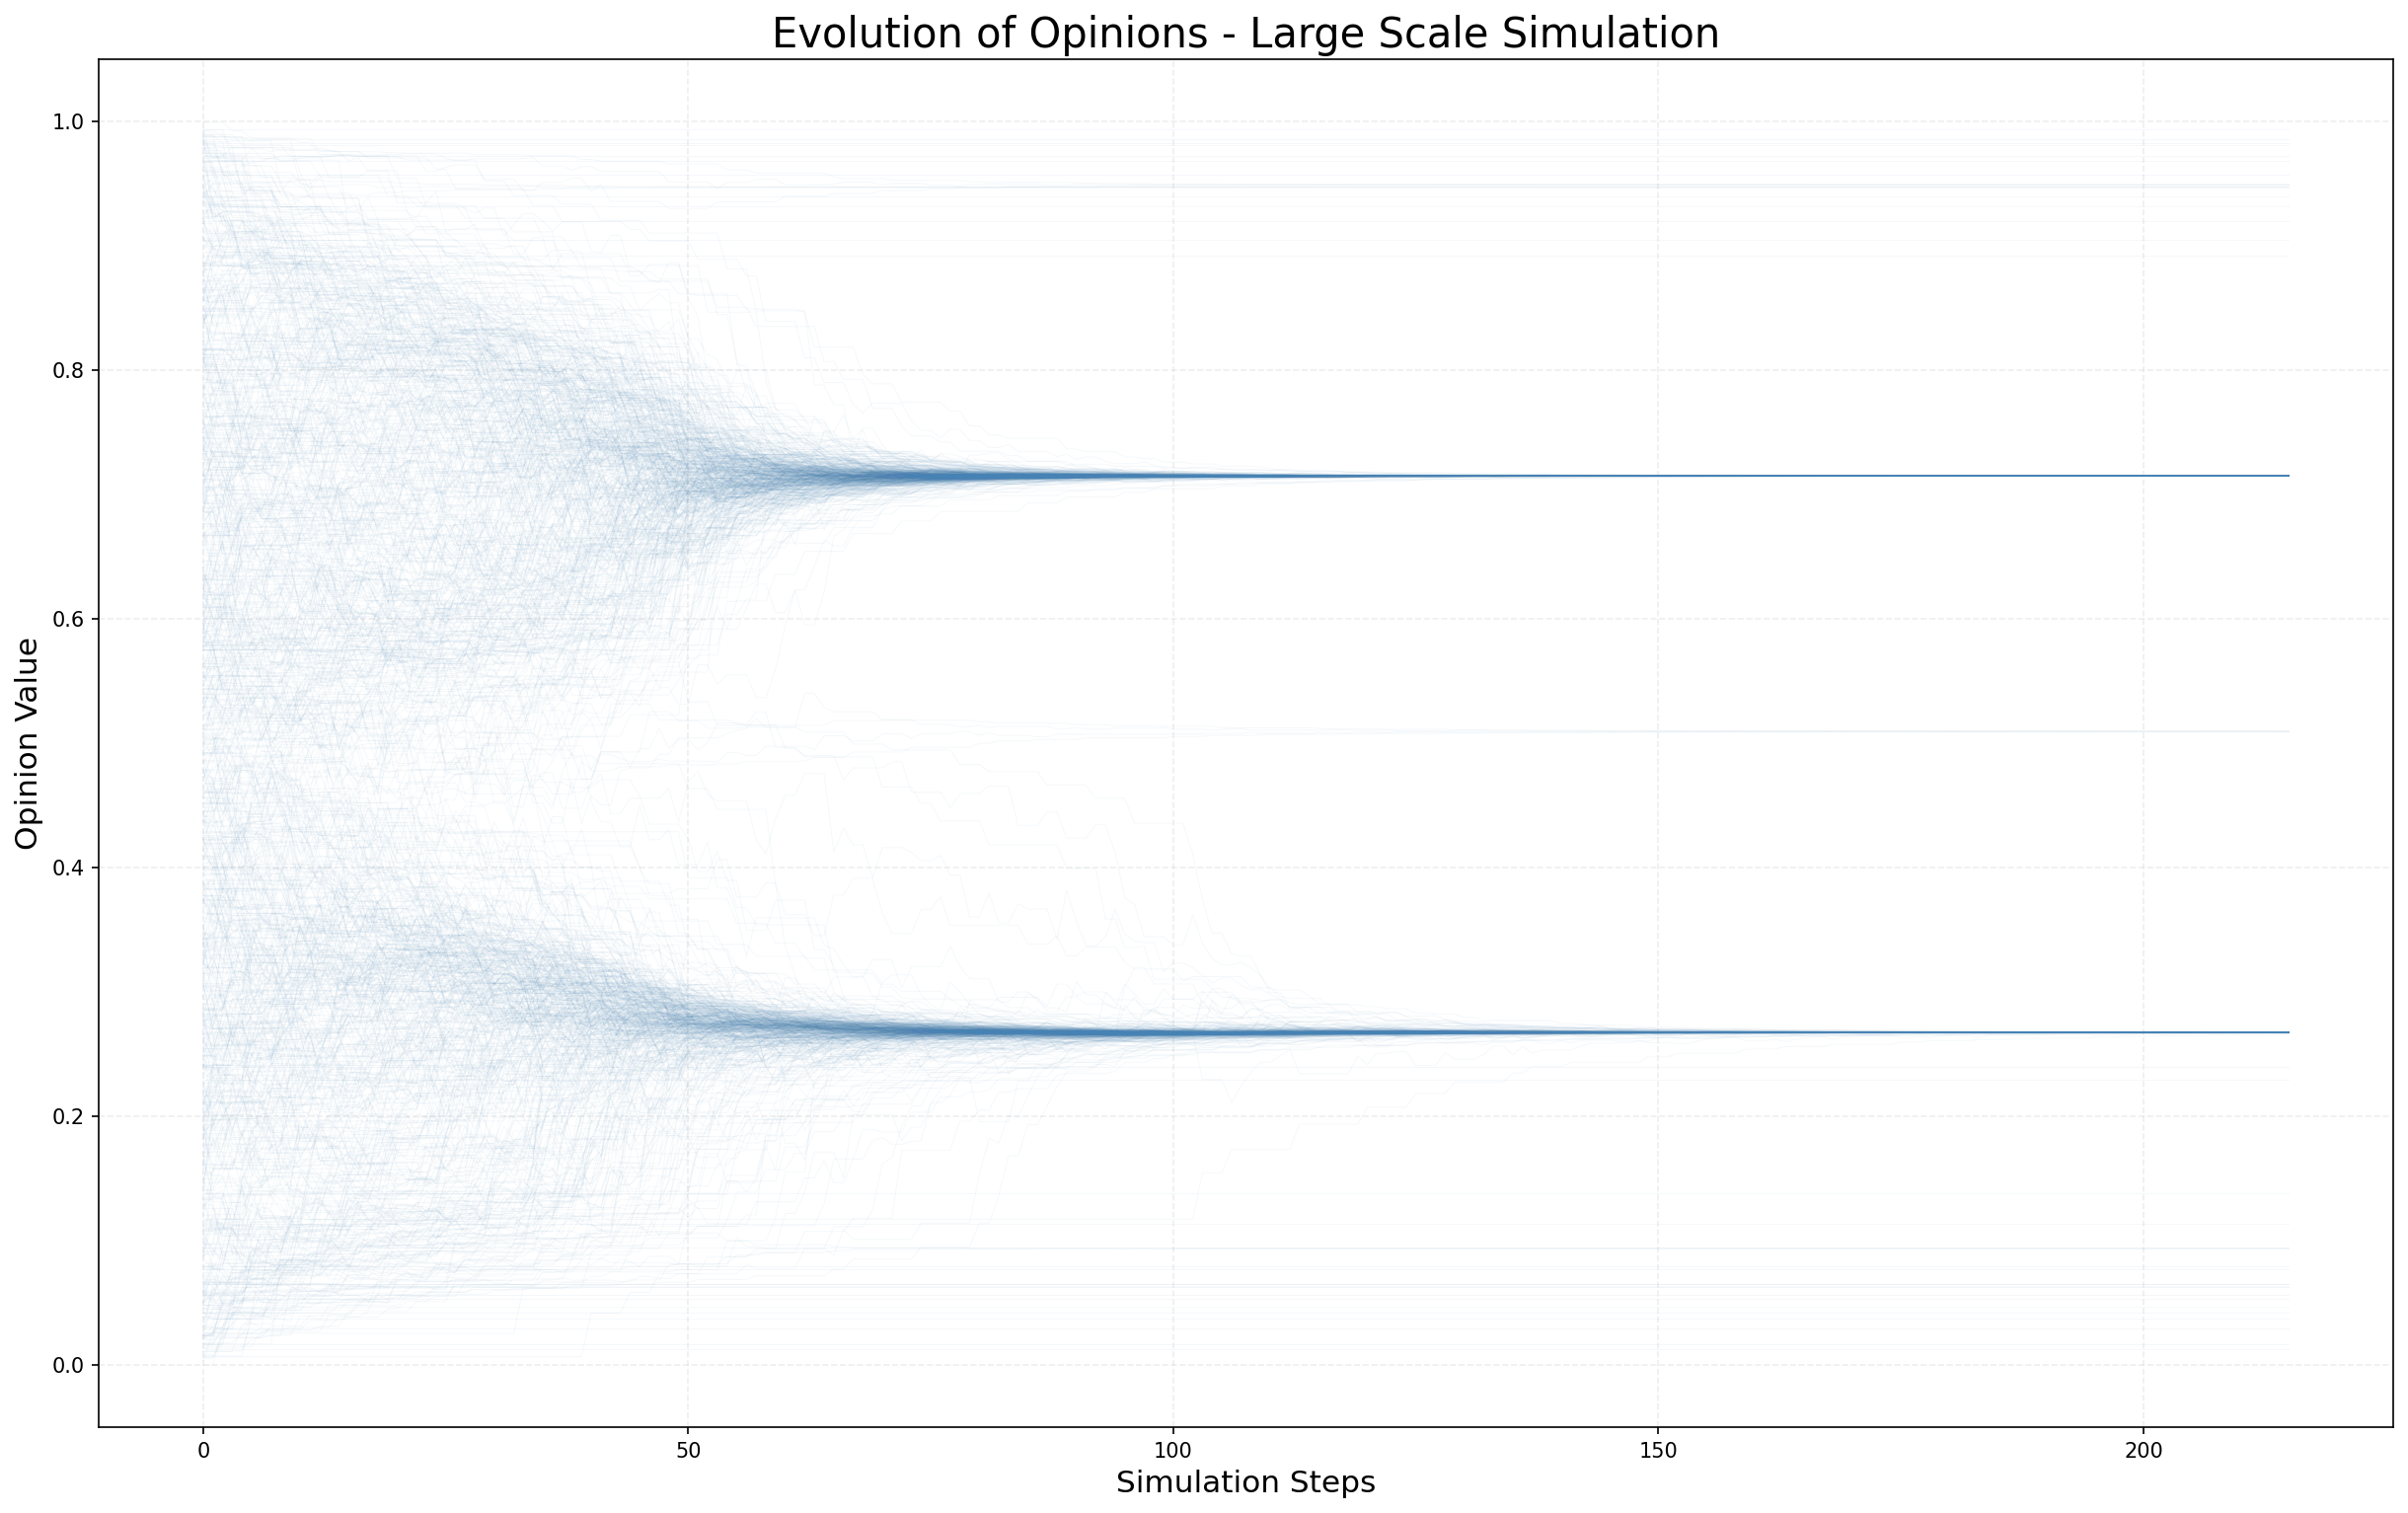
\includegraphics[width=\linewidth]{results/p_0.3_threshold_0.15/opinions_history_1}
            \caption{Polarización}
            \label{fig:p_0.3_threshold_0.15_1}
        \end{subfigure}
        \begin{subfigure}[b]{0.32\linewidth}
            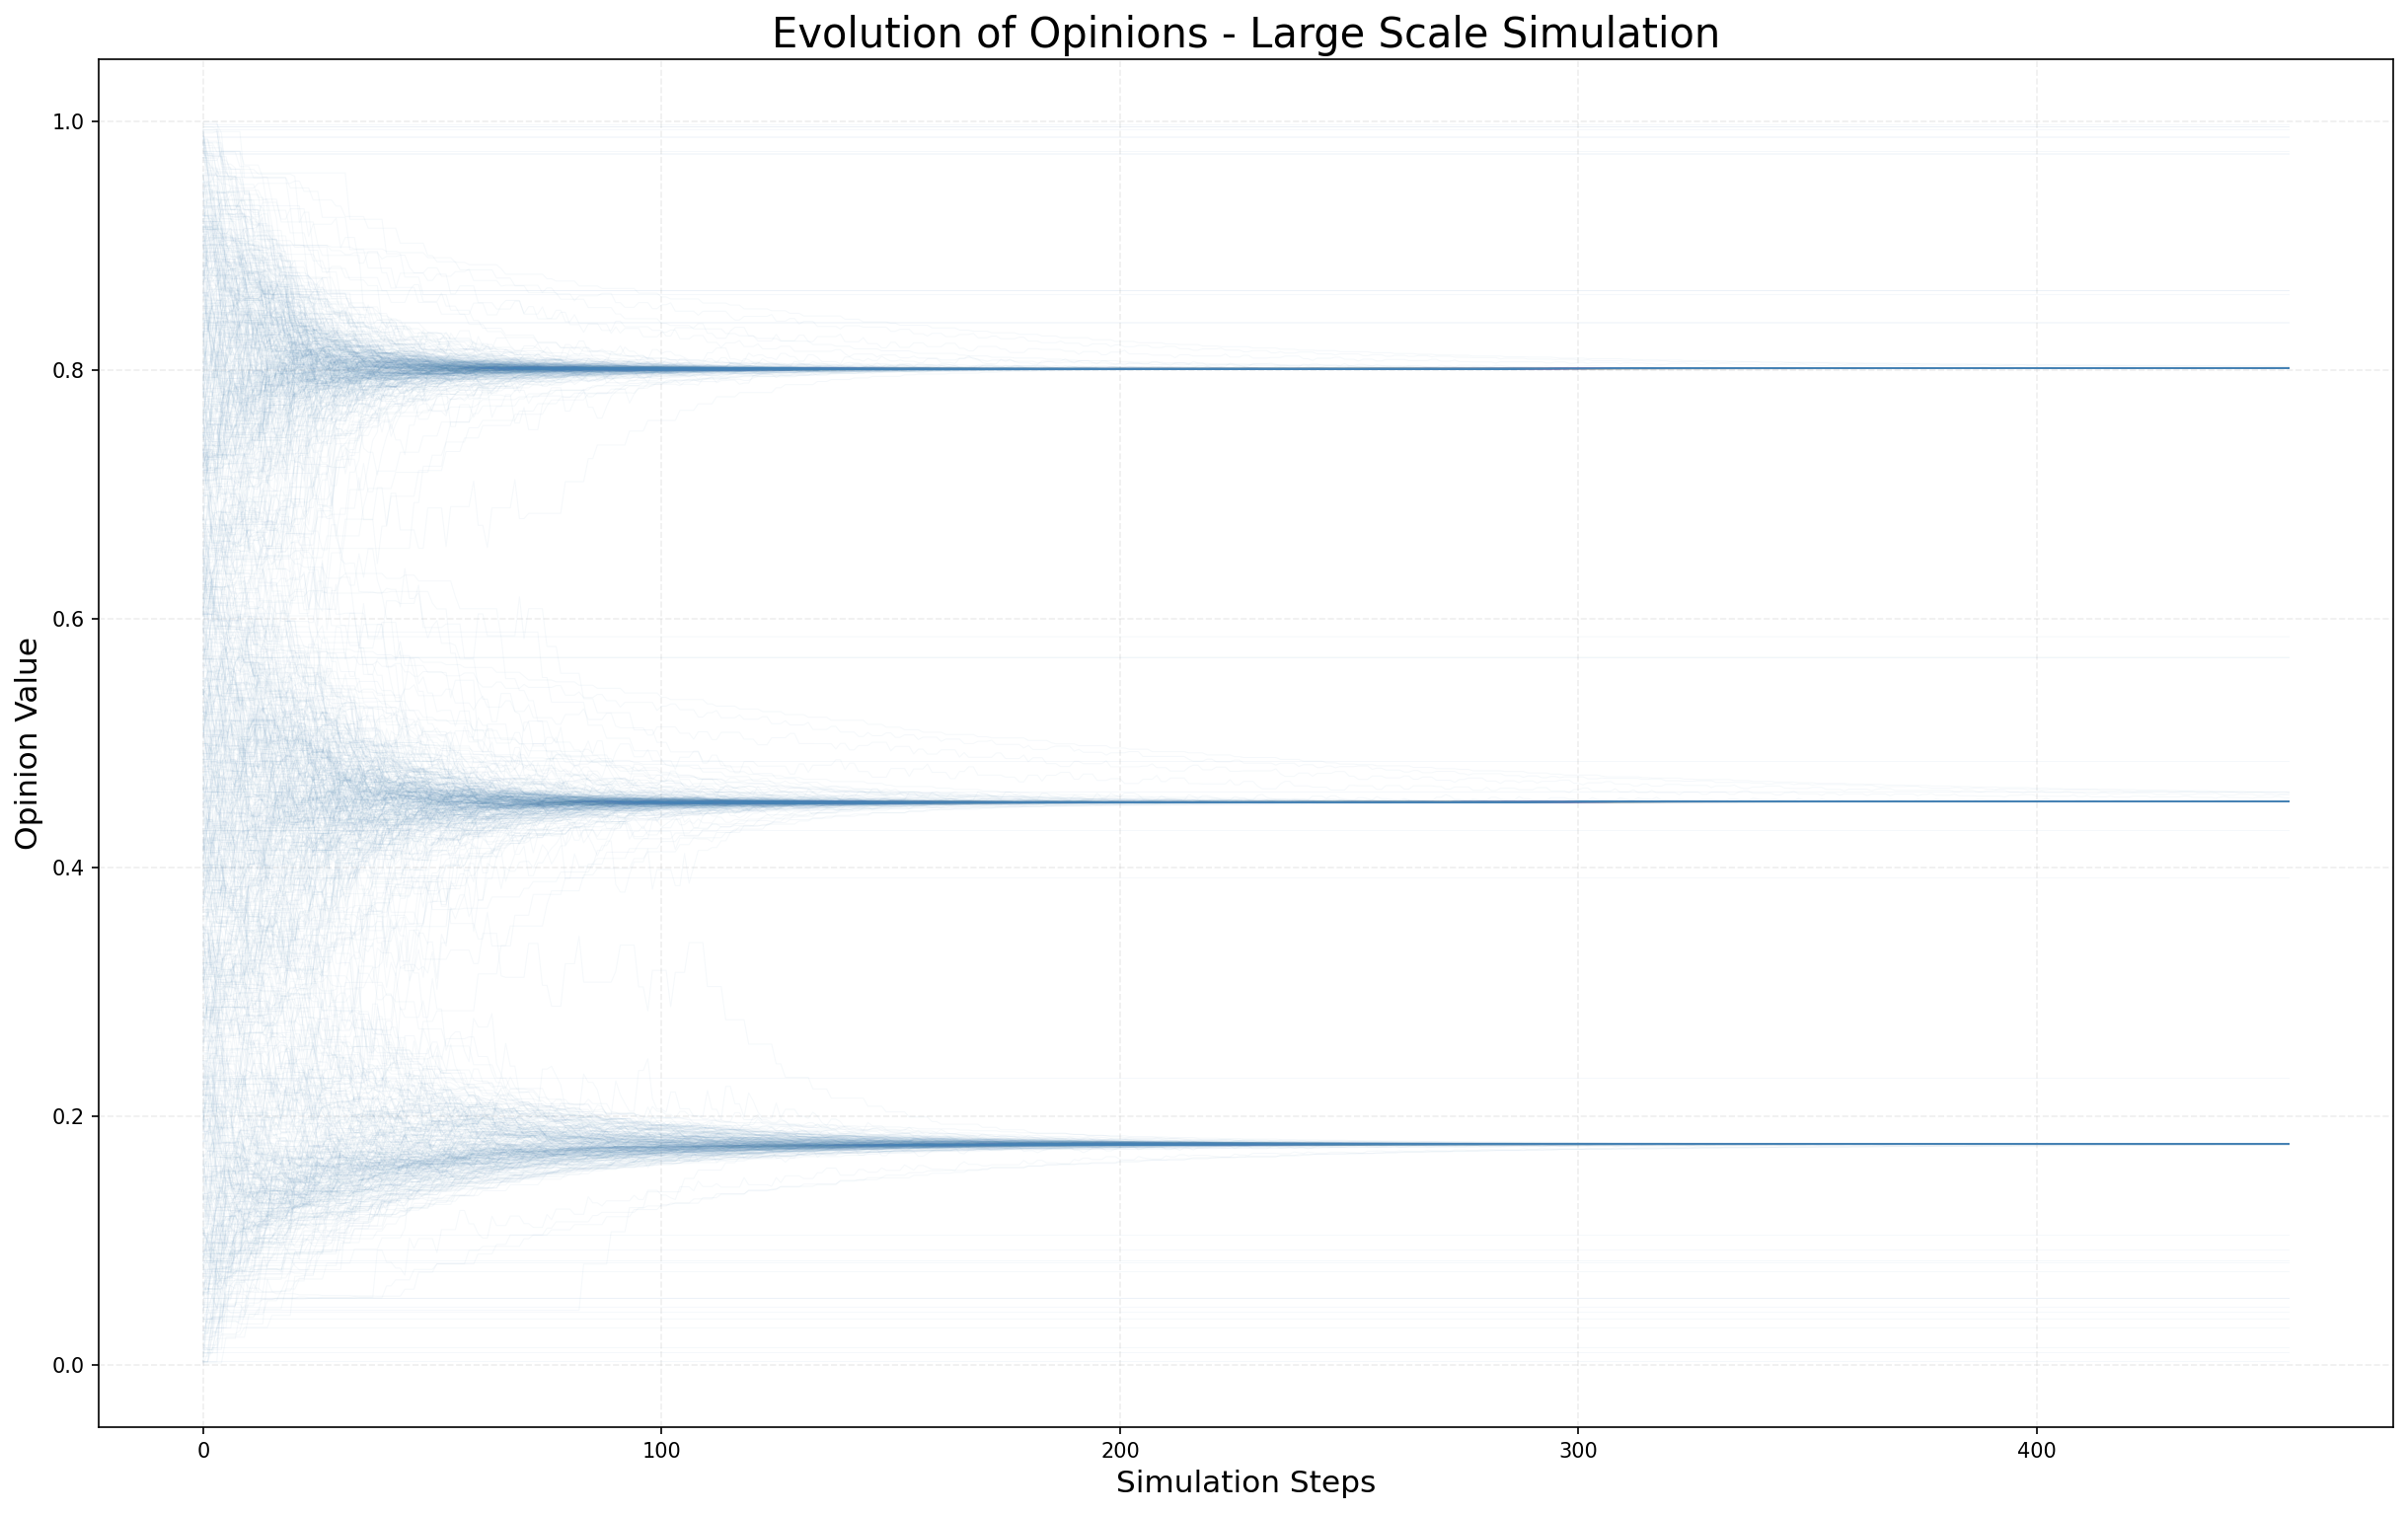
\includegraphics[width=\linewidth]{results/p_0.3_threshold_0.15/opinions_history_2}
            \caption{Fragmentación}
            \label{fig:p_0.3_threshold_0.15_2}
        \end{subfigure}
        \begin{subfigure}[b]{0.32\linewidth}
            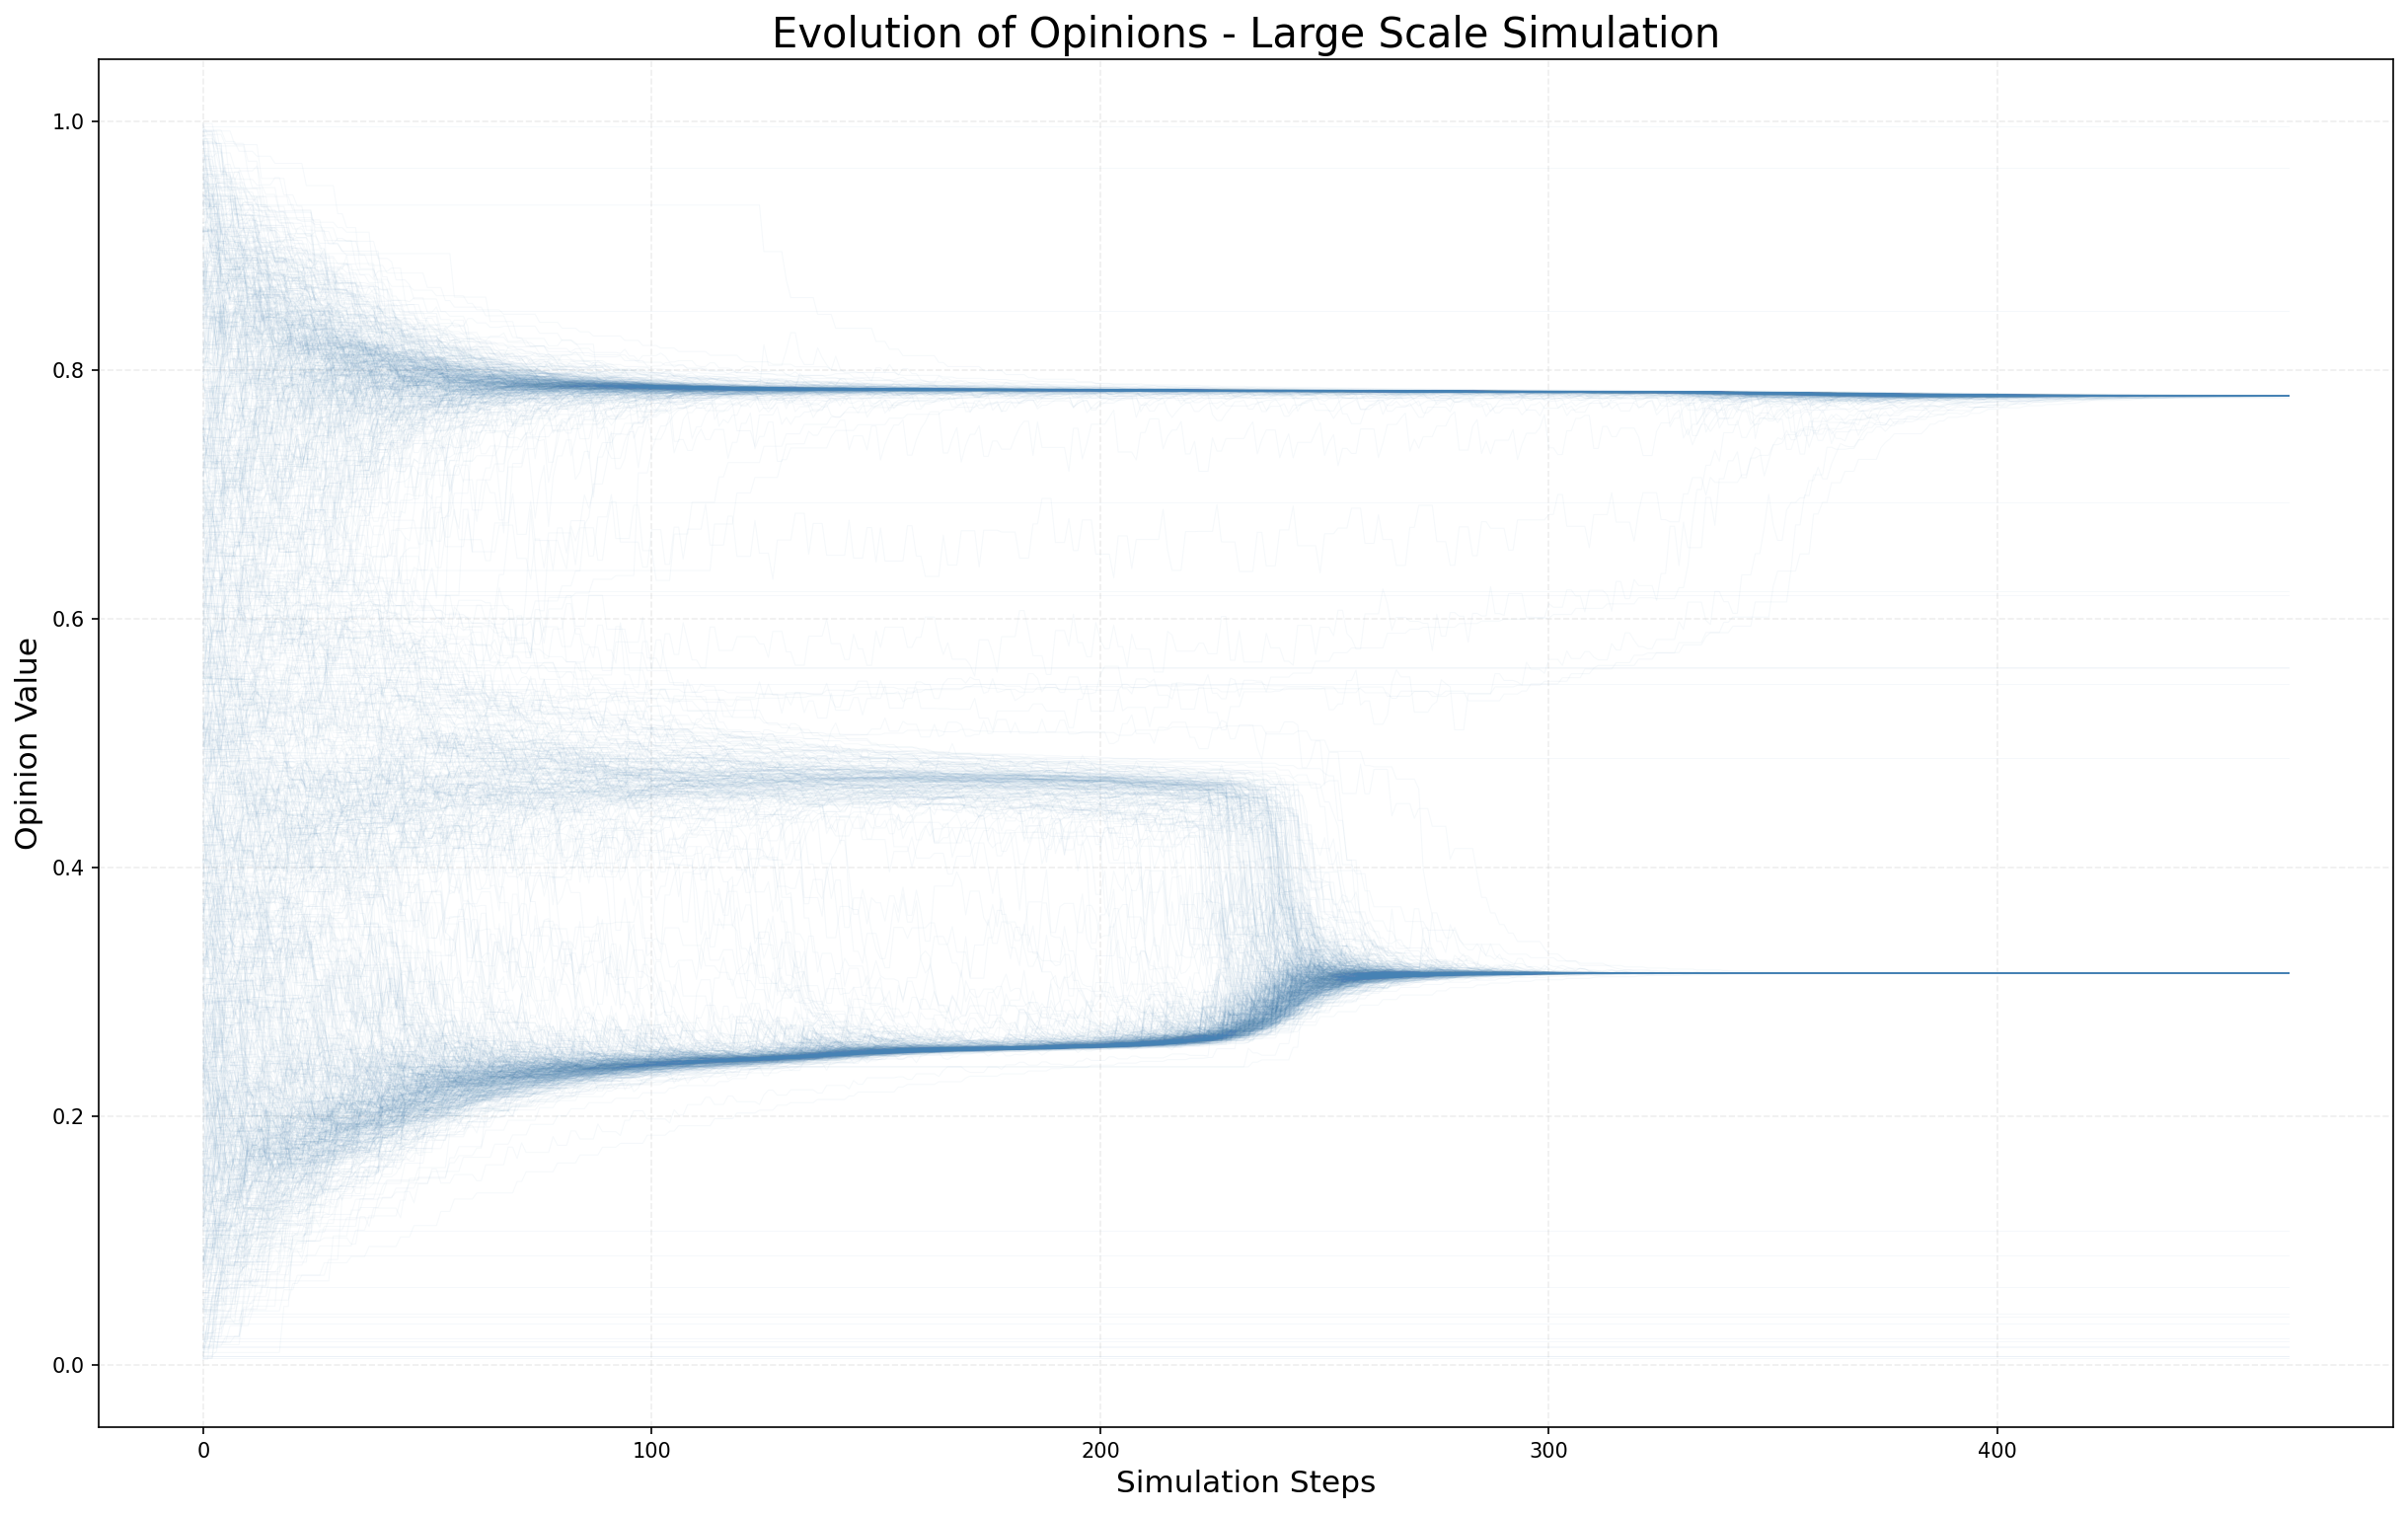
\includegraphics[width=\linewidth]{results/p_0.3_threshold_0.15/opinions_history_3}
            \caption{Fragmentación finalmente Polarización}
            \label{fig:p_0.3_threshold_0.15_3}
        \end{subfigure}
        \caption{Histórico de opiniones Prob. inter 0.3, confianza 0.15}
        \label{fig:p_0.3_threshold_0.15}
    \end{figure}
    \FloatBarrier



    \subsection{Prob. inter 0.3, confianza 0.2}
    \begin{figure}[htbp]
        \centering
        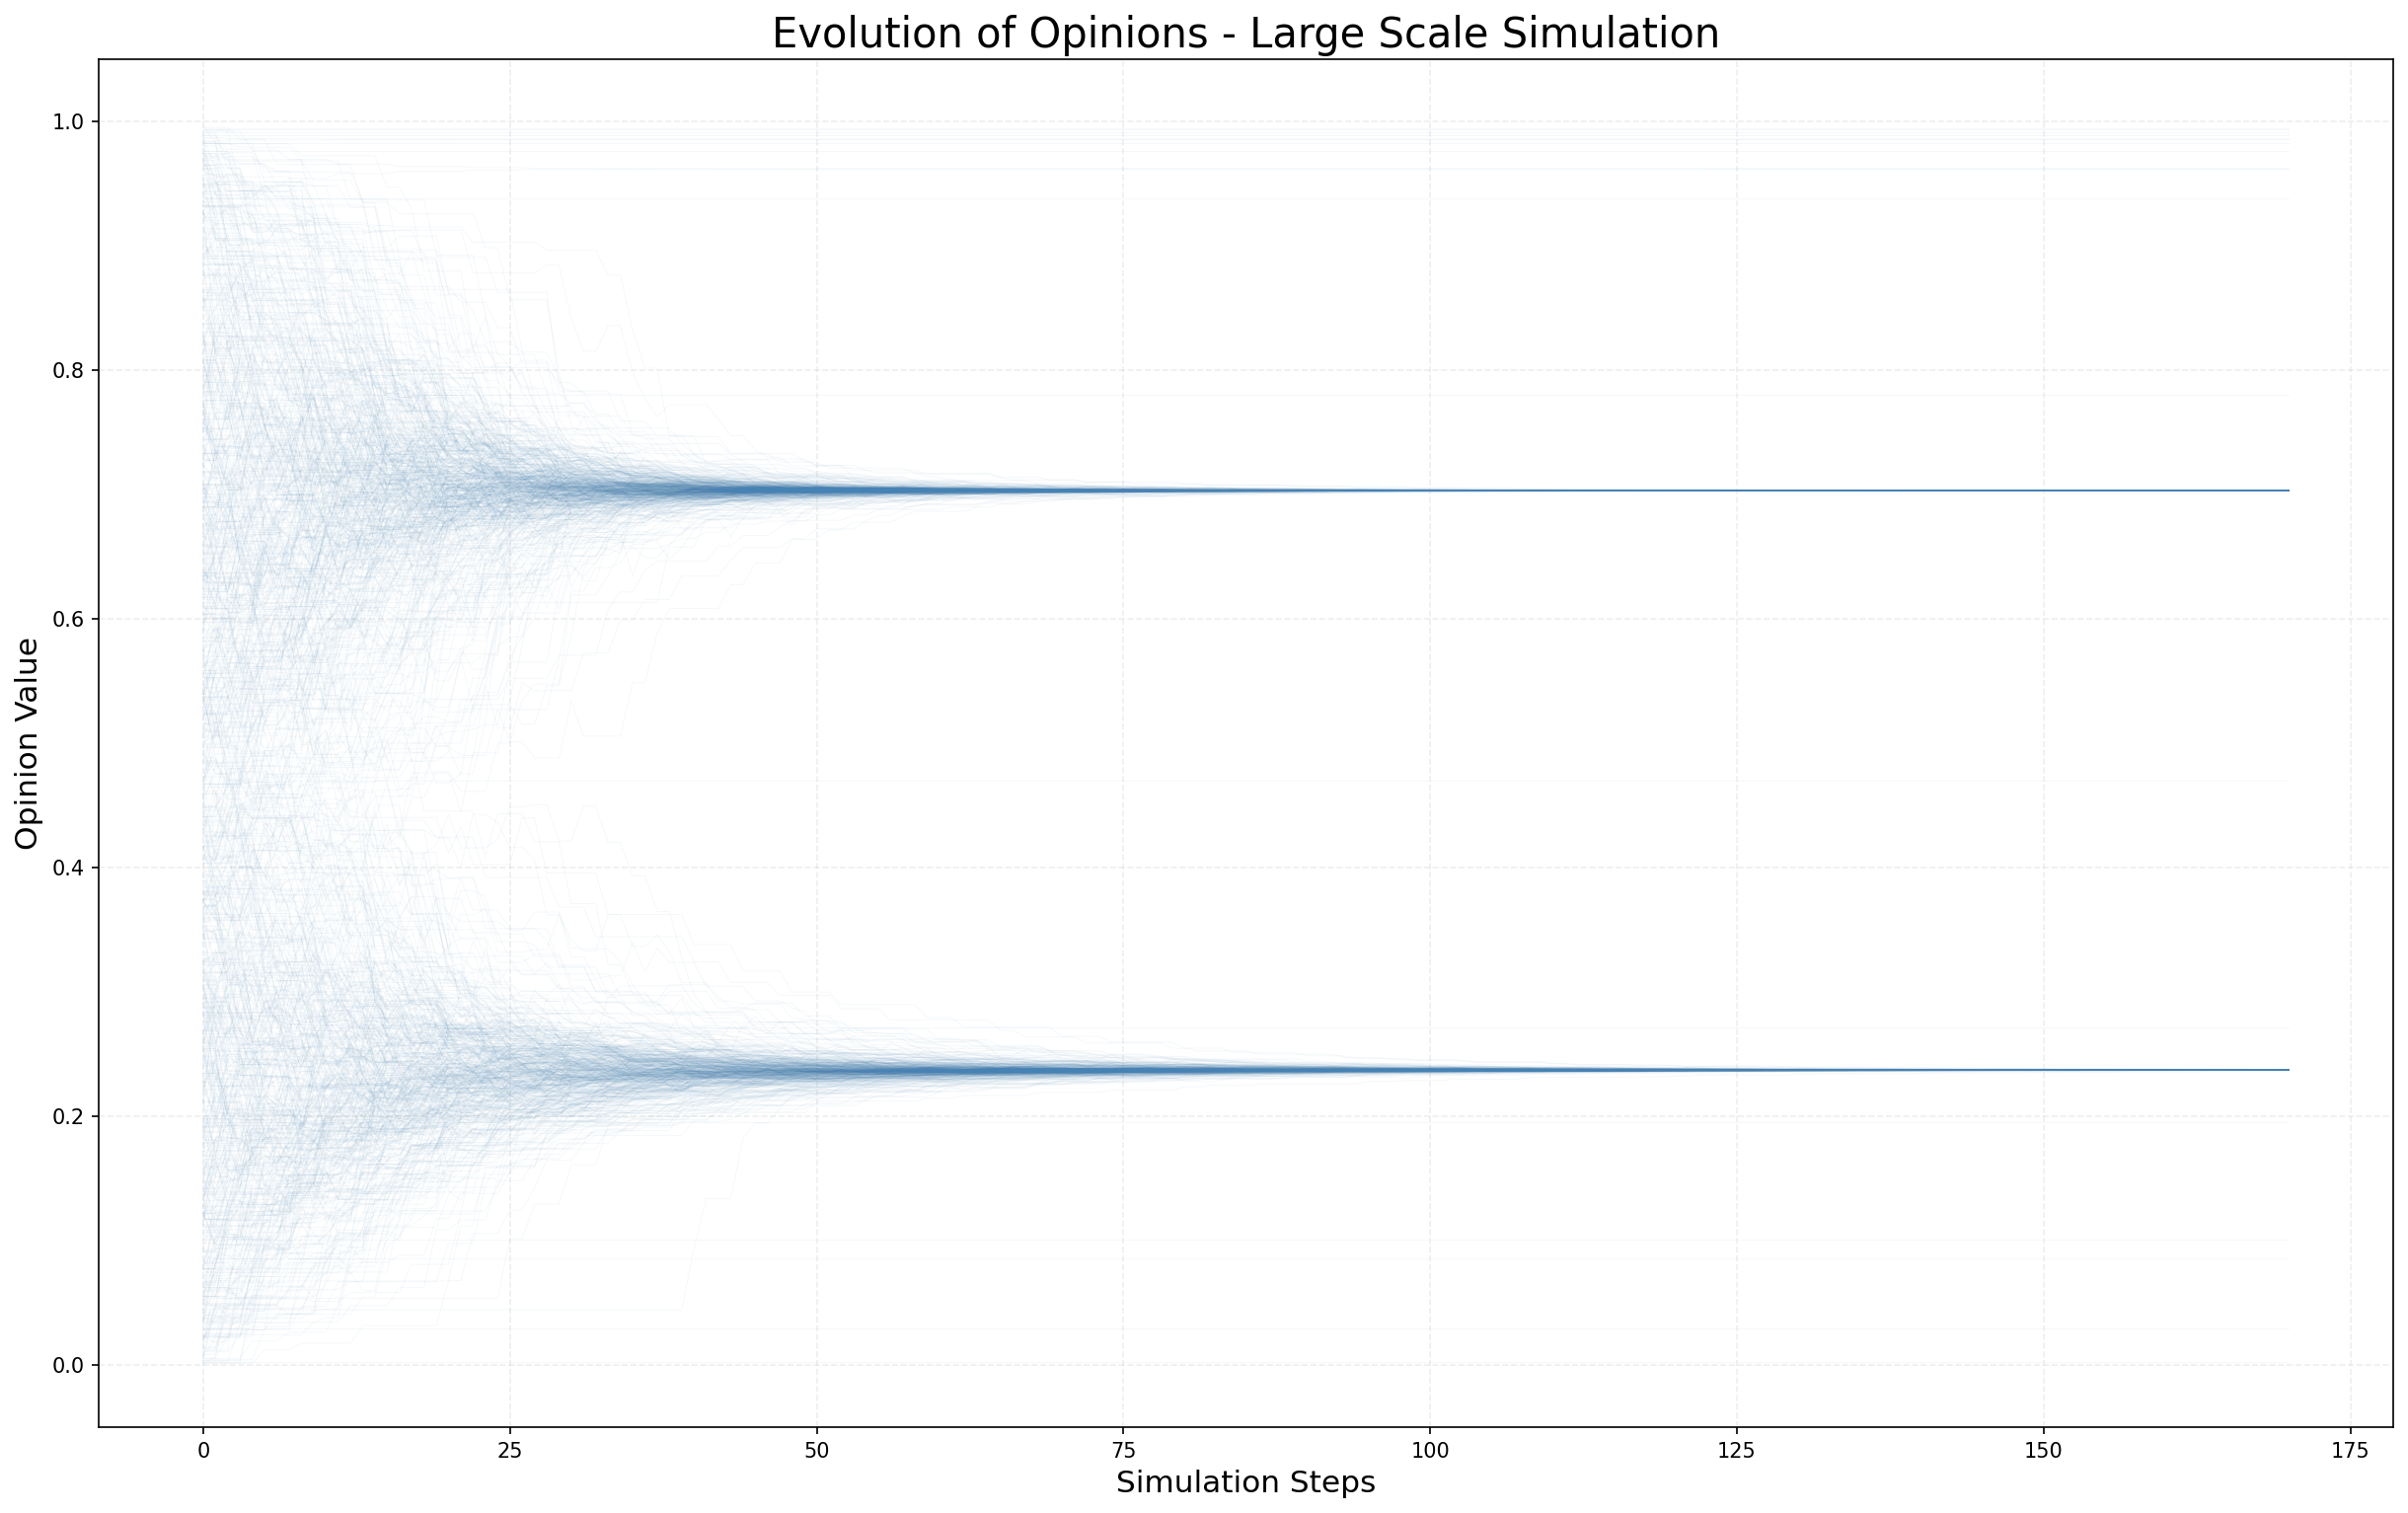
\includegraphics[width=0.33\linewidth]{results/p_0.3_threshold_0.2/opinions_history}
        \caption{Histórico de opiniones Prob. inter 0.3, confianza 0.2: Polarización}
        \label{fig:p_0.3_threshold_0.2}
    \end{figure}
    \FloatBarrier

    \subsection{Prob. inter 0.3, confianza 0.25}
    \begin{figure}[htbp]
        \centering
        \begin{subfigure}[b]{0.32\linewidth}
            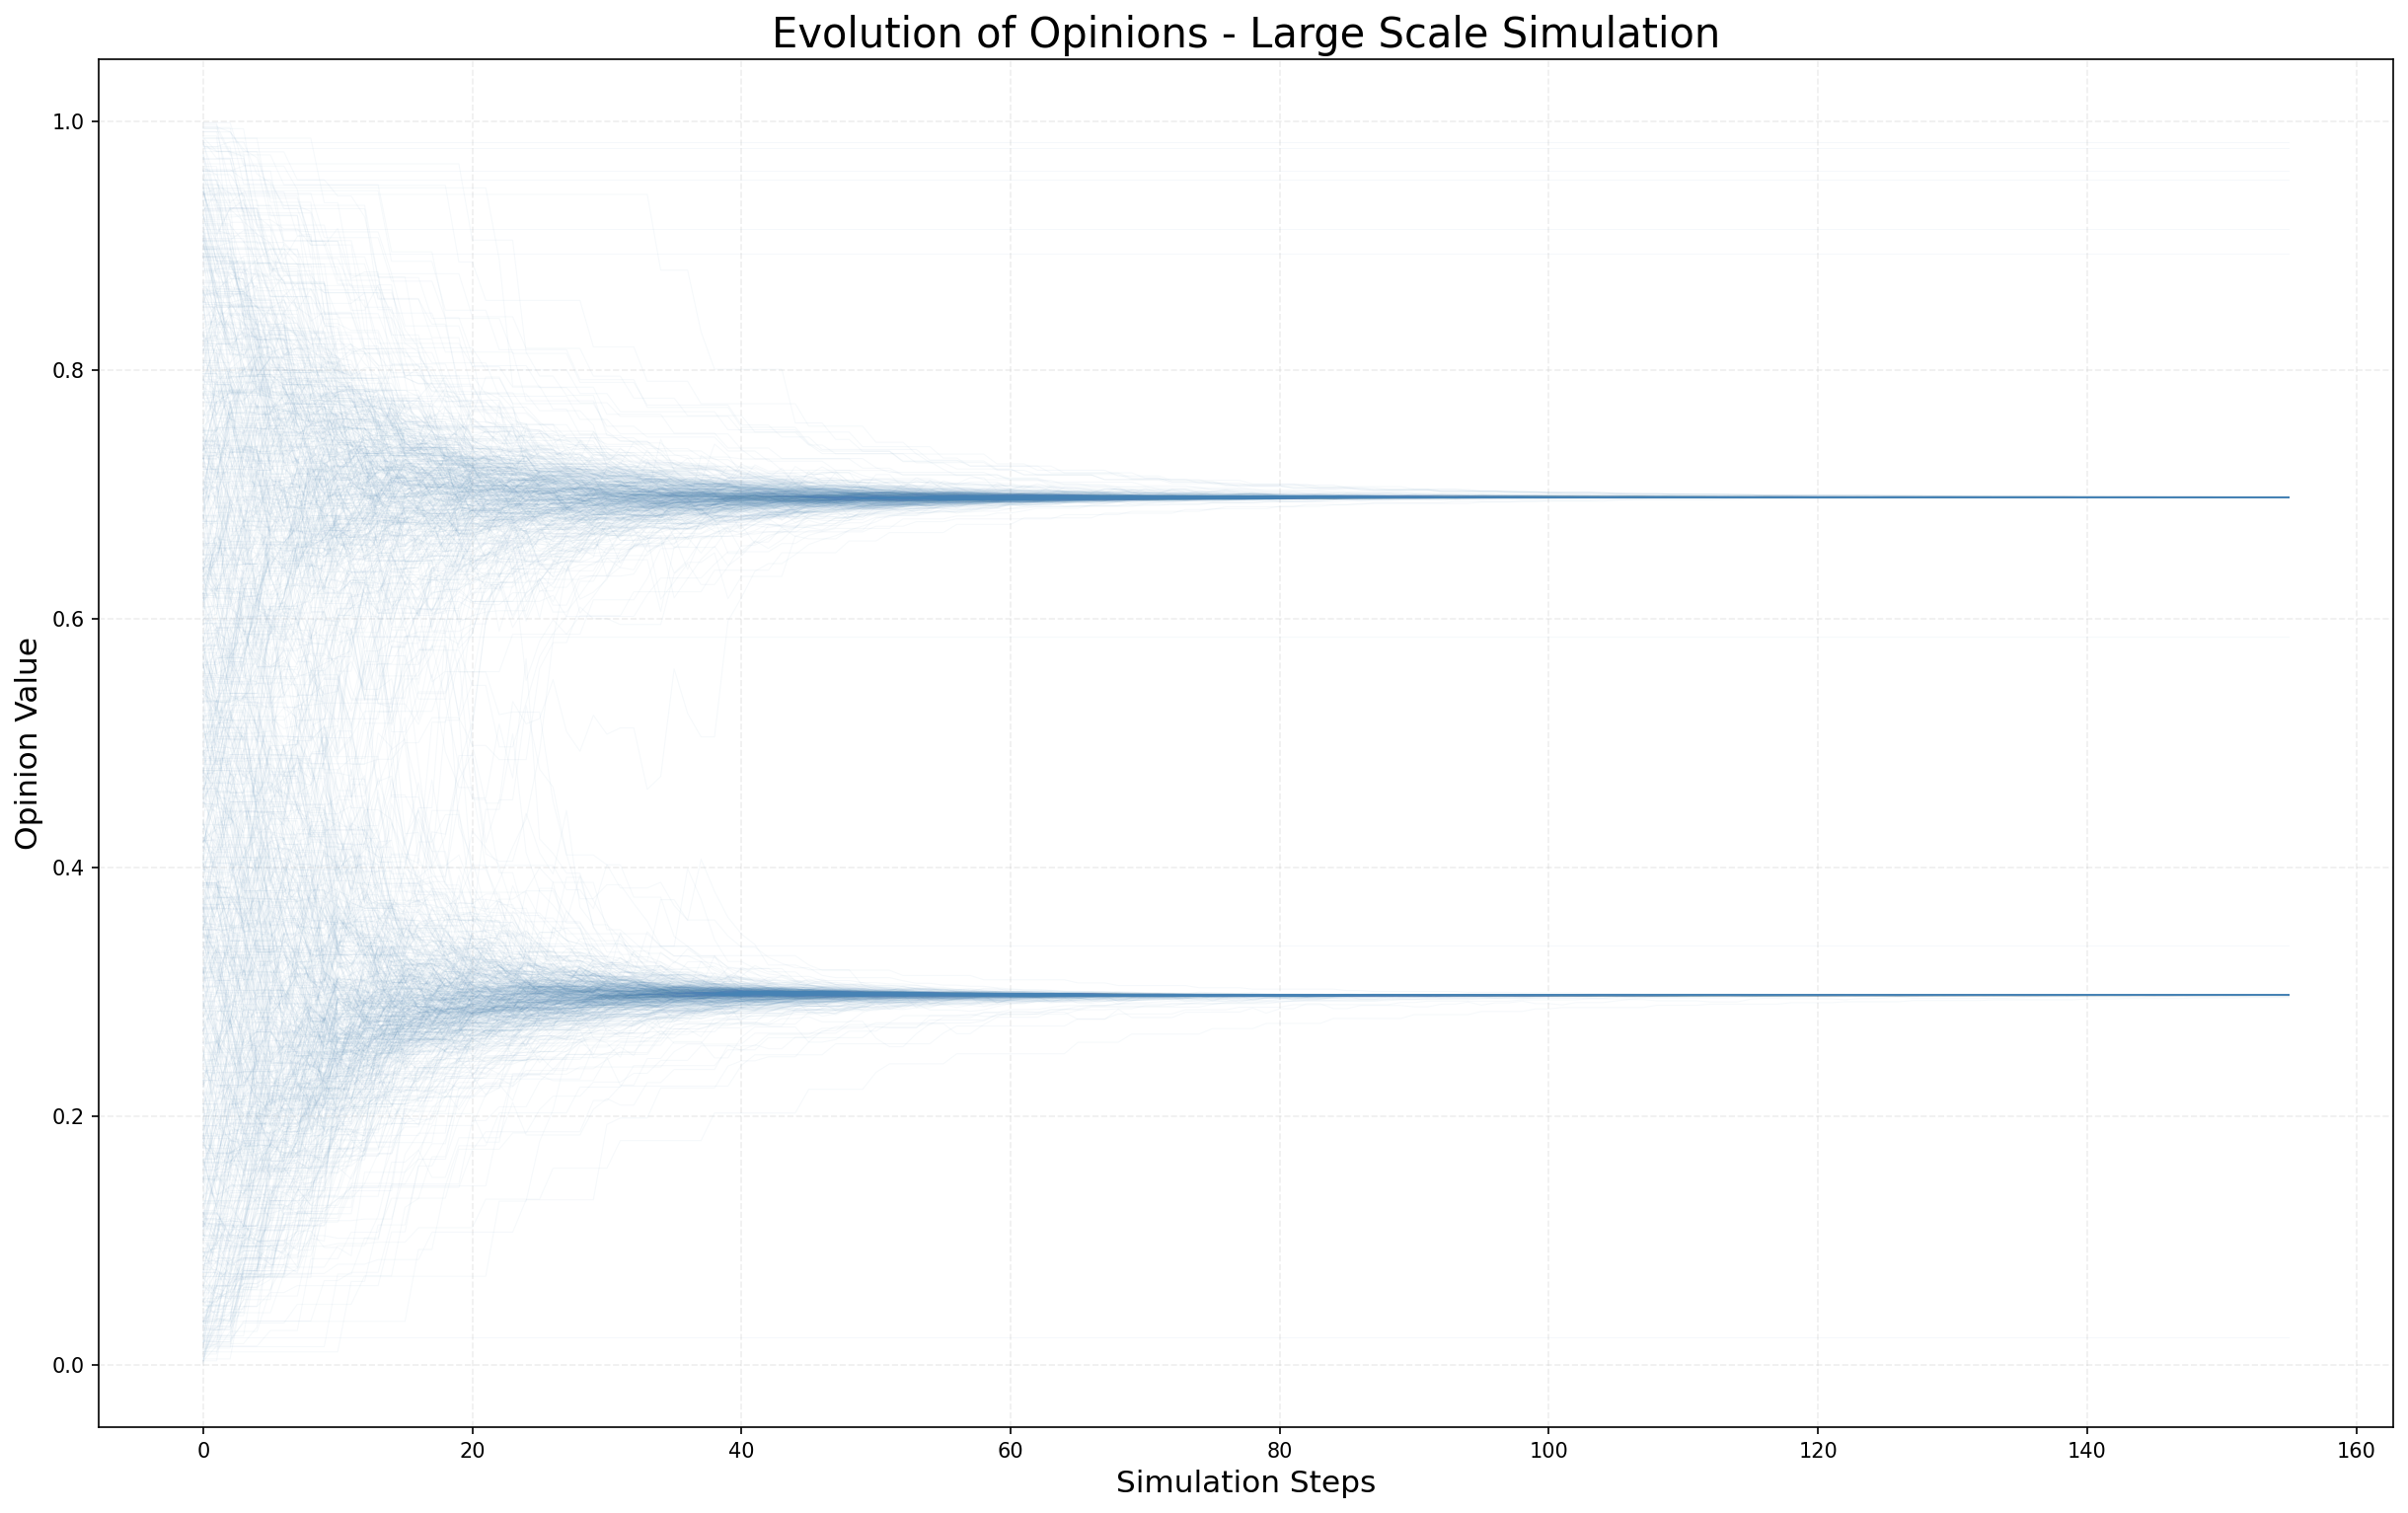
\includegraphics[width=\linewidth]{results/p_0.3_threshold_0.25/opinions_history_1}
            \caption{Polarización}
            \label{fig:p_0.3_threshold_0.25_1}
        \end{subfigure}
        \begin{subfigure}[b]{0.32\linewidth}
            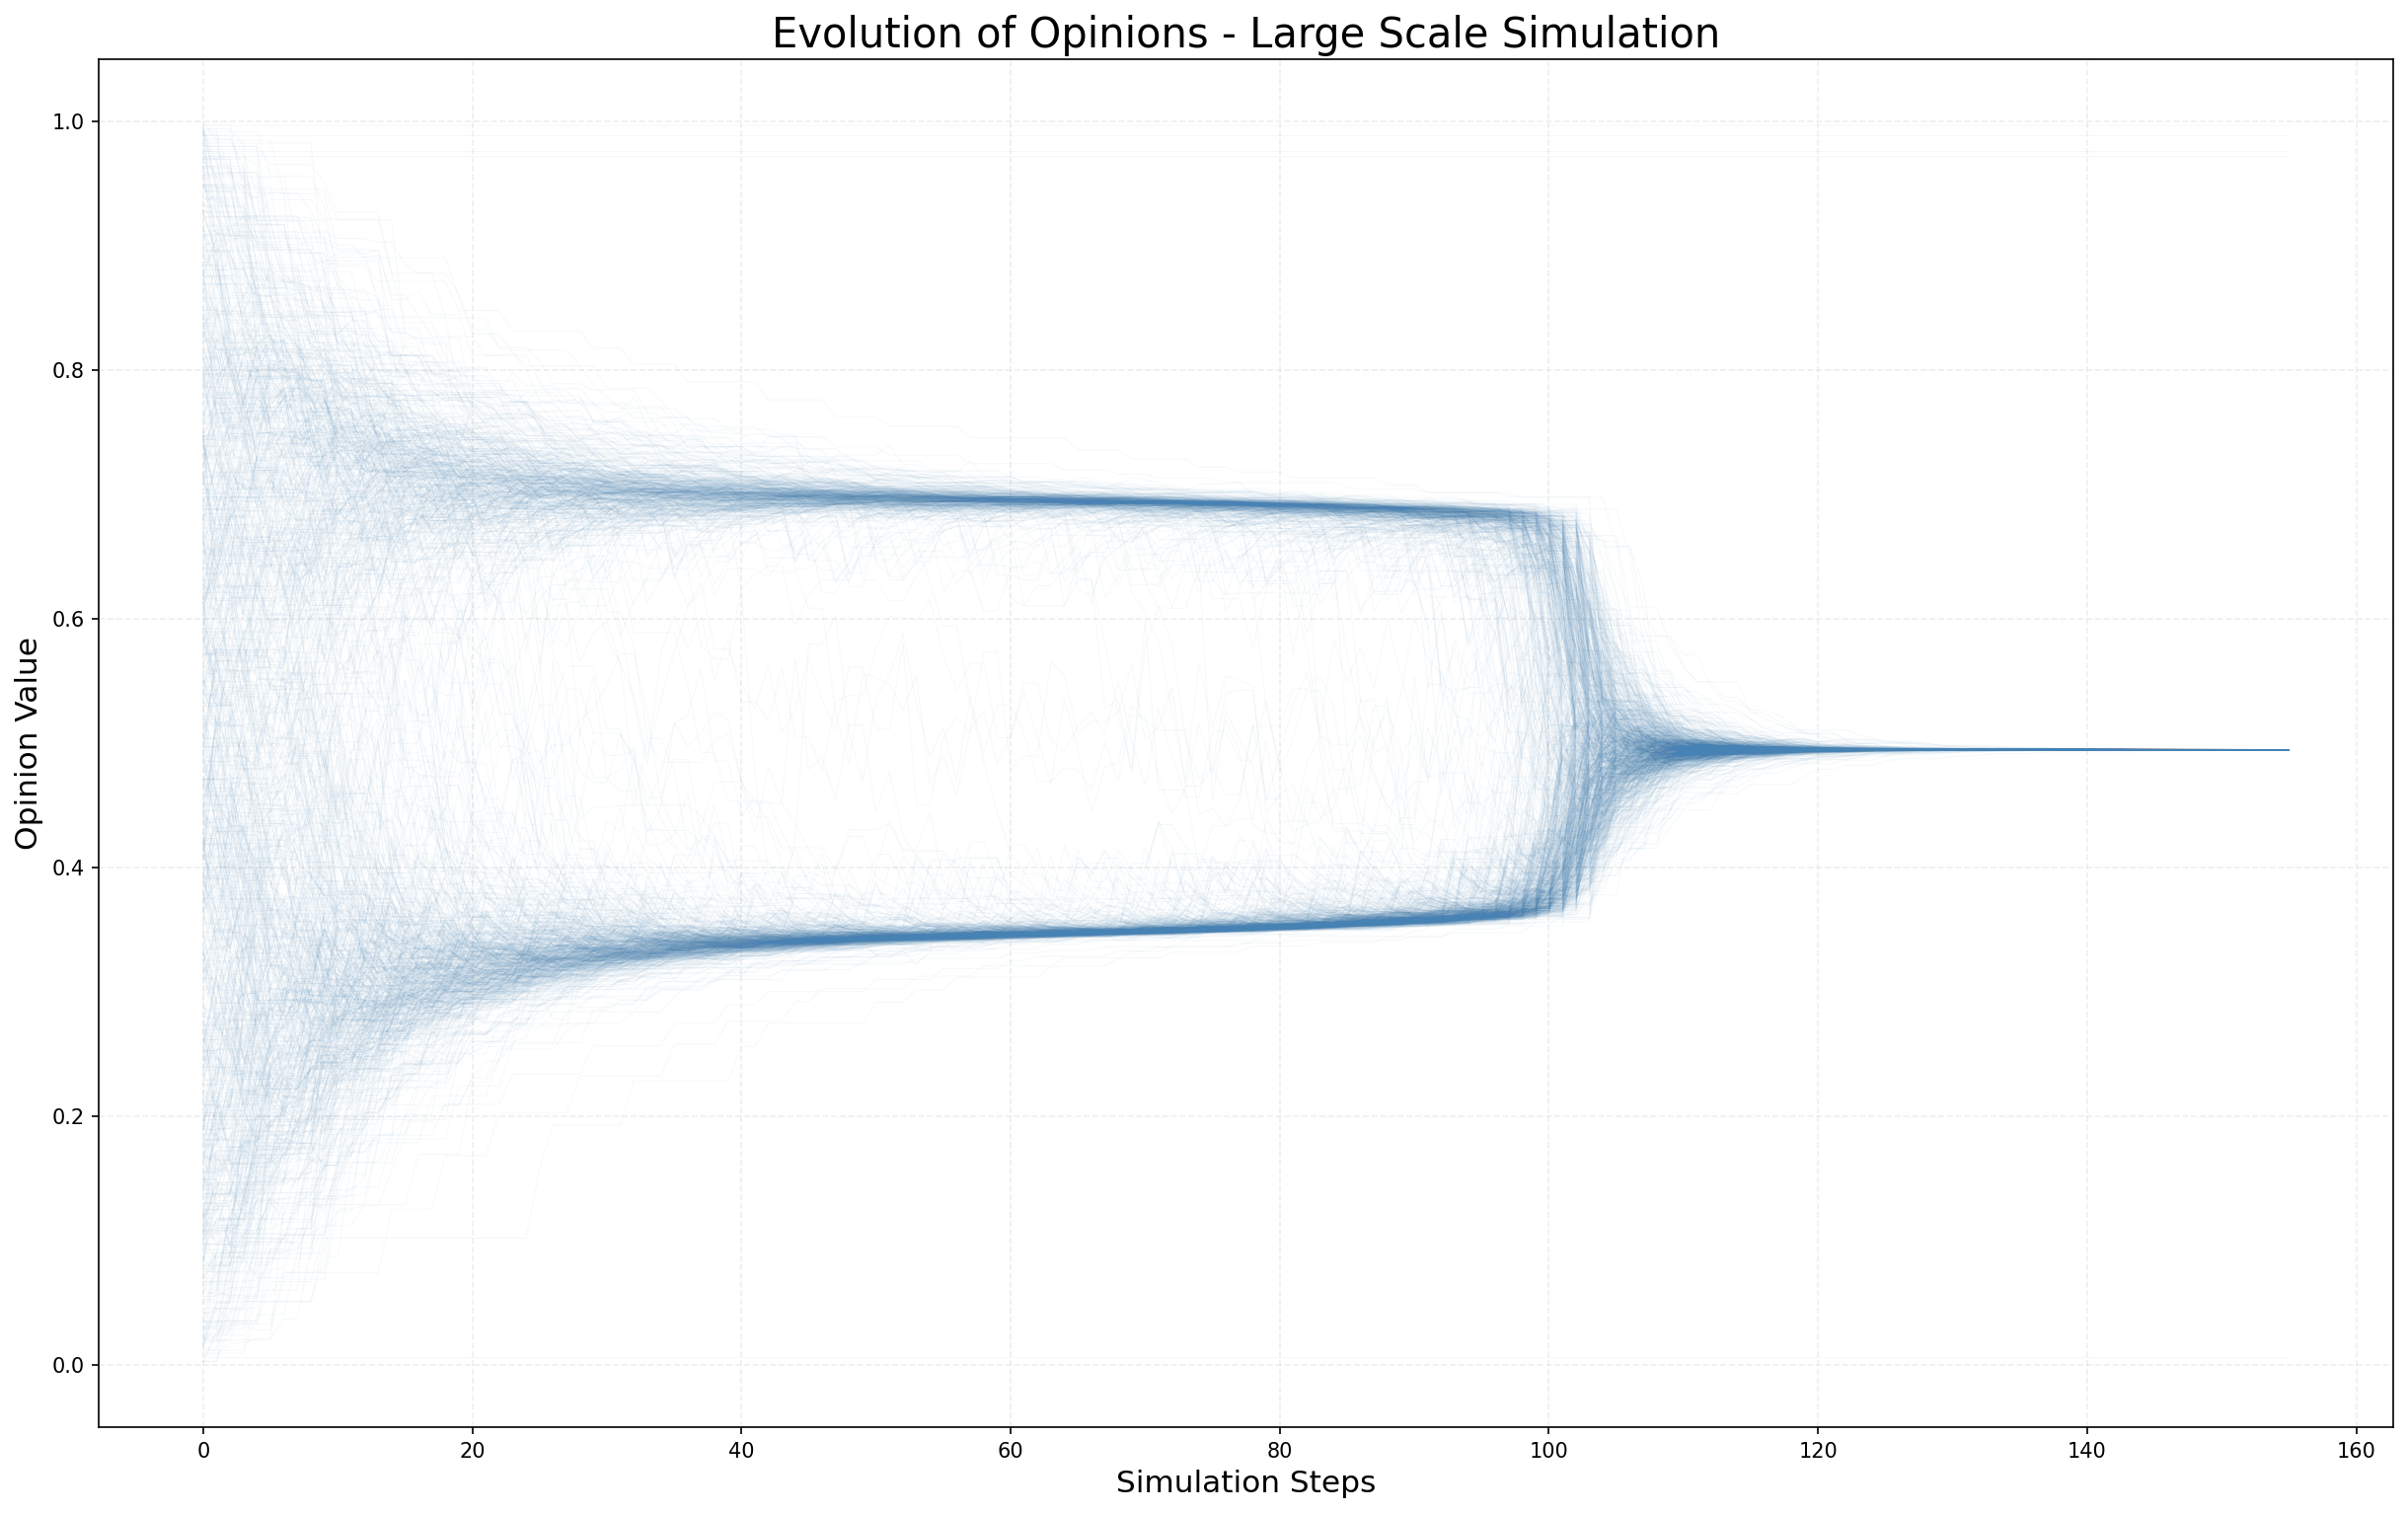
\includegraphics[width=\linewidth]{results/p_0.3_threshold_0.25/opinions_history_2}
            \caption{Polarización finalmente consenso}
            \label{fig:p_0.3_threshold_0.25_2}
        \end{subfigure}
        \begin{subfigure}[b]{0.32\linewidth}
            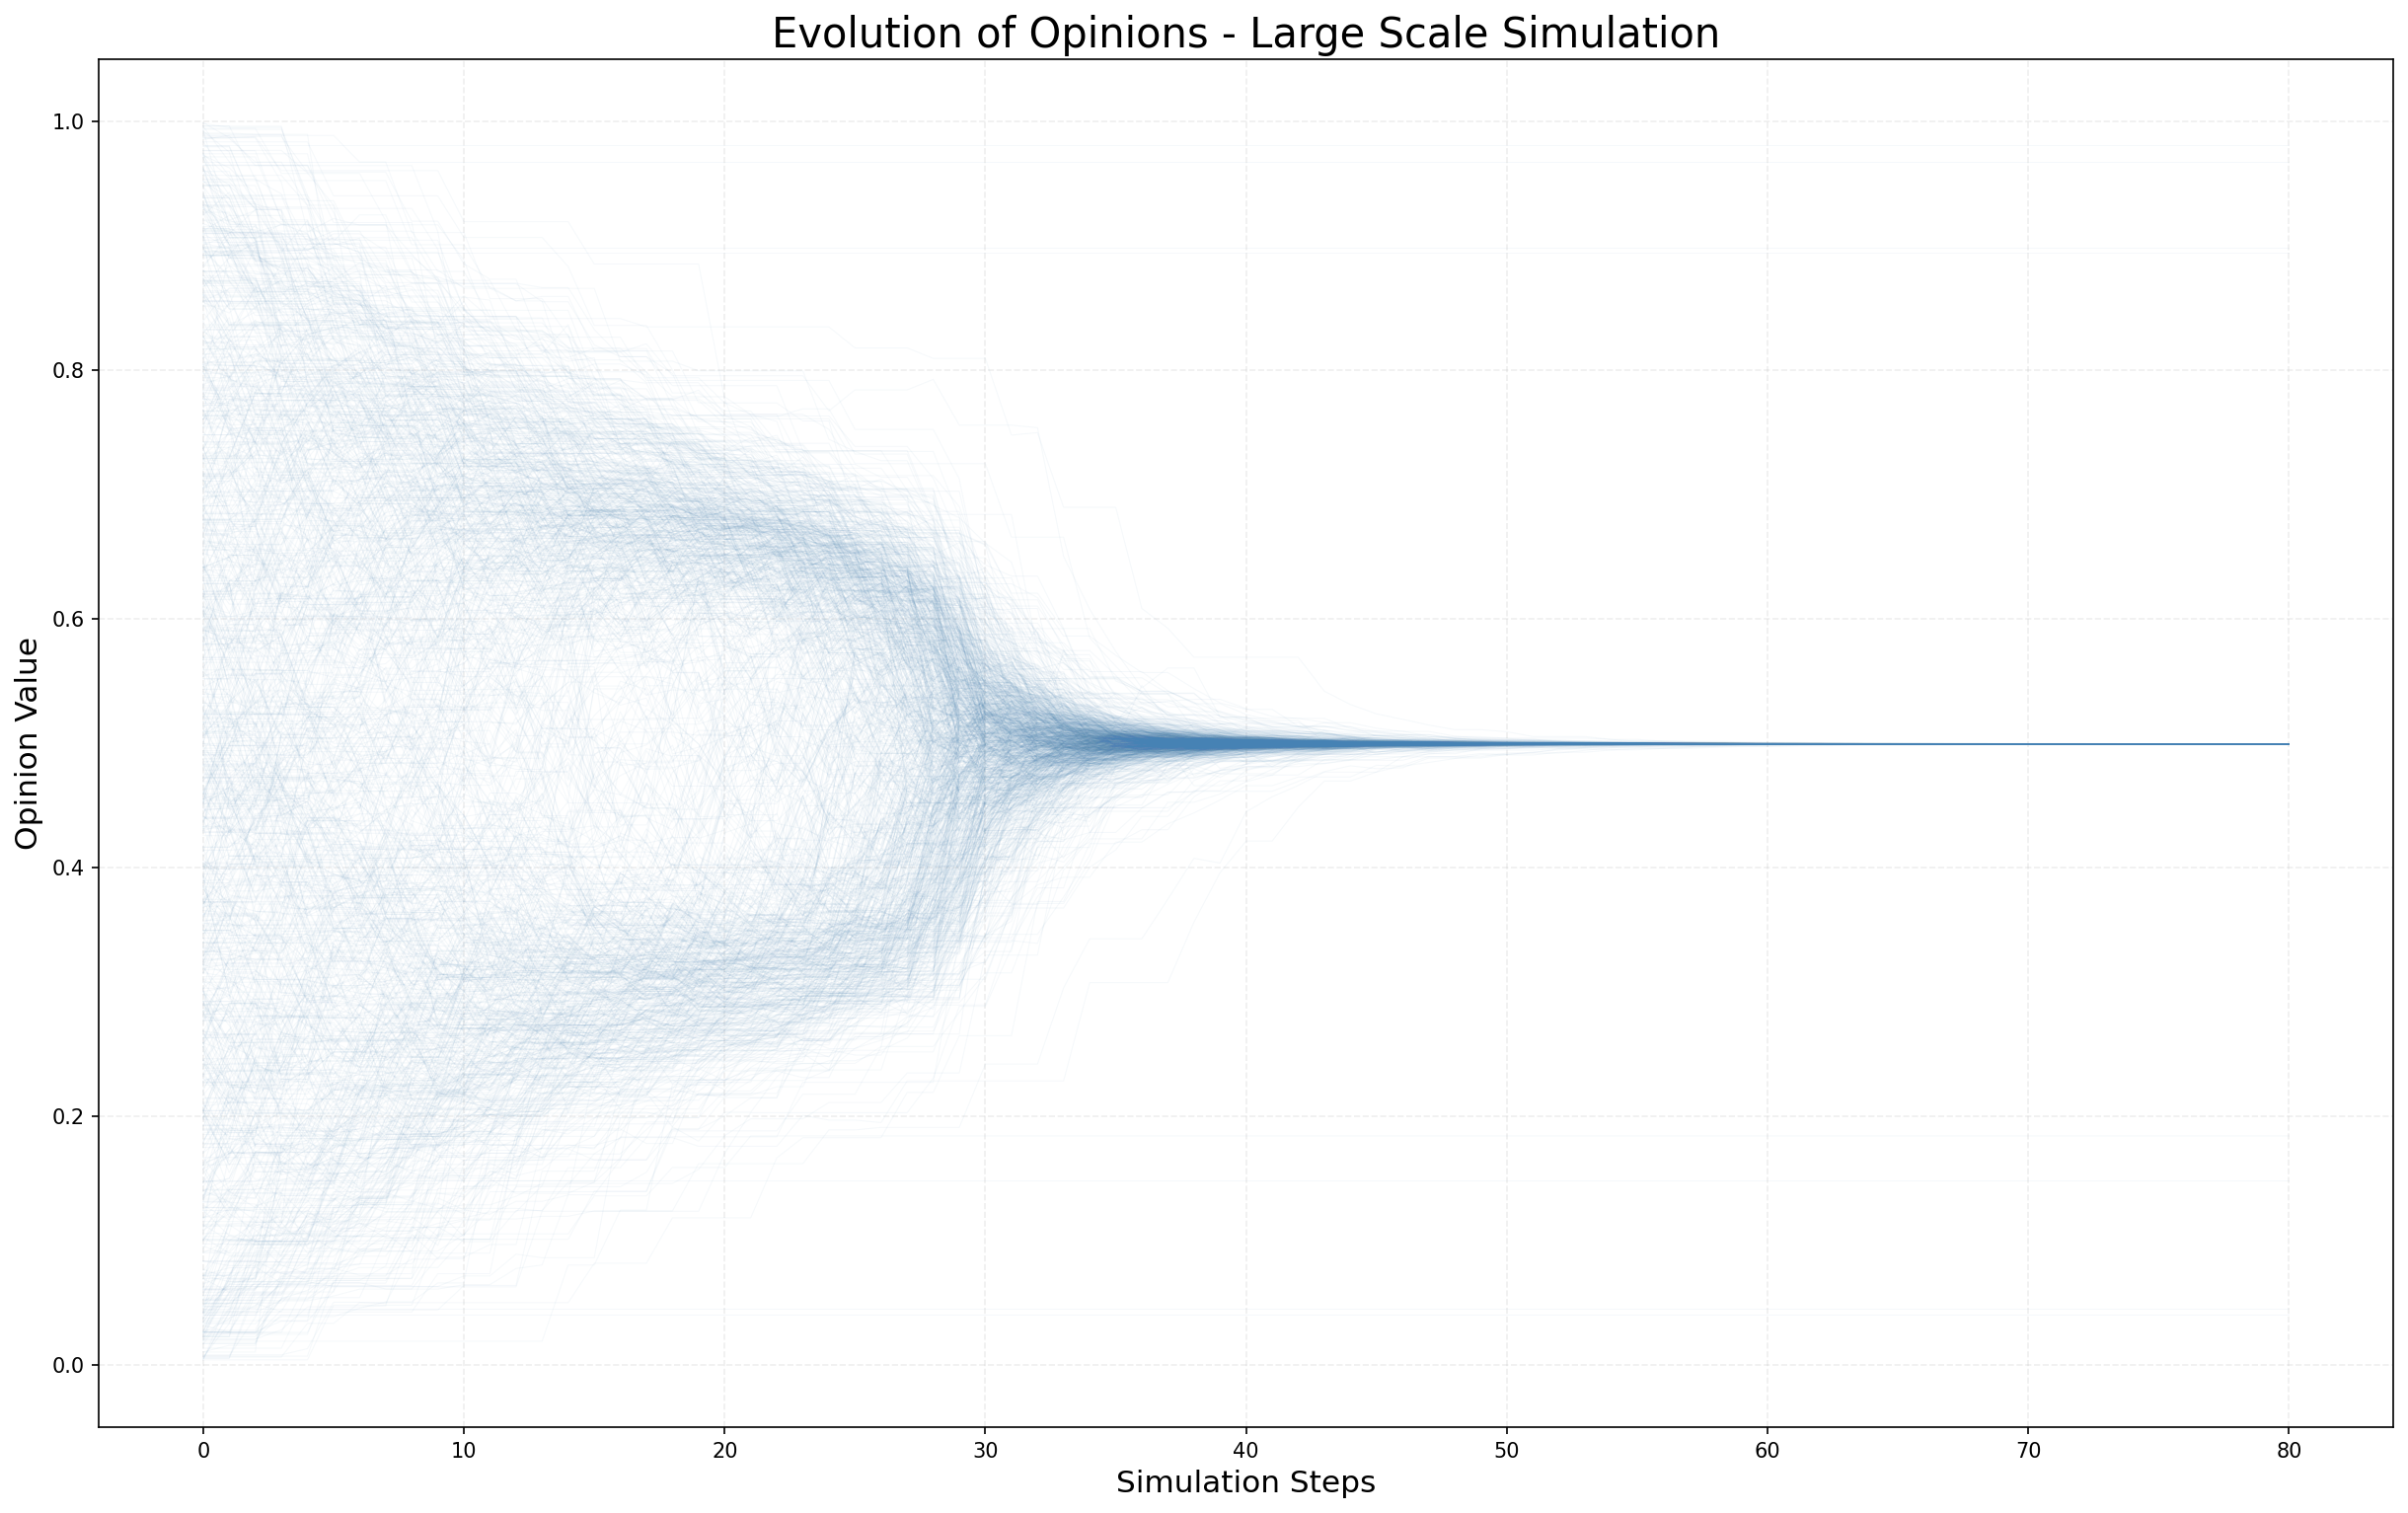
\includegraphics[width=\linewidth]{results/p_0.3_threshold_0.25/opinions_history_3}
            \caption{Polarización finalmente Consenso}
            \label{fig:p_0.3_threshold_0.25_3}
        \end{subfigure}
        \caption{Histórico de opiniones Prob. inter 0.3, confianza 0.25}
        \label{fig:p_0.3_threshold_0.25}
    \end{figure}
    \FloatBarrier

    \subsection{Prob. inter 0.3, confianza 0.3}
    \begin{figure}[htbp]
        \centering
        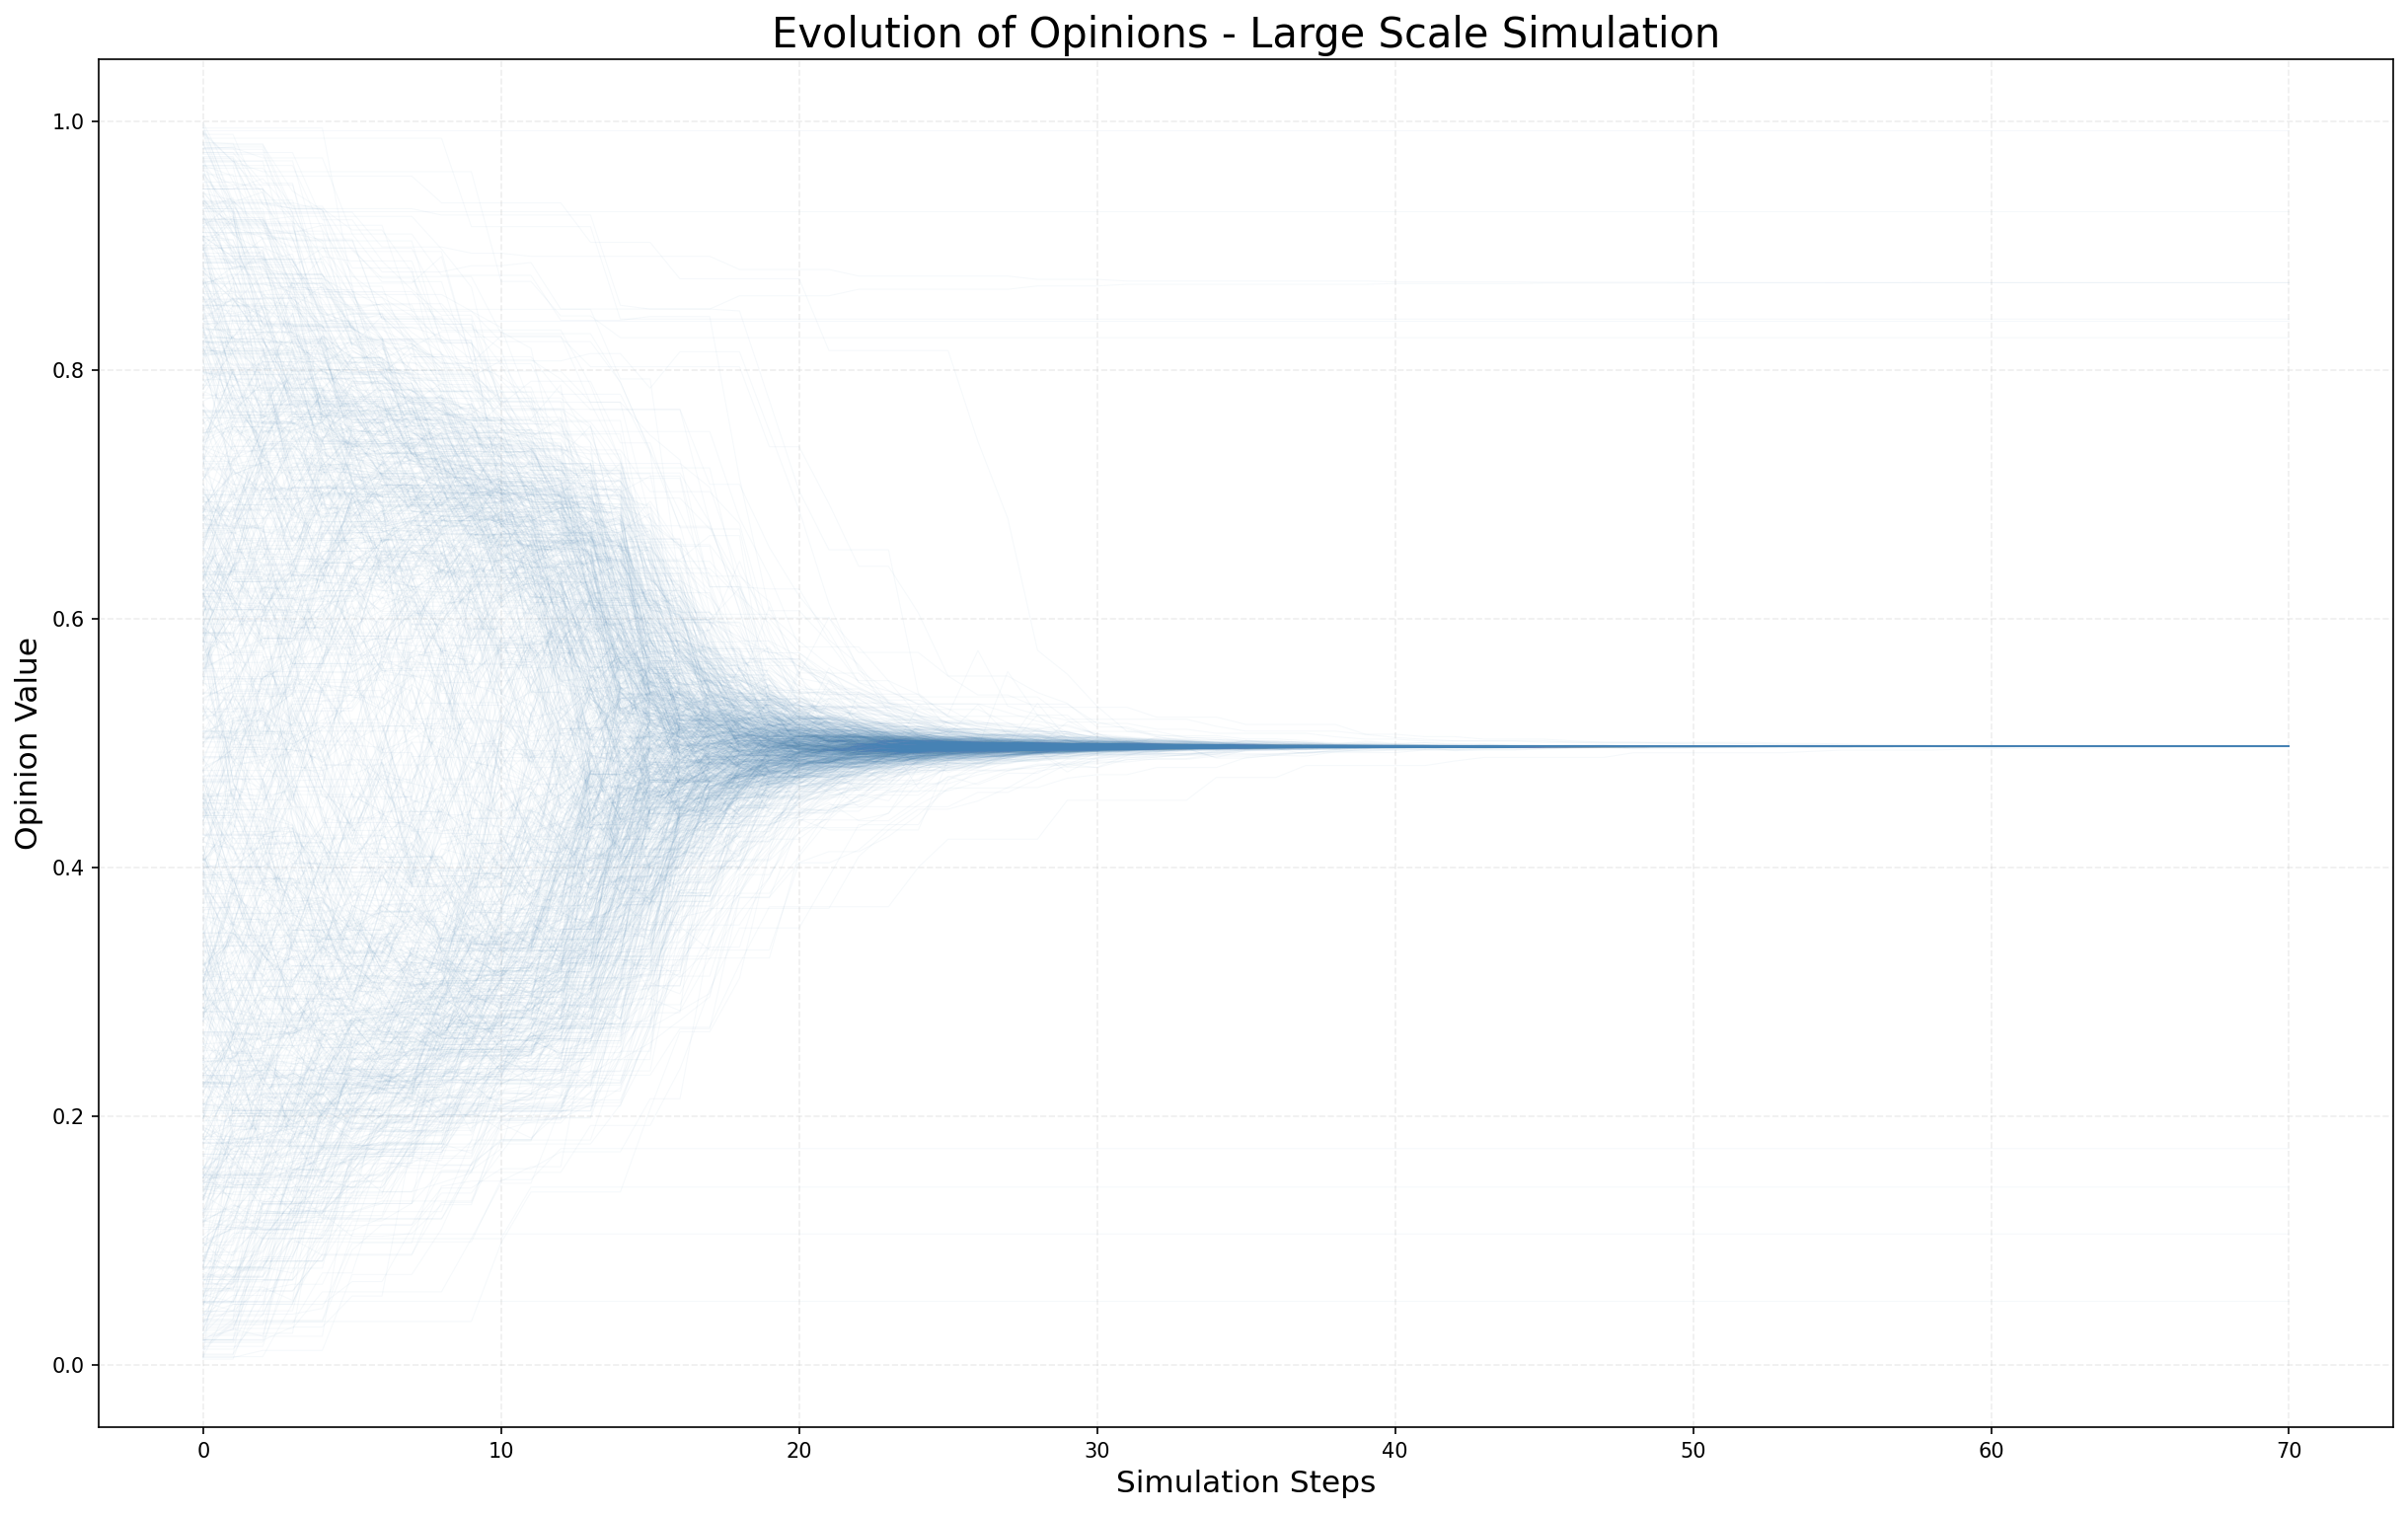
\includegraphics[width=0.33\linewidth]{results/p_0.3_threshold_0.3/opinions_history}
        \caption{Histórico de opiniones Prob. inter 0.3, confianza 0.3: Consenso}
        \label{fig:p_0.3_threshold_0.3}
    \end{figure}
    \FloatBarrier

    \subsection{Prob. inter 0.5, confianza 0.1}
    \begin{figure}[htbp]
        \centering
        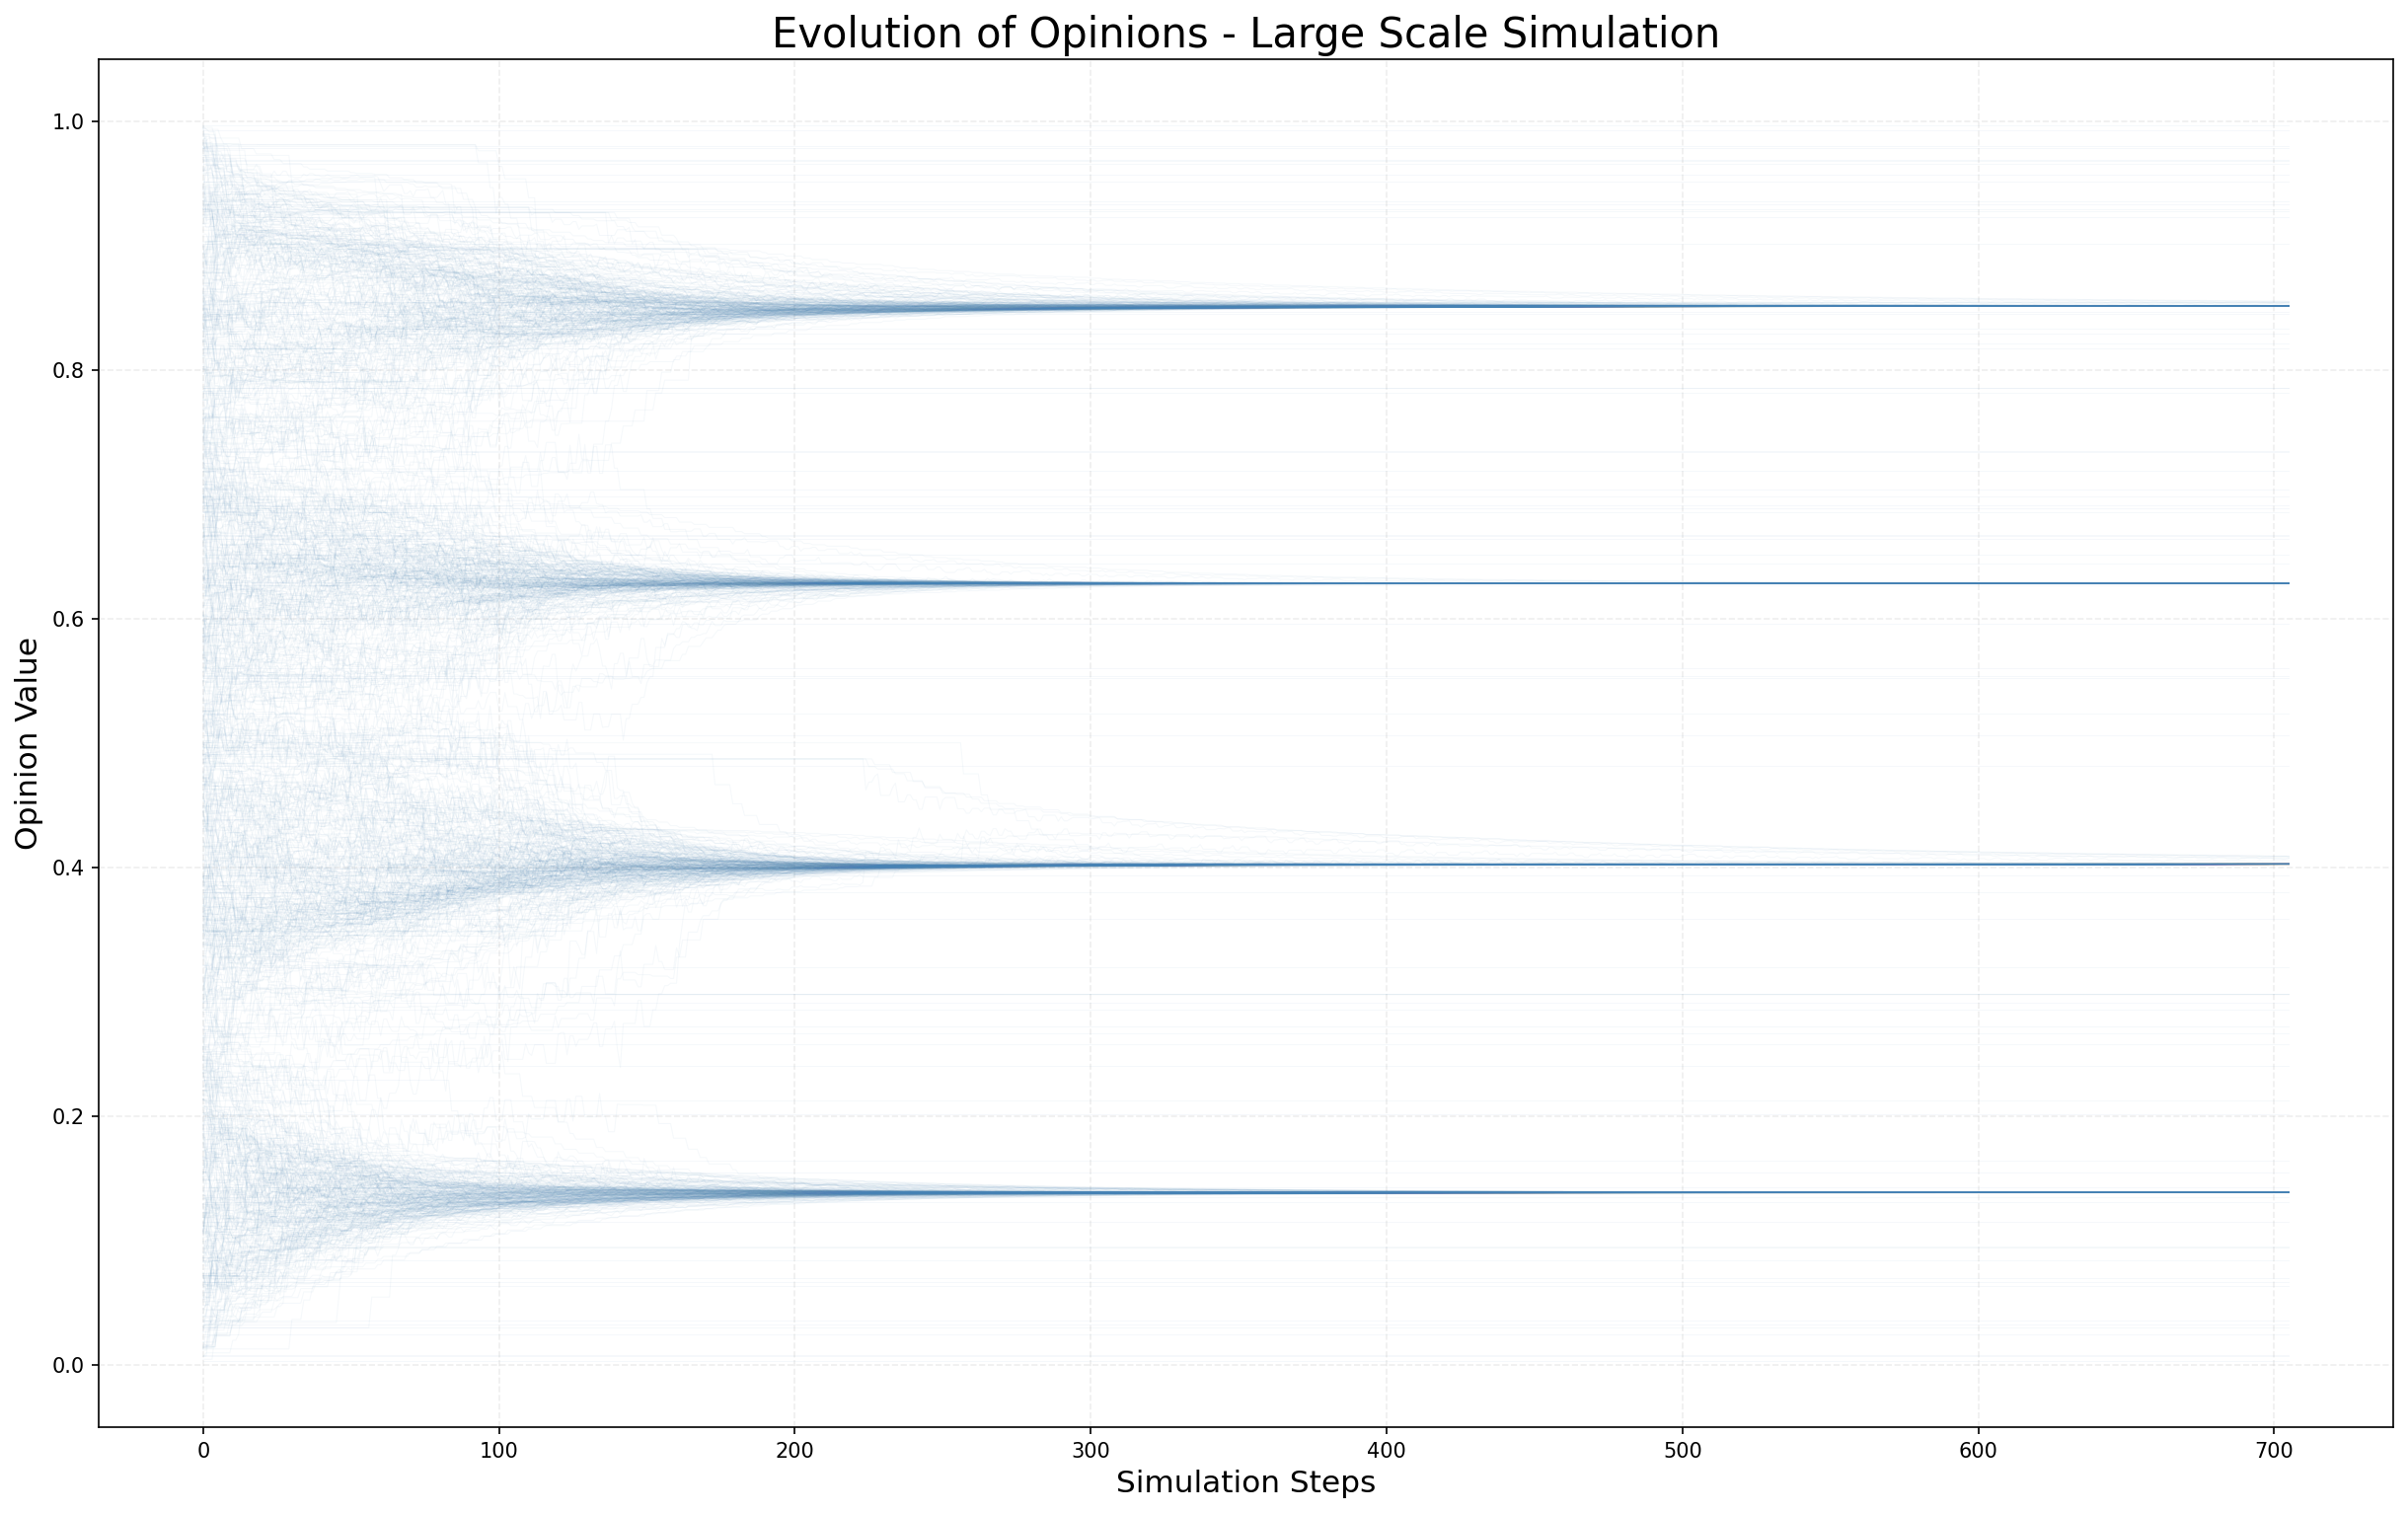
\includegraphics[width=0.33\linewidth]{results/p_0.5_threshold_0.1/opinions_history}
        \caption{Histórico de opiniones Prob. inter 0.5, confianza 0.1 Fragmentación}
        \label{fig:p_0.5_threshold_0.1}
    \end{figure}
    \FloatBarrier

    \subsection{Prob. inter 0.5, confianza 0.15}


    \subsection{Prob. inter 0.5, confianza 0.2}
    \begin{figure}[htbp]
        \centering
        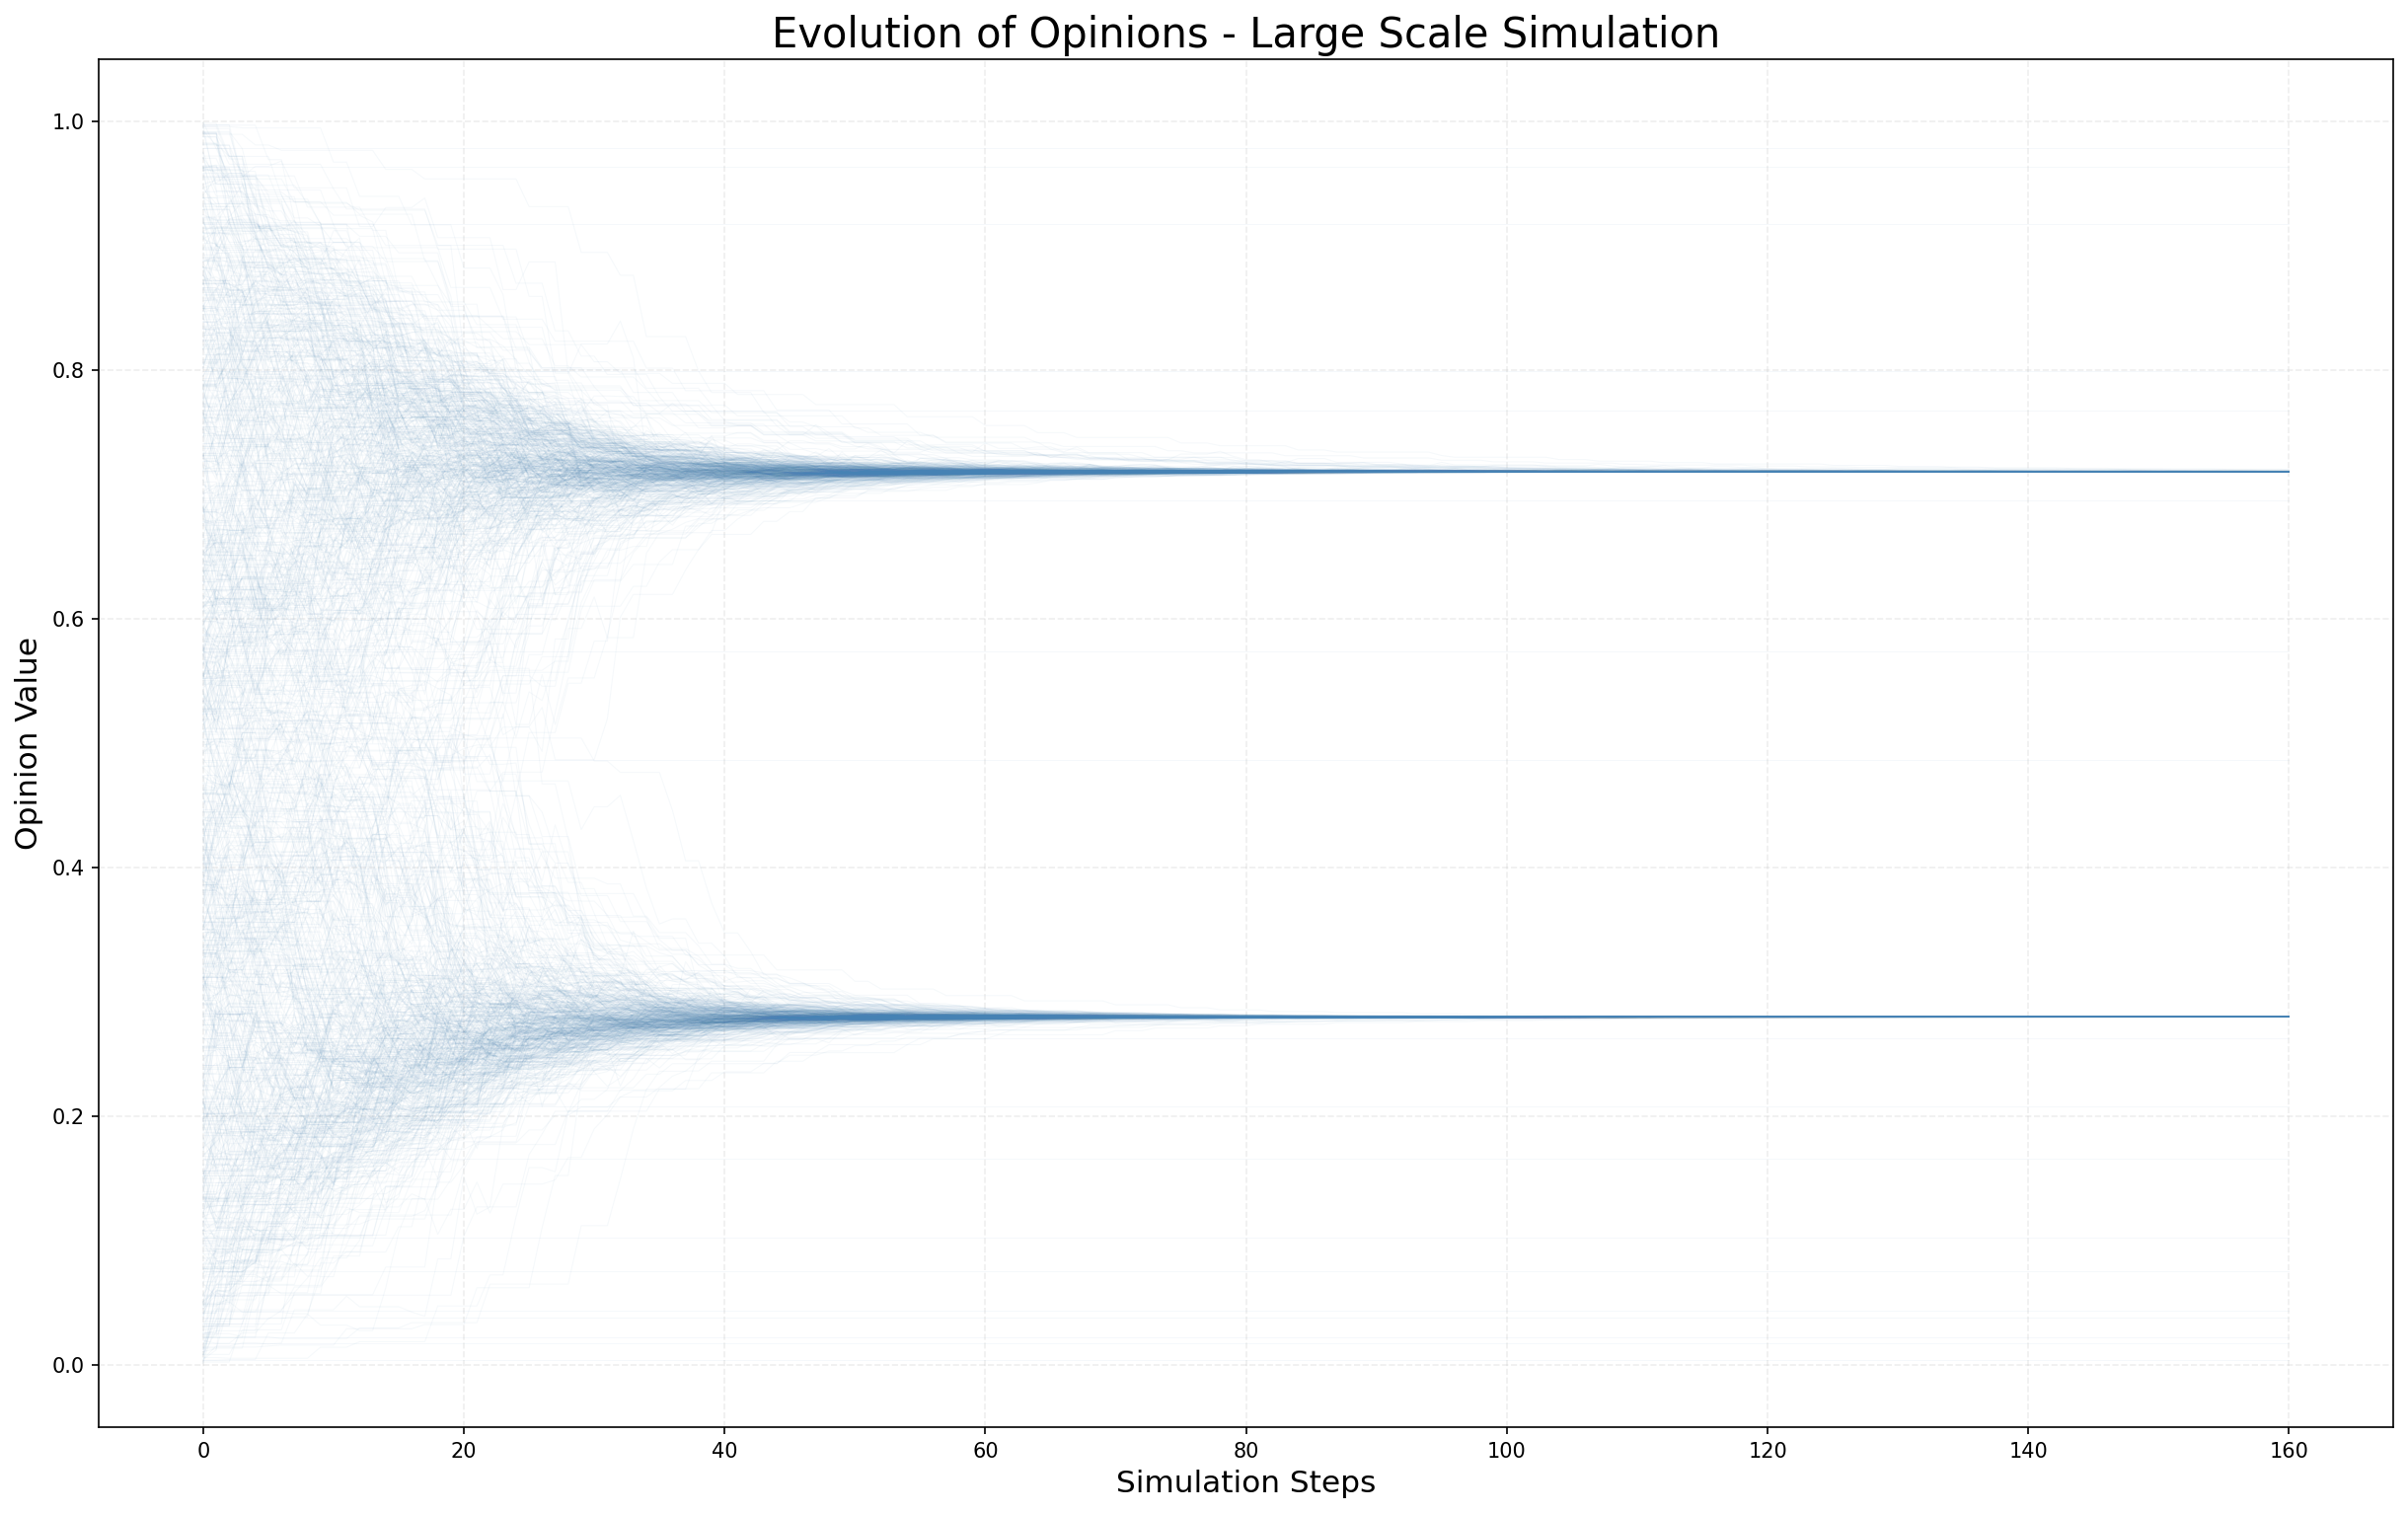
\includegraphics[width=0.33\linewidth]{results/p_0.5_threshold_0.2/opinions_history}
        \caption{Histórico de opiniones Prob. inter 0.5, confianza 0.2: Polarización}
        \label{fig:p_0.5_threshold_0.2}
    \end{figure}
    \FloatBarrier

    \subsection{Prob. inter 0.5, confianza 0.25}
    \begin{figure}[htbp]
        \centering
        \begin{subfigure}[b]{0.48\linewidth}
            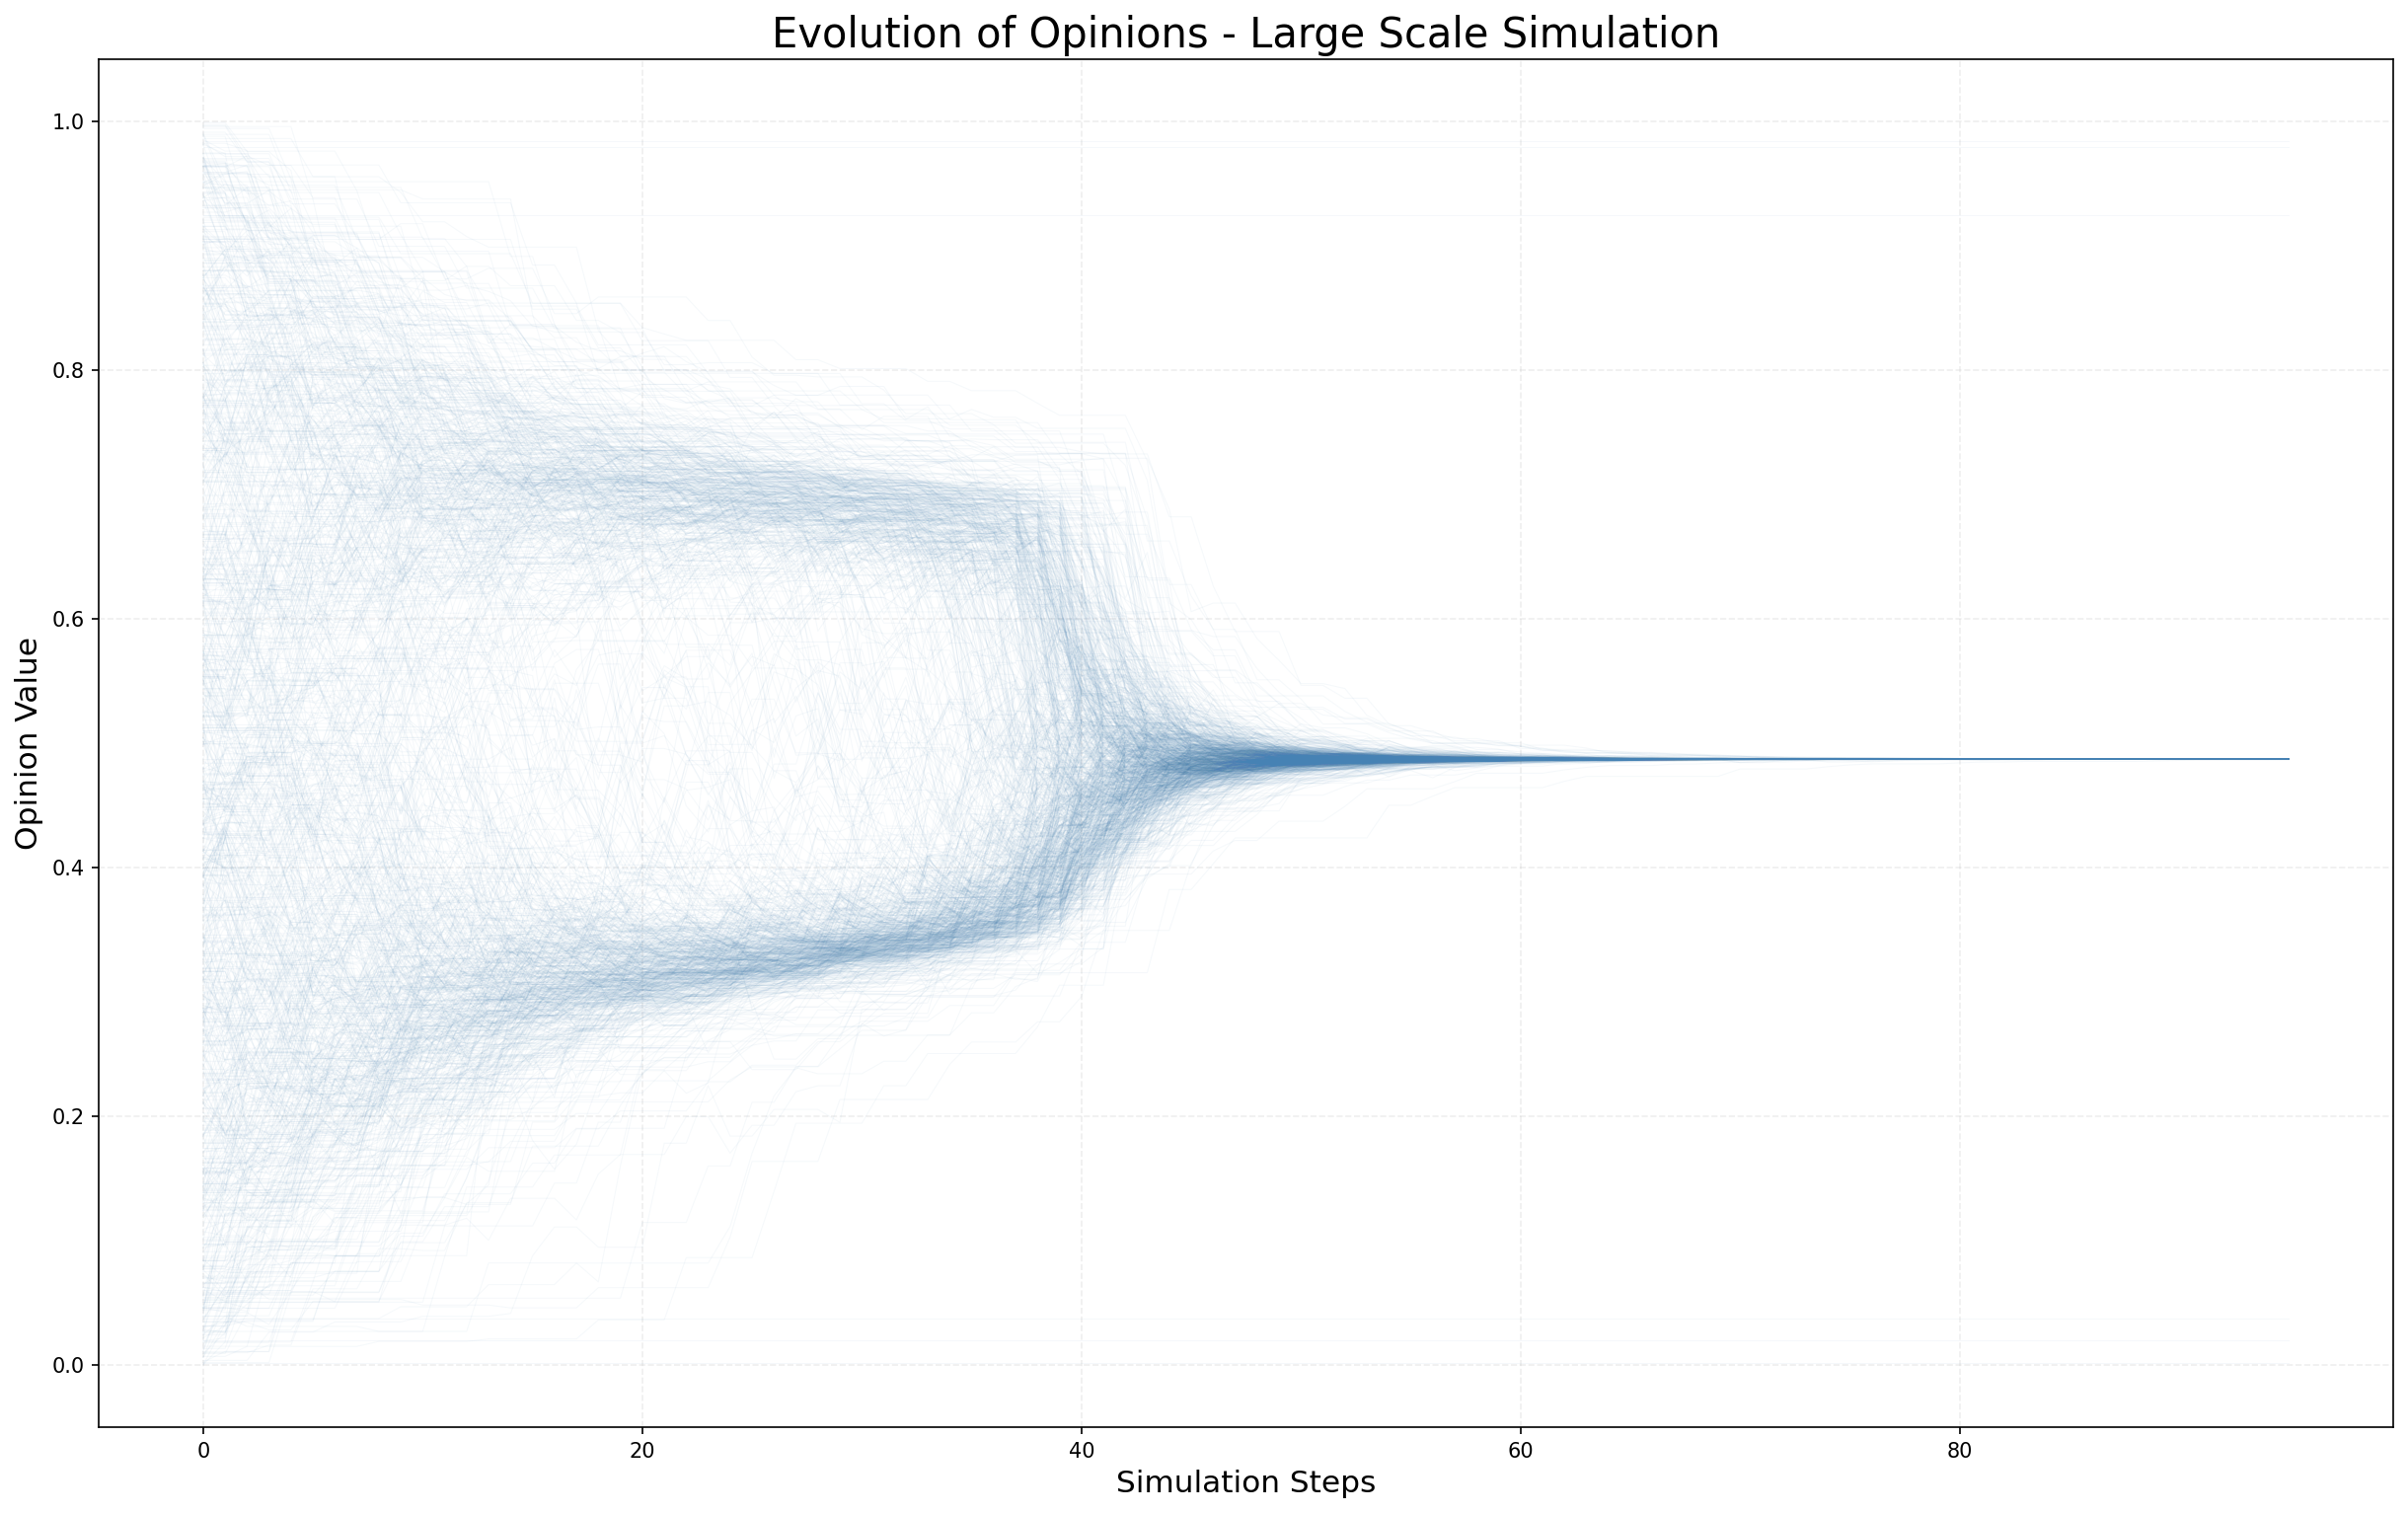
\includegraphics[width=\linewidth]{results/p_0.5_threshold_0.25/opinions_history_1}
            \caption{Consenso}
            \label{fig:p_0.5_threshold_0.25_1}
        \end{subfigure}
        \begin{subfigure}[b]{0.48\linewidth}
            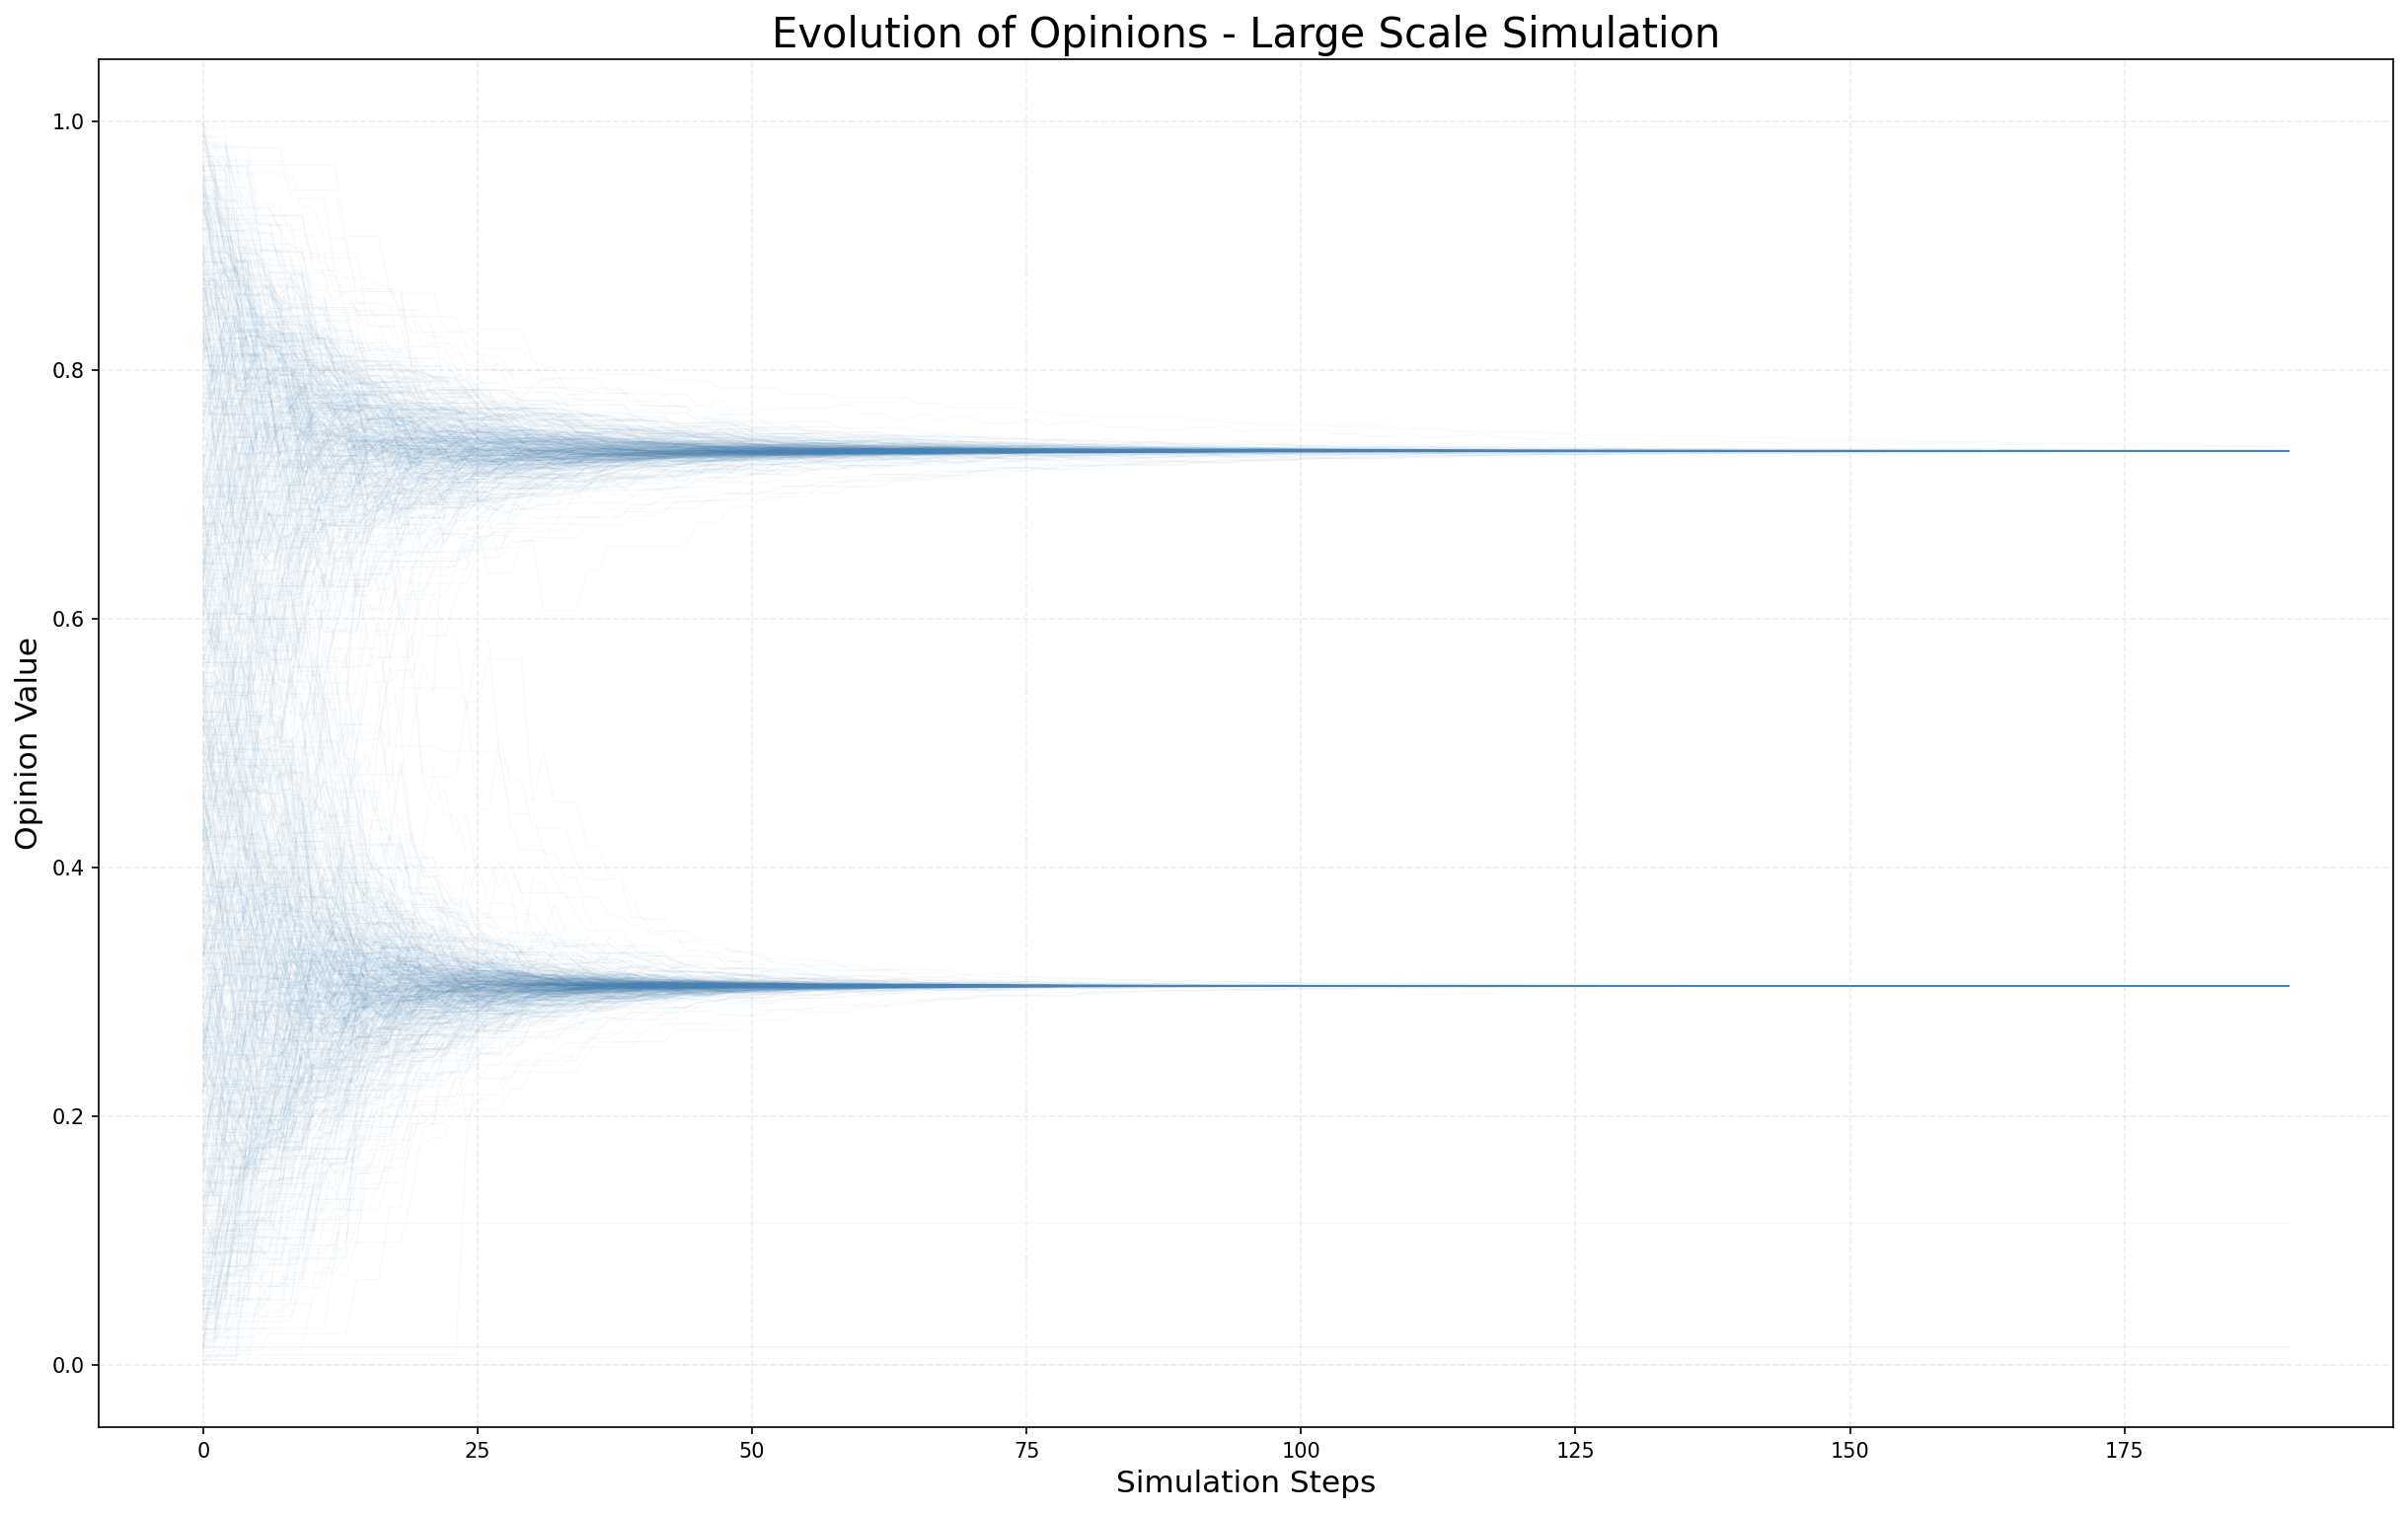
\includegraphics[width=\linewidth]{results/p_0.5_threshold_0.25/opinions_history_2}
            \caption{Fragmentación}
            \label{fig:p_0.5_threshold_0.25_2}
        \end{subfigure}
        \caption{Histórico de opiniones Prob. inter 0.5, confianza 0.25}
        \label{fig:p_0.5_threshold_0.25}
    \end{figure}
    \FloatBarrier


    \subsection{Prob. inter 0.5, confianza 0.3}
    \begin{figure}[htbp]
        \centering
        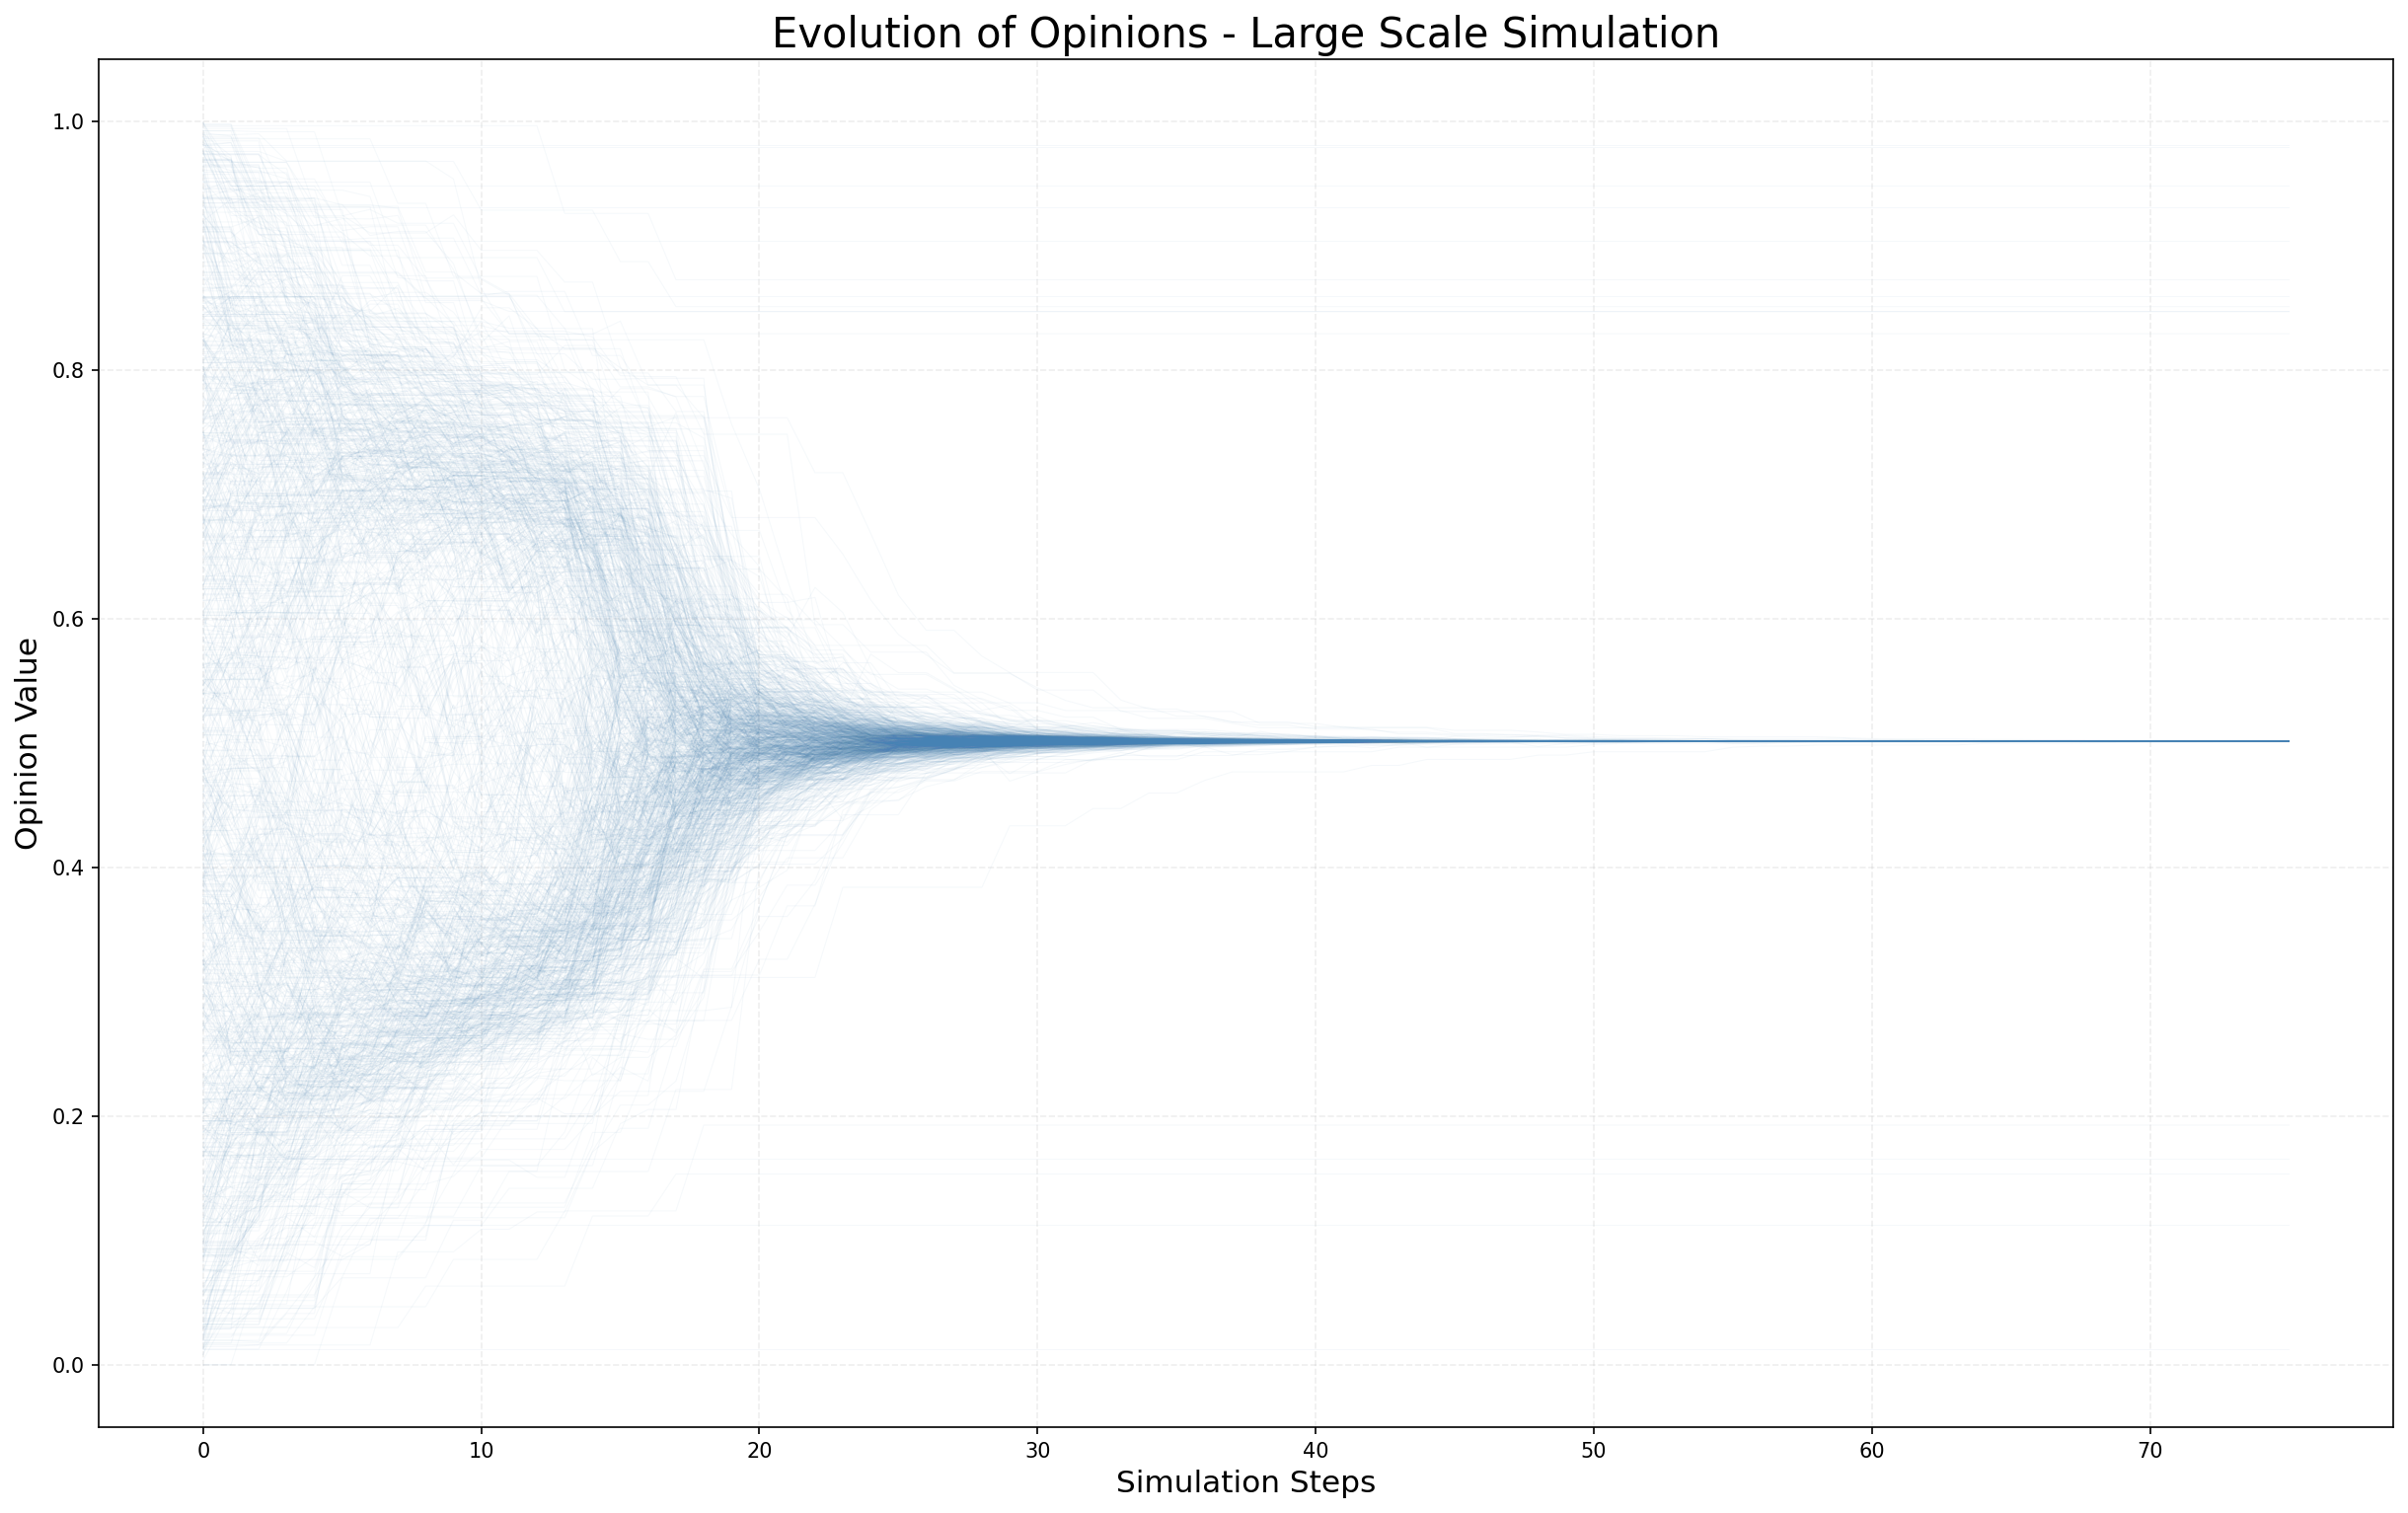
\includegraphics[width=0.33\linewidth]{results/p_0.5_threshold_0.3/opinions_history}
        \caption{Histórico de opiniones Prob. inter 0.5, confianza 0.3: Consenso}
        \label{fig:p_0.5_threshold_0.3}
    \end{figure}
    \FloatBarrier


    \subsection{Prob. inter 0.7, confianza 0.1}


    \subsection{Prob. inter 0.7, confianza 0.15}
    \begin{figure}[htbp]
        \centering
        \begin{subfigure}[b]{0.48\linewidth}
            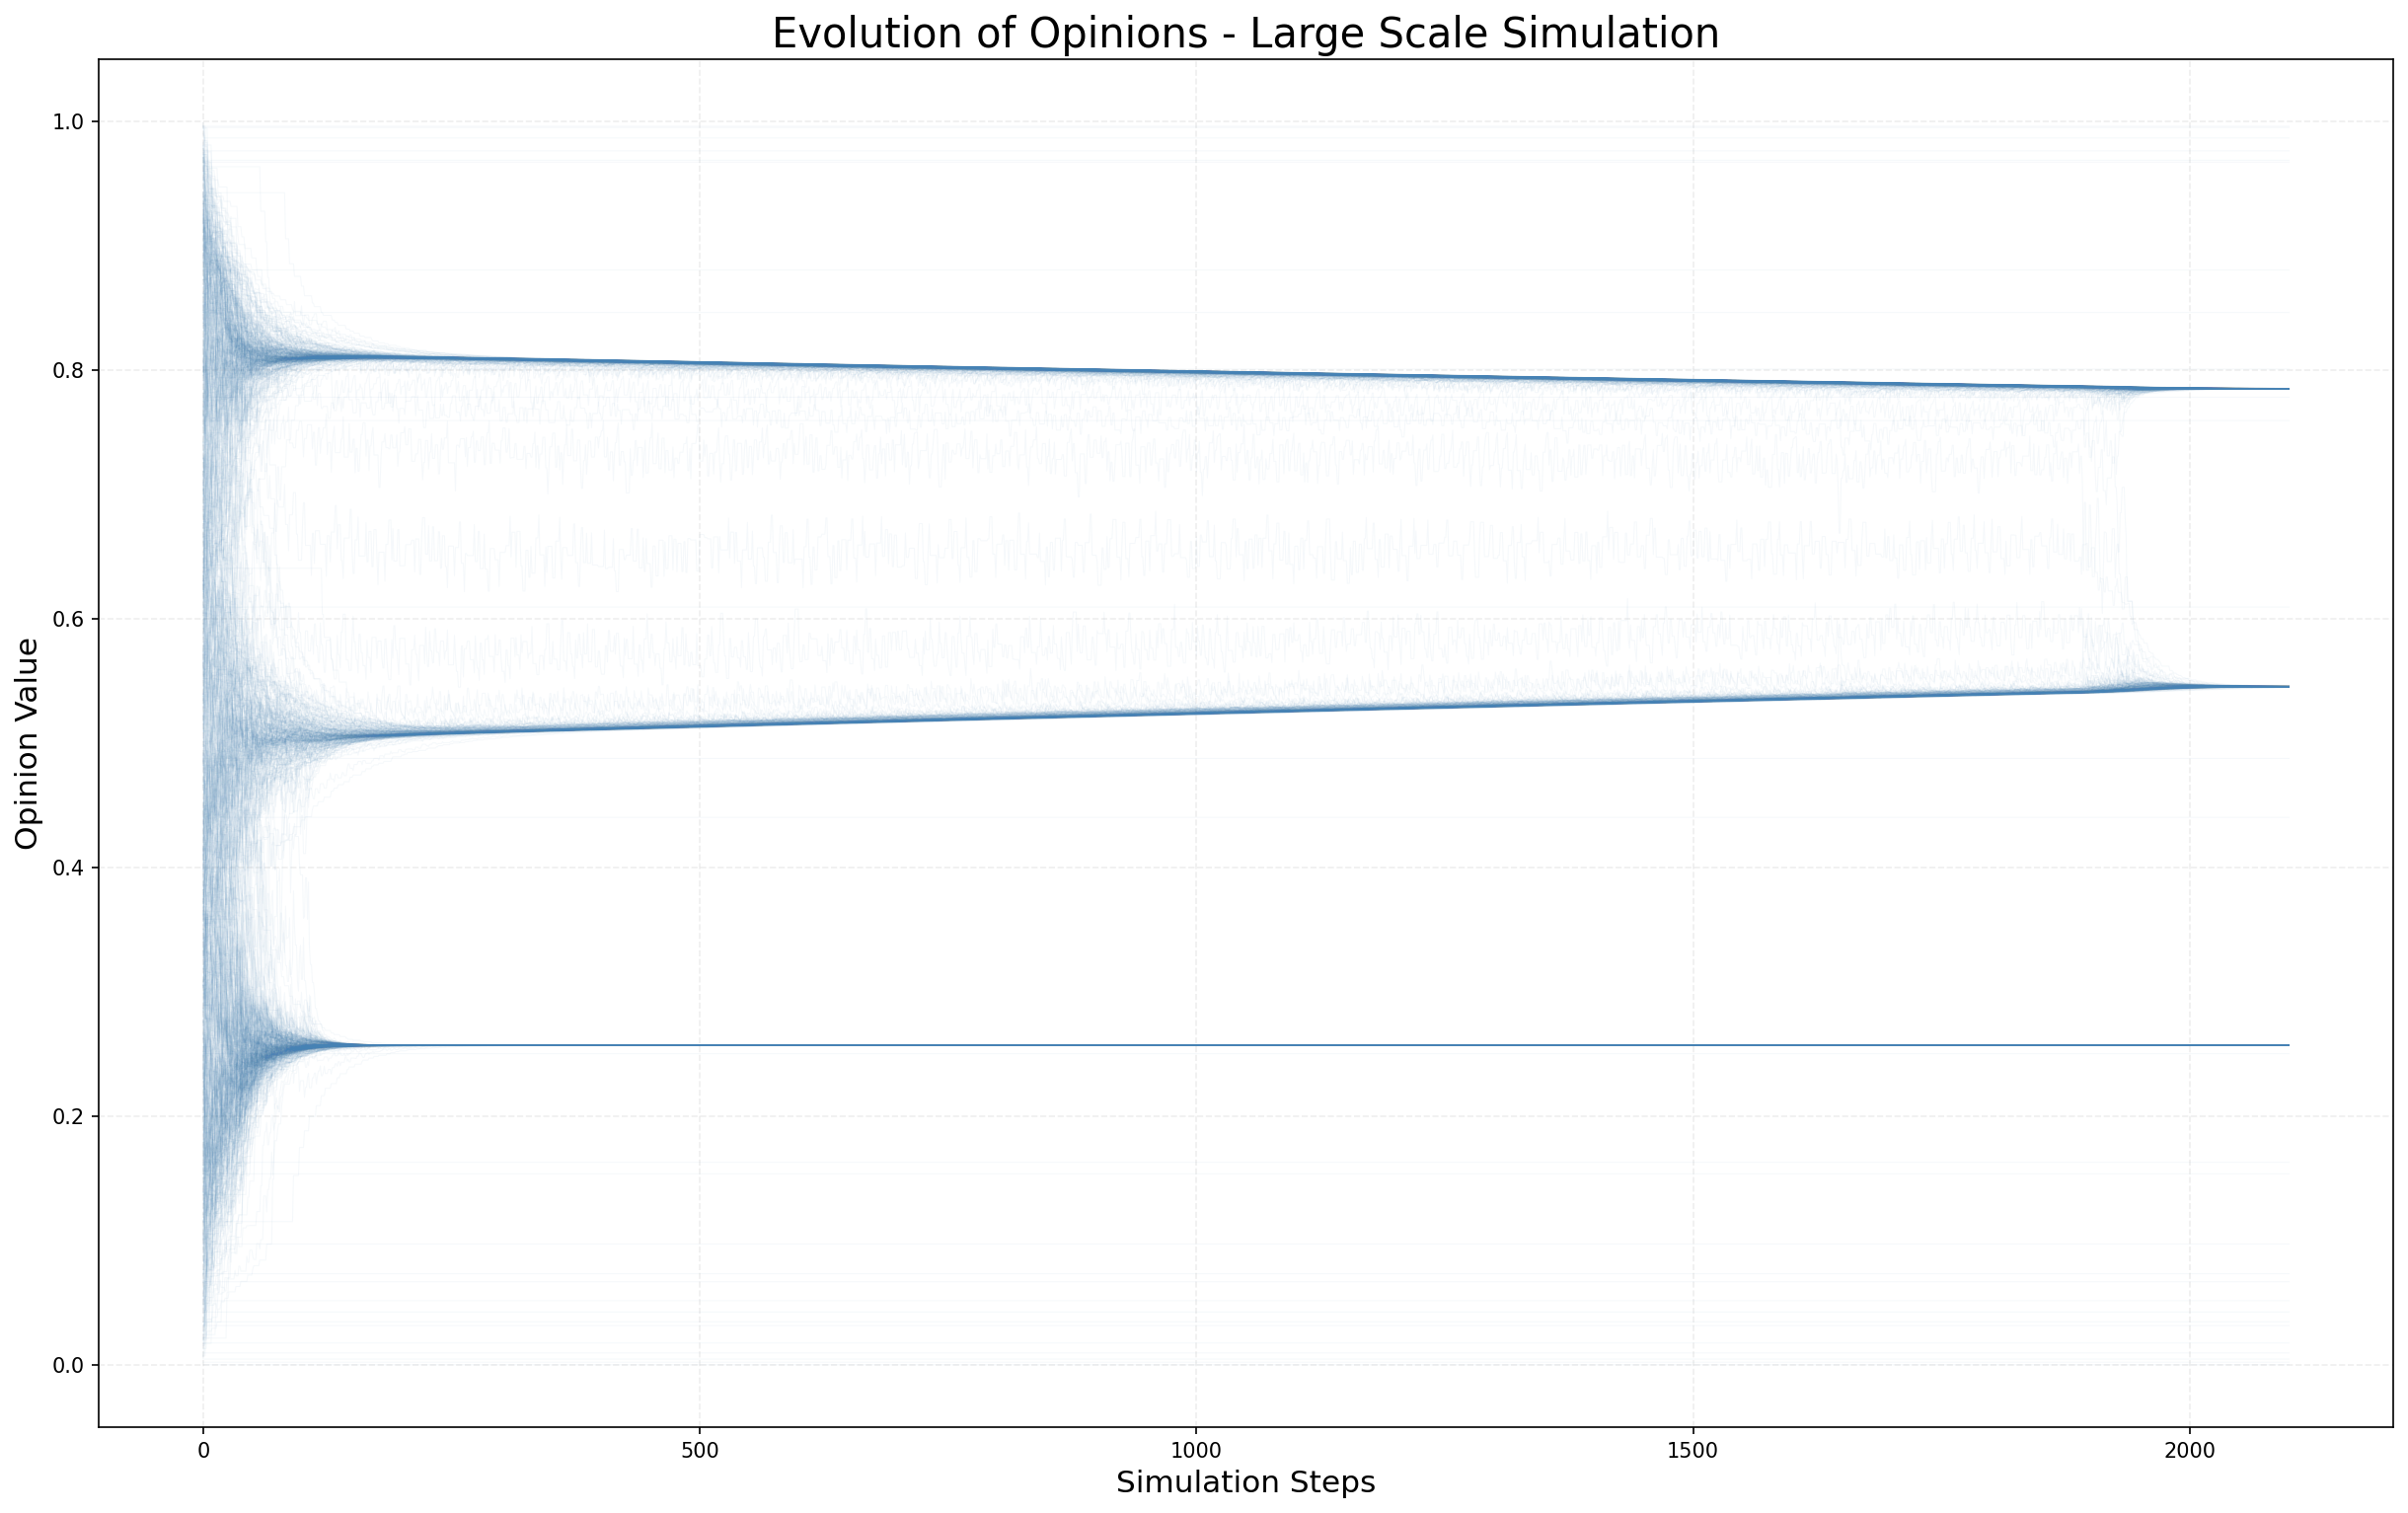
\includegraphics[width=\linewidth]{results/p_0.7_threshold_0.15/opinions_history_1}
            \caption{Fragmentación}
            \label{fig:p_0.7_threshold_0.15_1}
        \end{subfigure}
        \begin{subfigure}[b]{0.48\linewidth}
            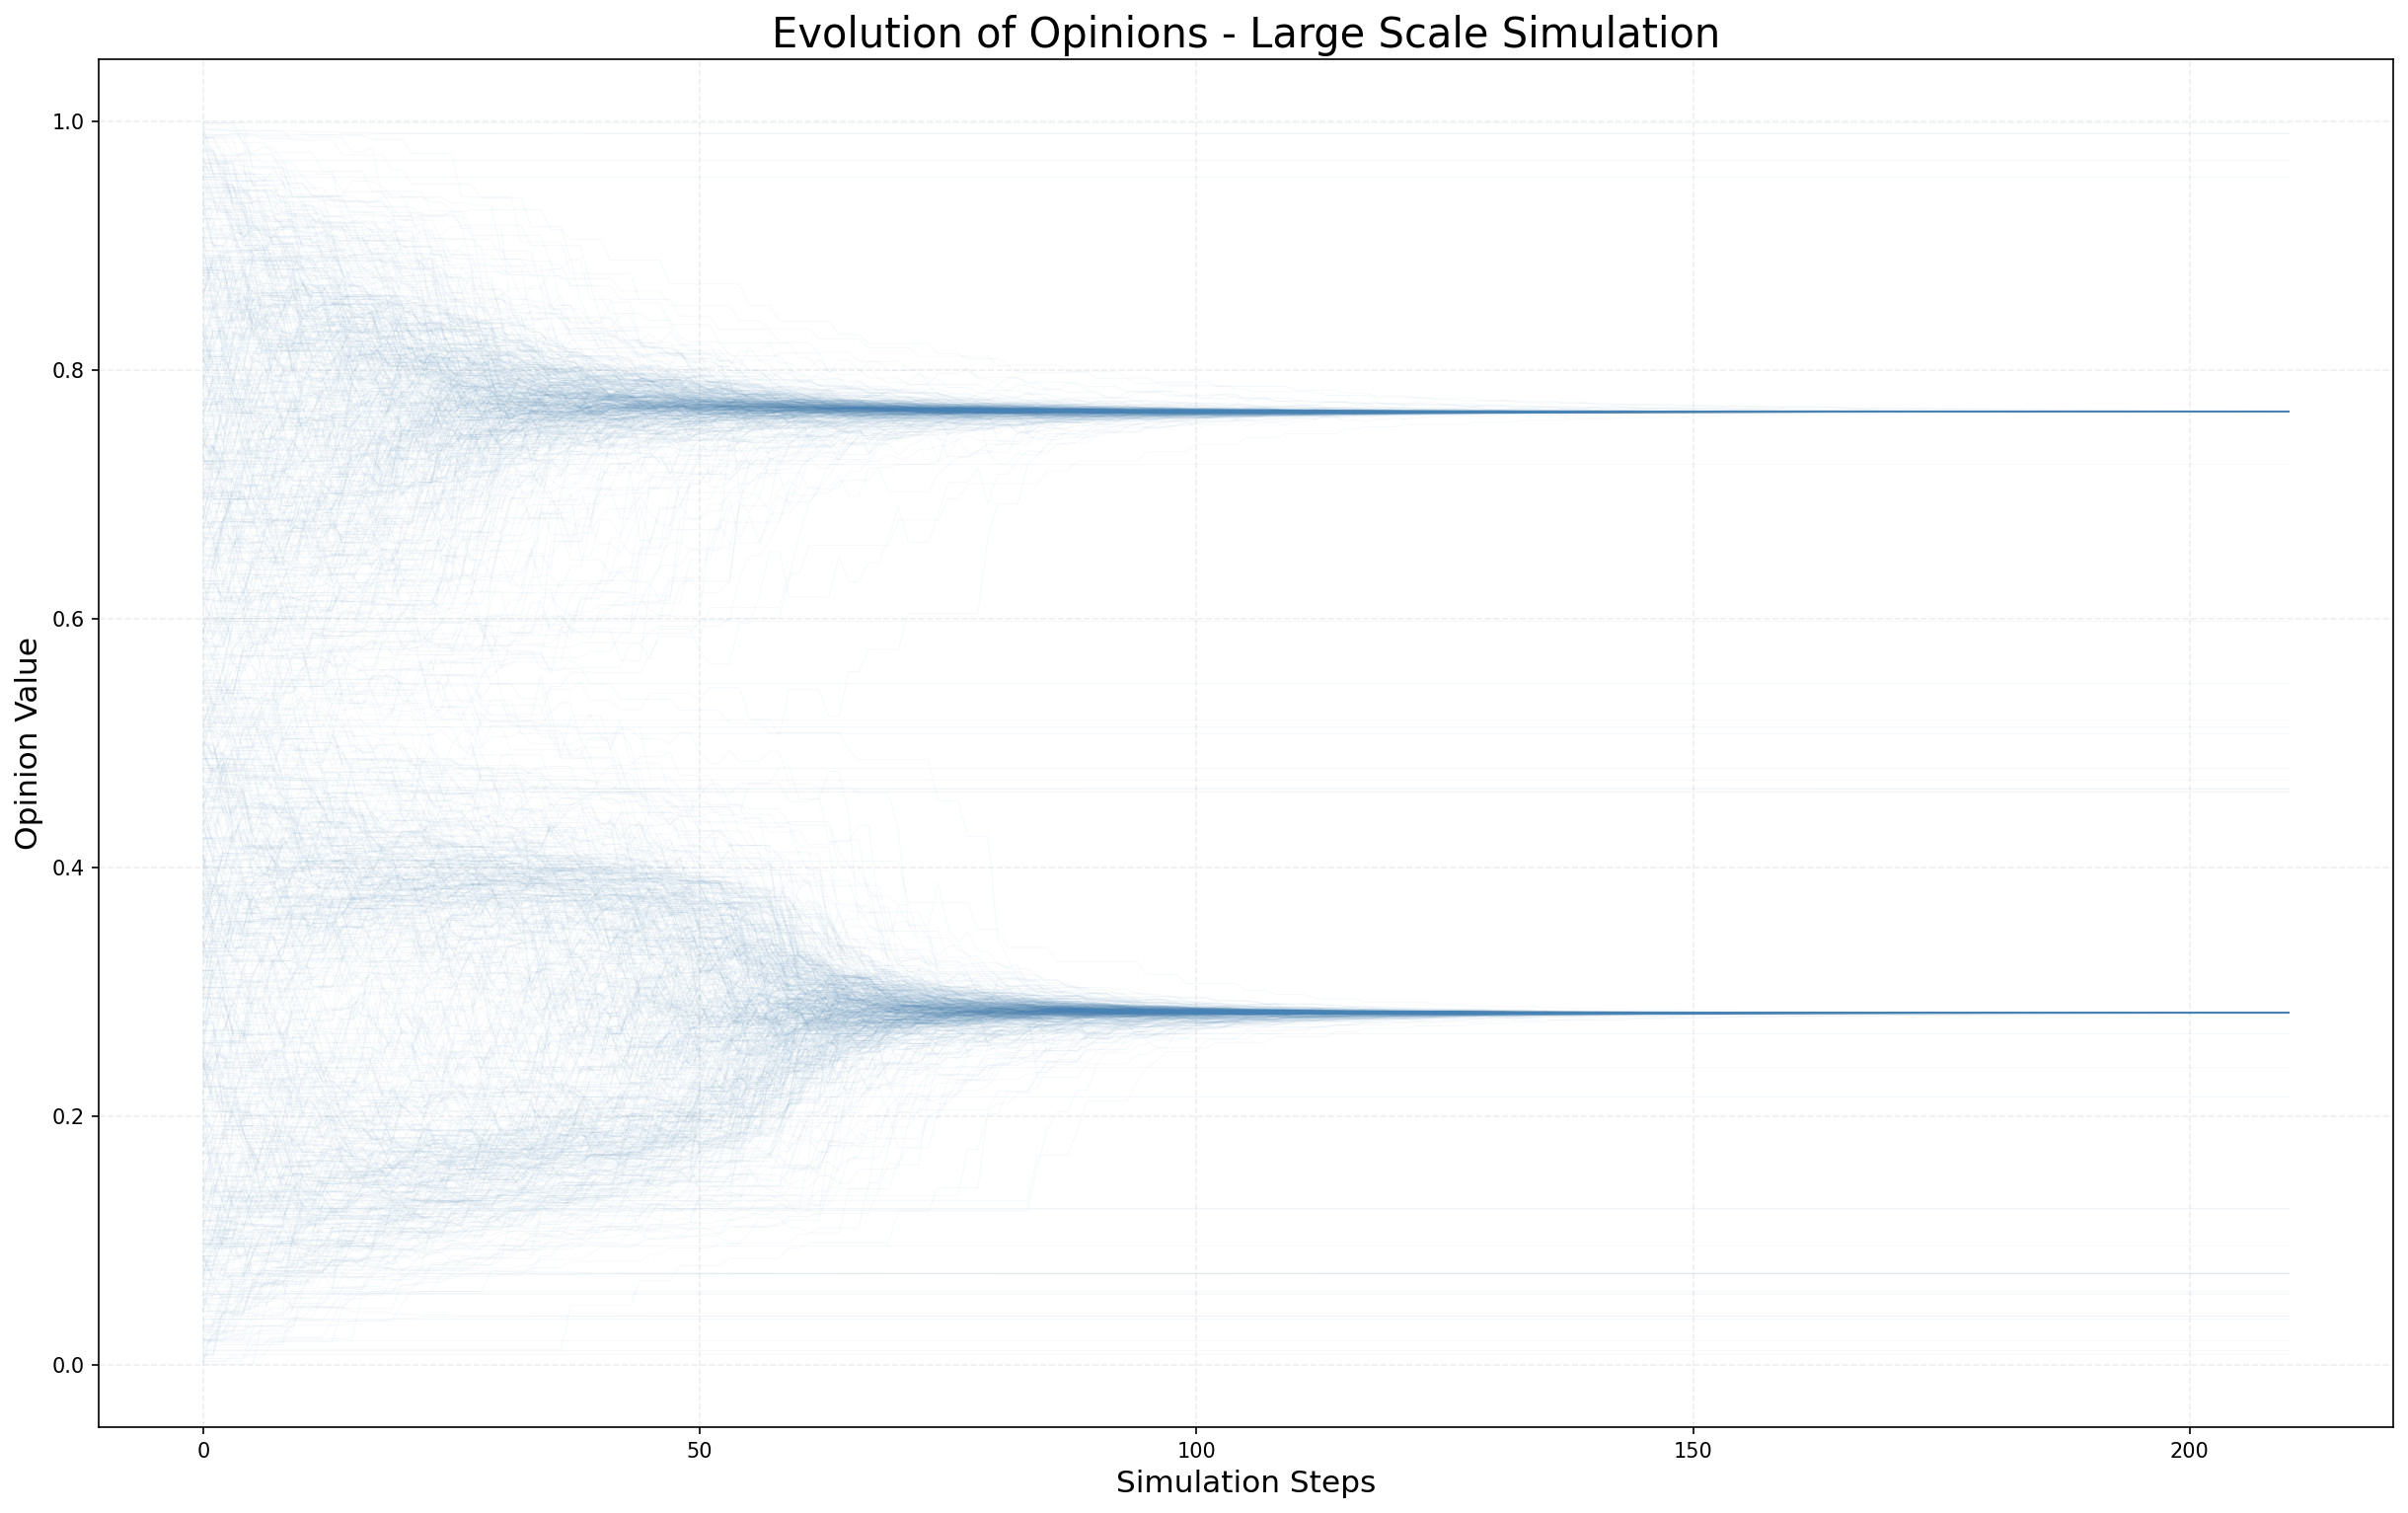
\includegraphics[width=\linewidth]{results/p_0.7_threshold_0.15/opinions_history_2}
            \caption{Polarización}
            \label{fig:p_0.7_threshold_0.15_2}
        \end{subfigure}
        \caption{Histórico de opiniones Prob. inter 0.7, confianza 0.15}
        \label{fig:p_0.7_threshold_0.15}
    \end{figure}
    \FloatBarrier

    \subsection{Prob. inter 0.7, confianza 0.2}

    \subsection{Prob. inter 0.7, confianza 0.25}
    \begin{figure}[htbp]
        \centering
        \begin{subfigure}[b]{0.48\linewidth}
            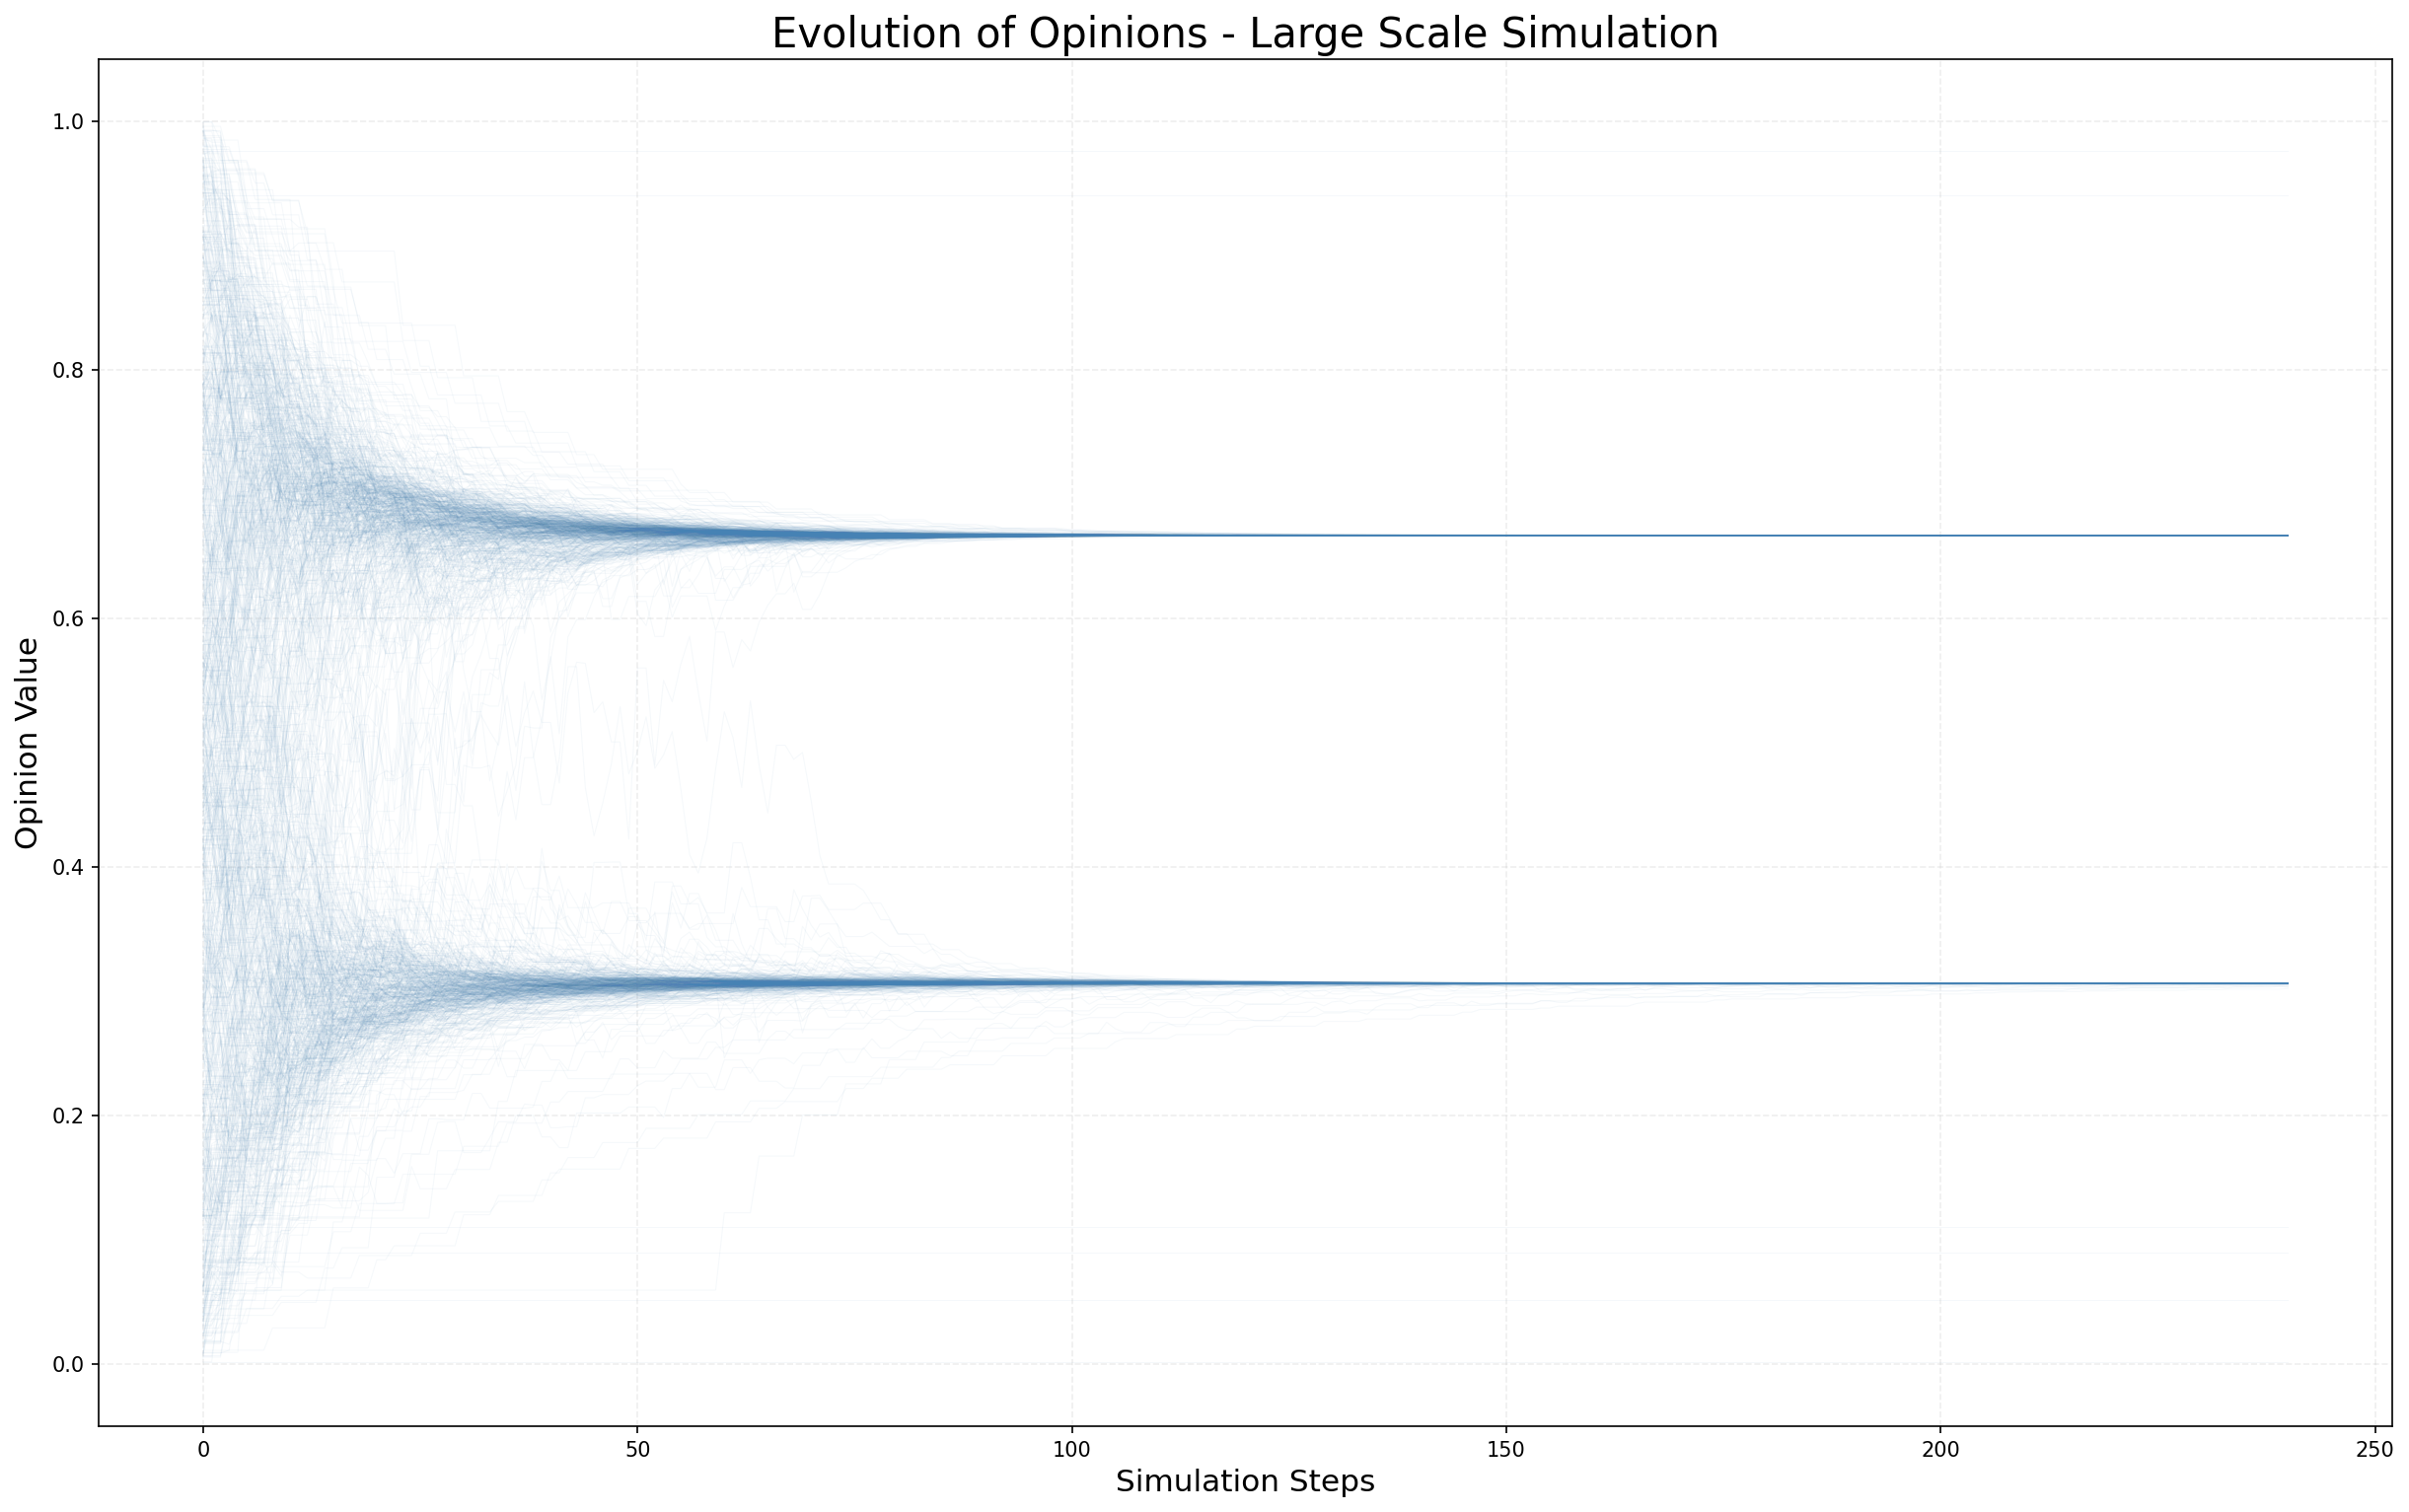
\includegraphics[width=\linewidth]{results/p_0.7_threshold_0.25/opinions_history_1}
            \caption{Polarización}
            \label{fig:p_0.7_threshold_0.25_1}
        \end{subfigure}
        \begin{subfigure}[b]{0.48\linewidth}
            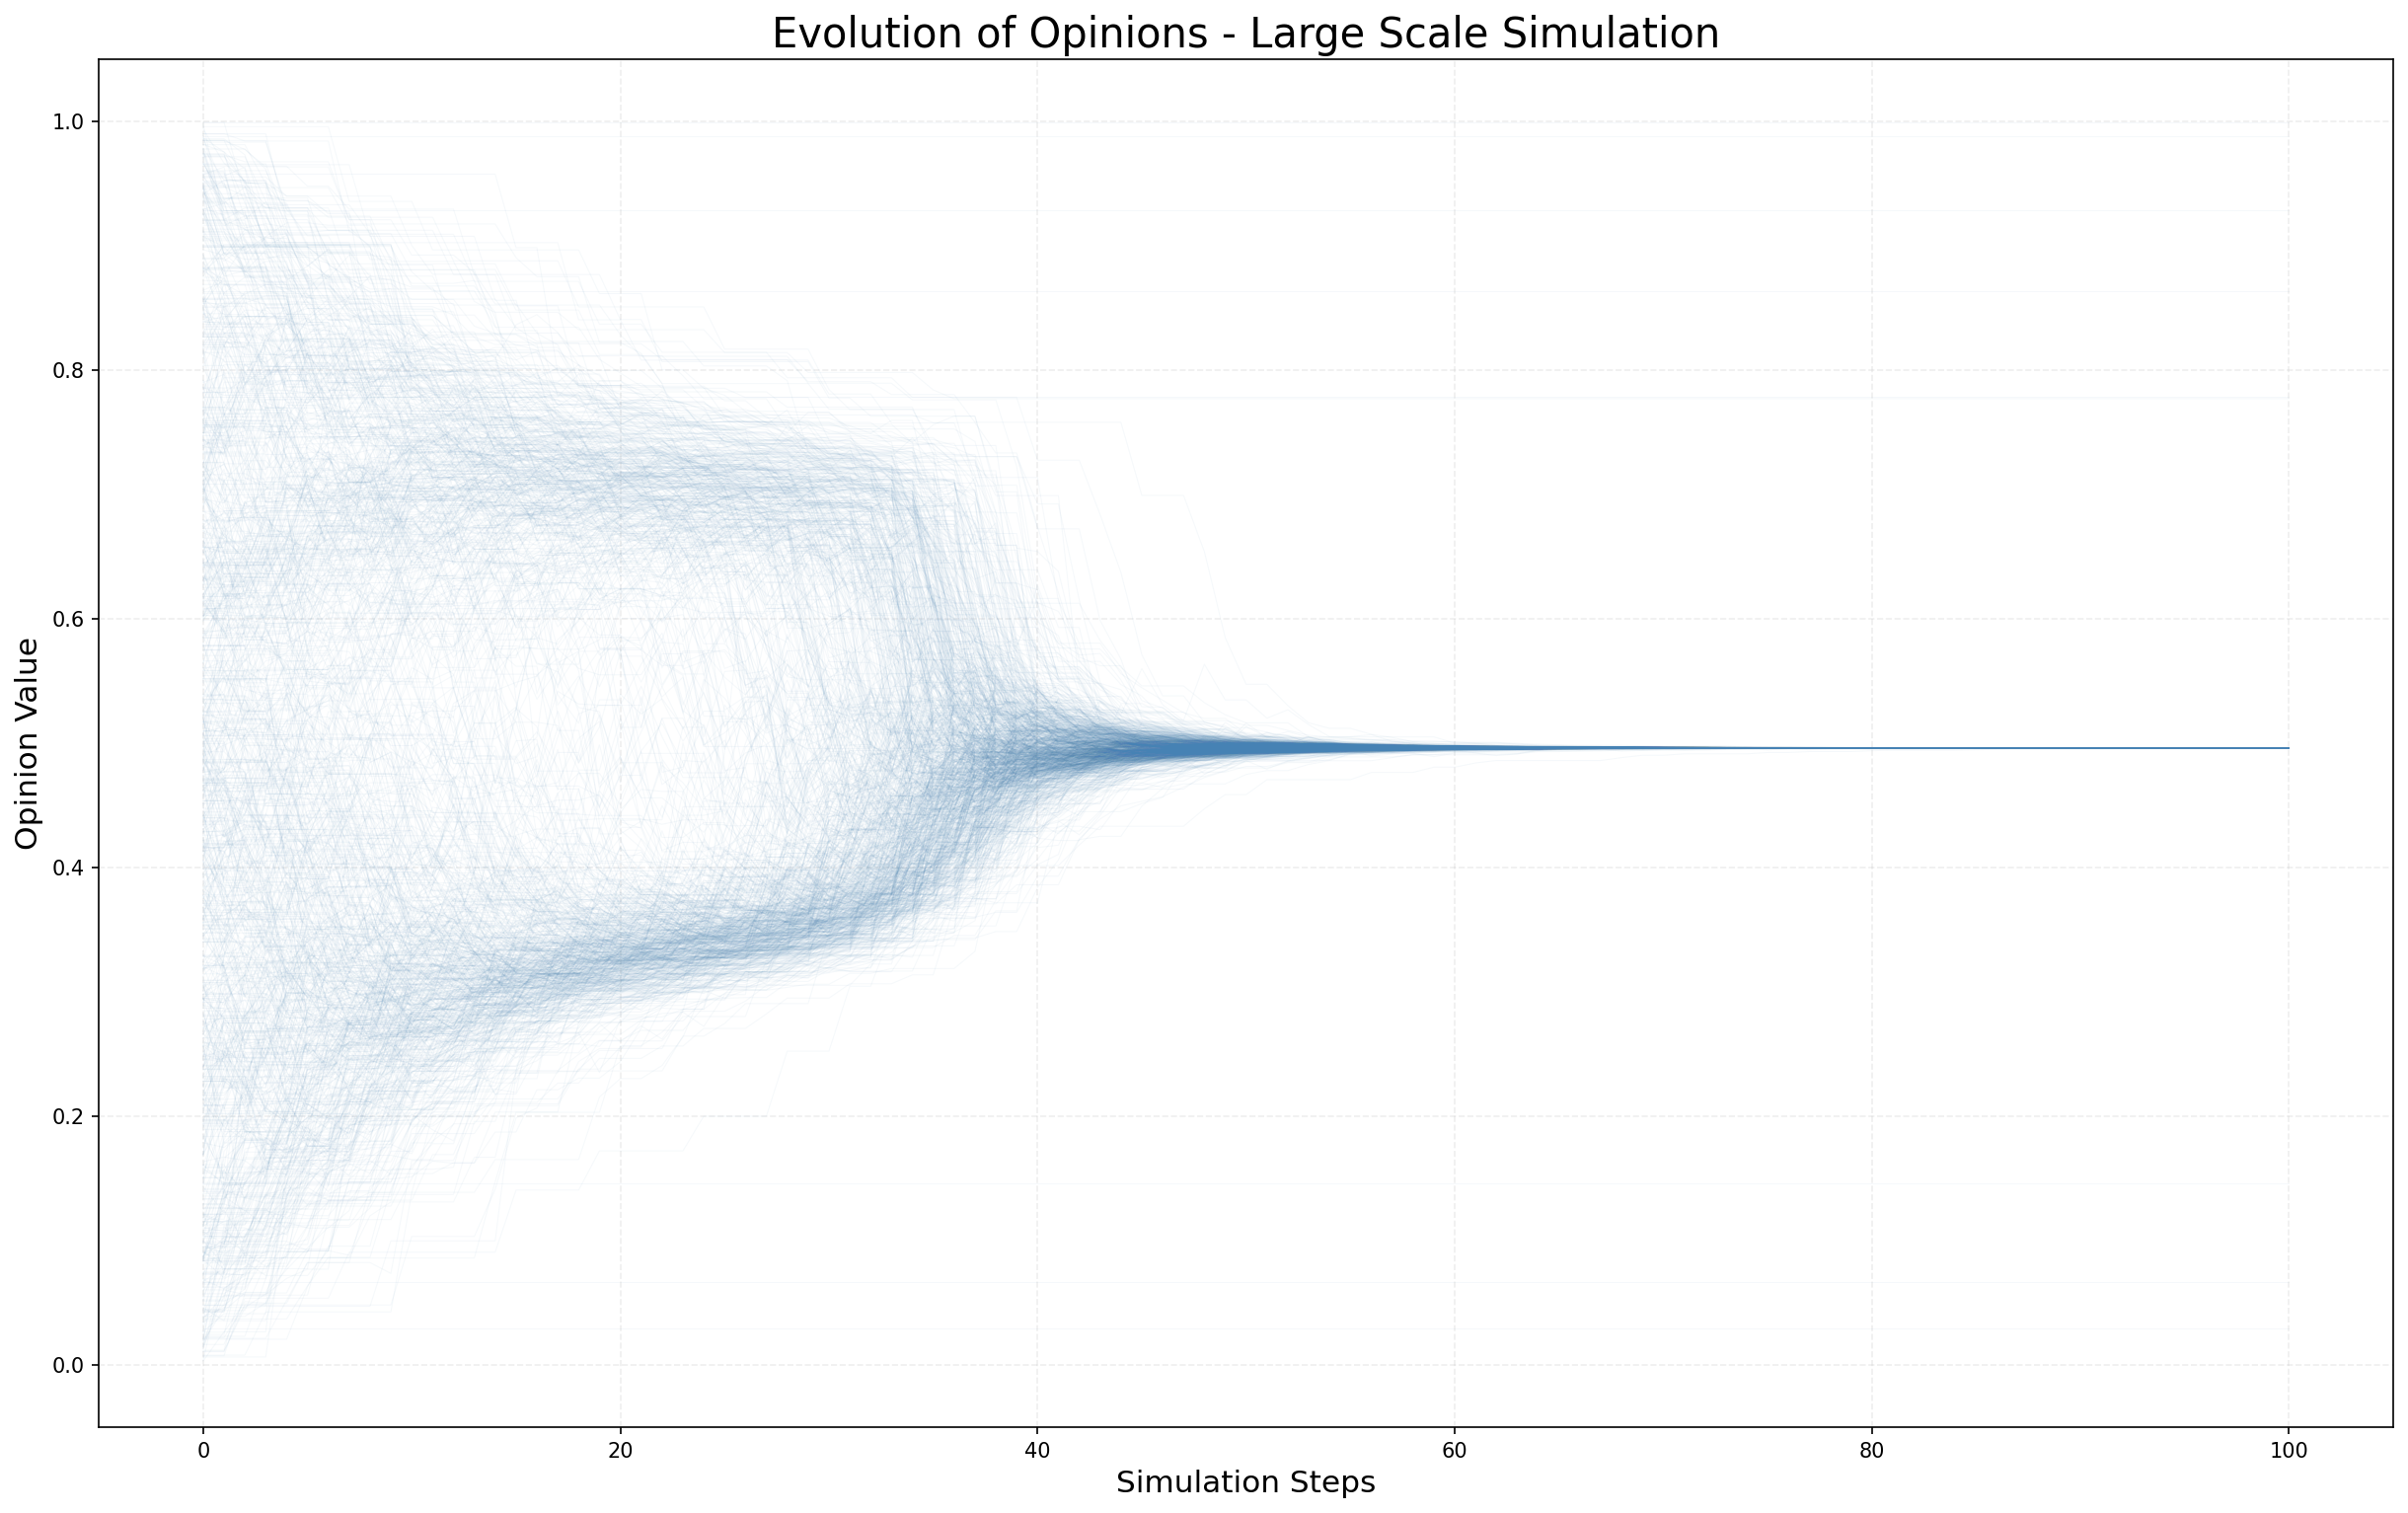
\includegraphics[width=\linewidth]{results/p_0.7_threshold_0.25/opinions_history_2}
            \caption{Consenso}
            \label{fig:p_0.7_threshold_0.25_2}
        \end{subfigure}
        \caption{Histórico de opiniones Prob. inter 0.7, confianza 0.25}
        \label{fig:p_0.7_threshold_0.25}
    \end{figure}
    \FloatBarrier

    \subsection{Prob. inter 0.7, confianza 0.3}

    \subsection{Prob. inter 0.9, confianza 0.10}


    \subsection{Prob. inter 0.9, confianza 0.15}

    \subsection{Prob. inter 0.9, confianza 0.2}

    \subsection{Prob. inter 0.9, confianza 0.25}
    \begin{figure}[htbp]
        \centering
        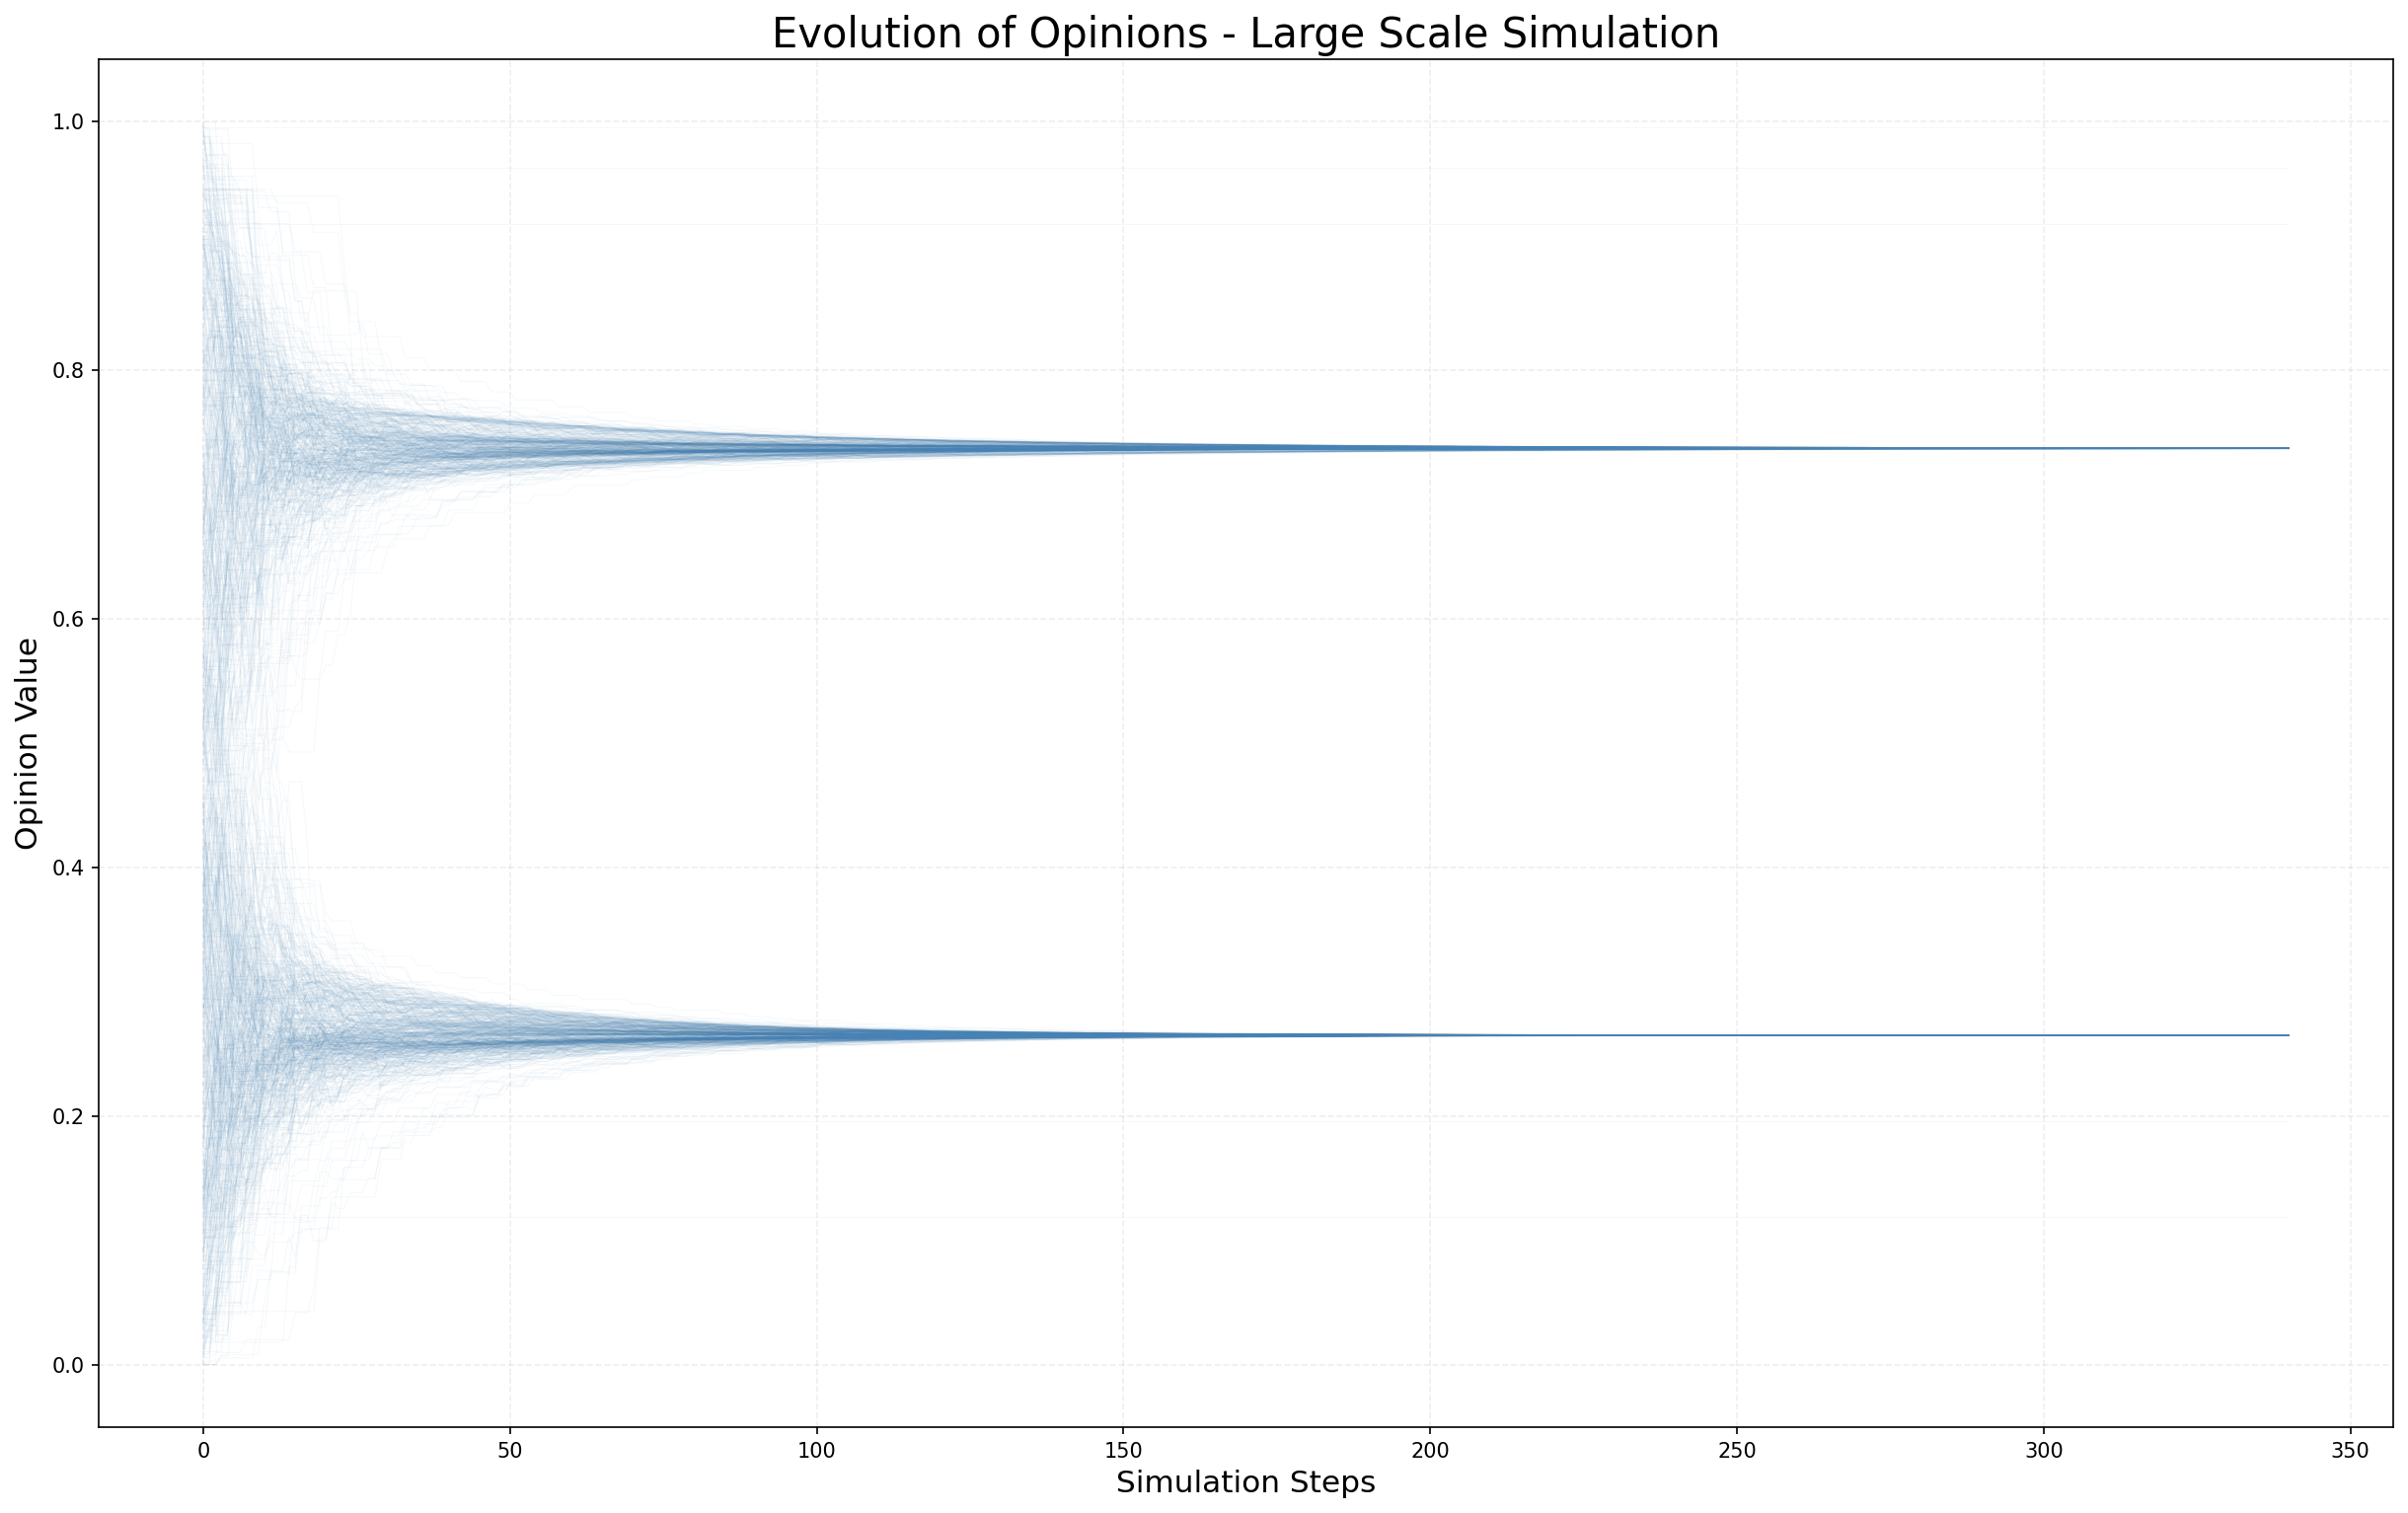
\includegraphics[width=0.33\linewidth]{results/p_0.9_threshold_0.25/opinions_history}
        \caption{Histórico de opiniones Prob. inter 0.9, confianza 0.25: Polarización}
        \label{fig:p_0.9_threshold_0.25}
    \end{figure}
    \FloatBarrier


    \subsection{Prob. inter 0.9, confianza 0.3}
    \begin{figure}[htbp]
        \centering
        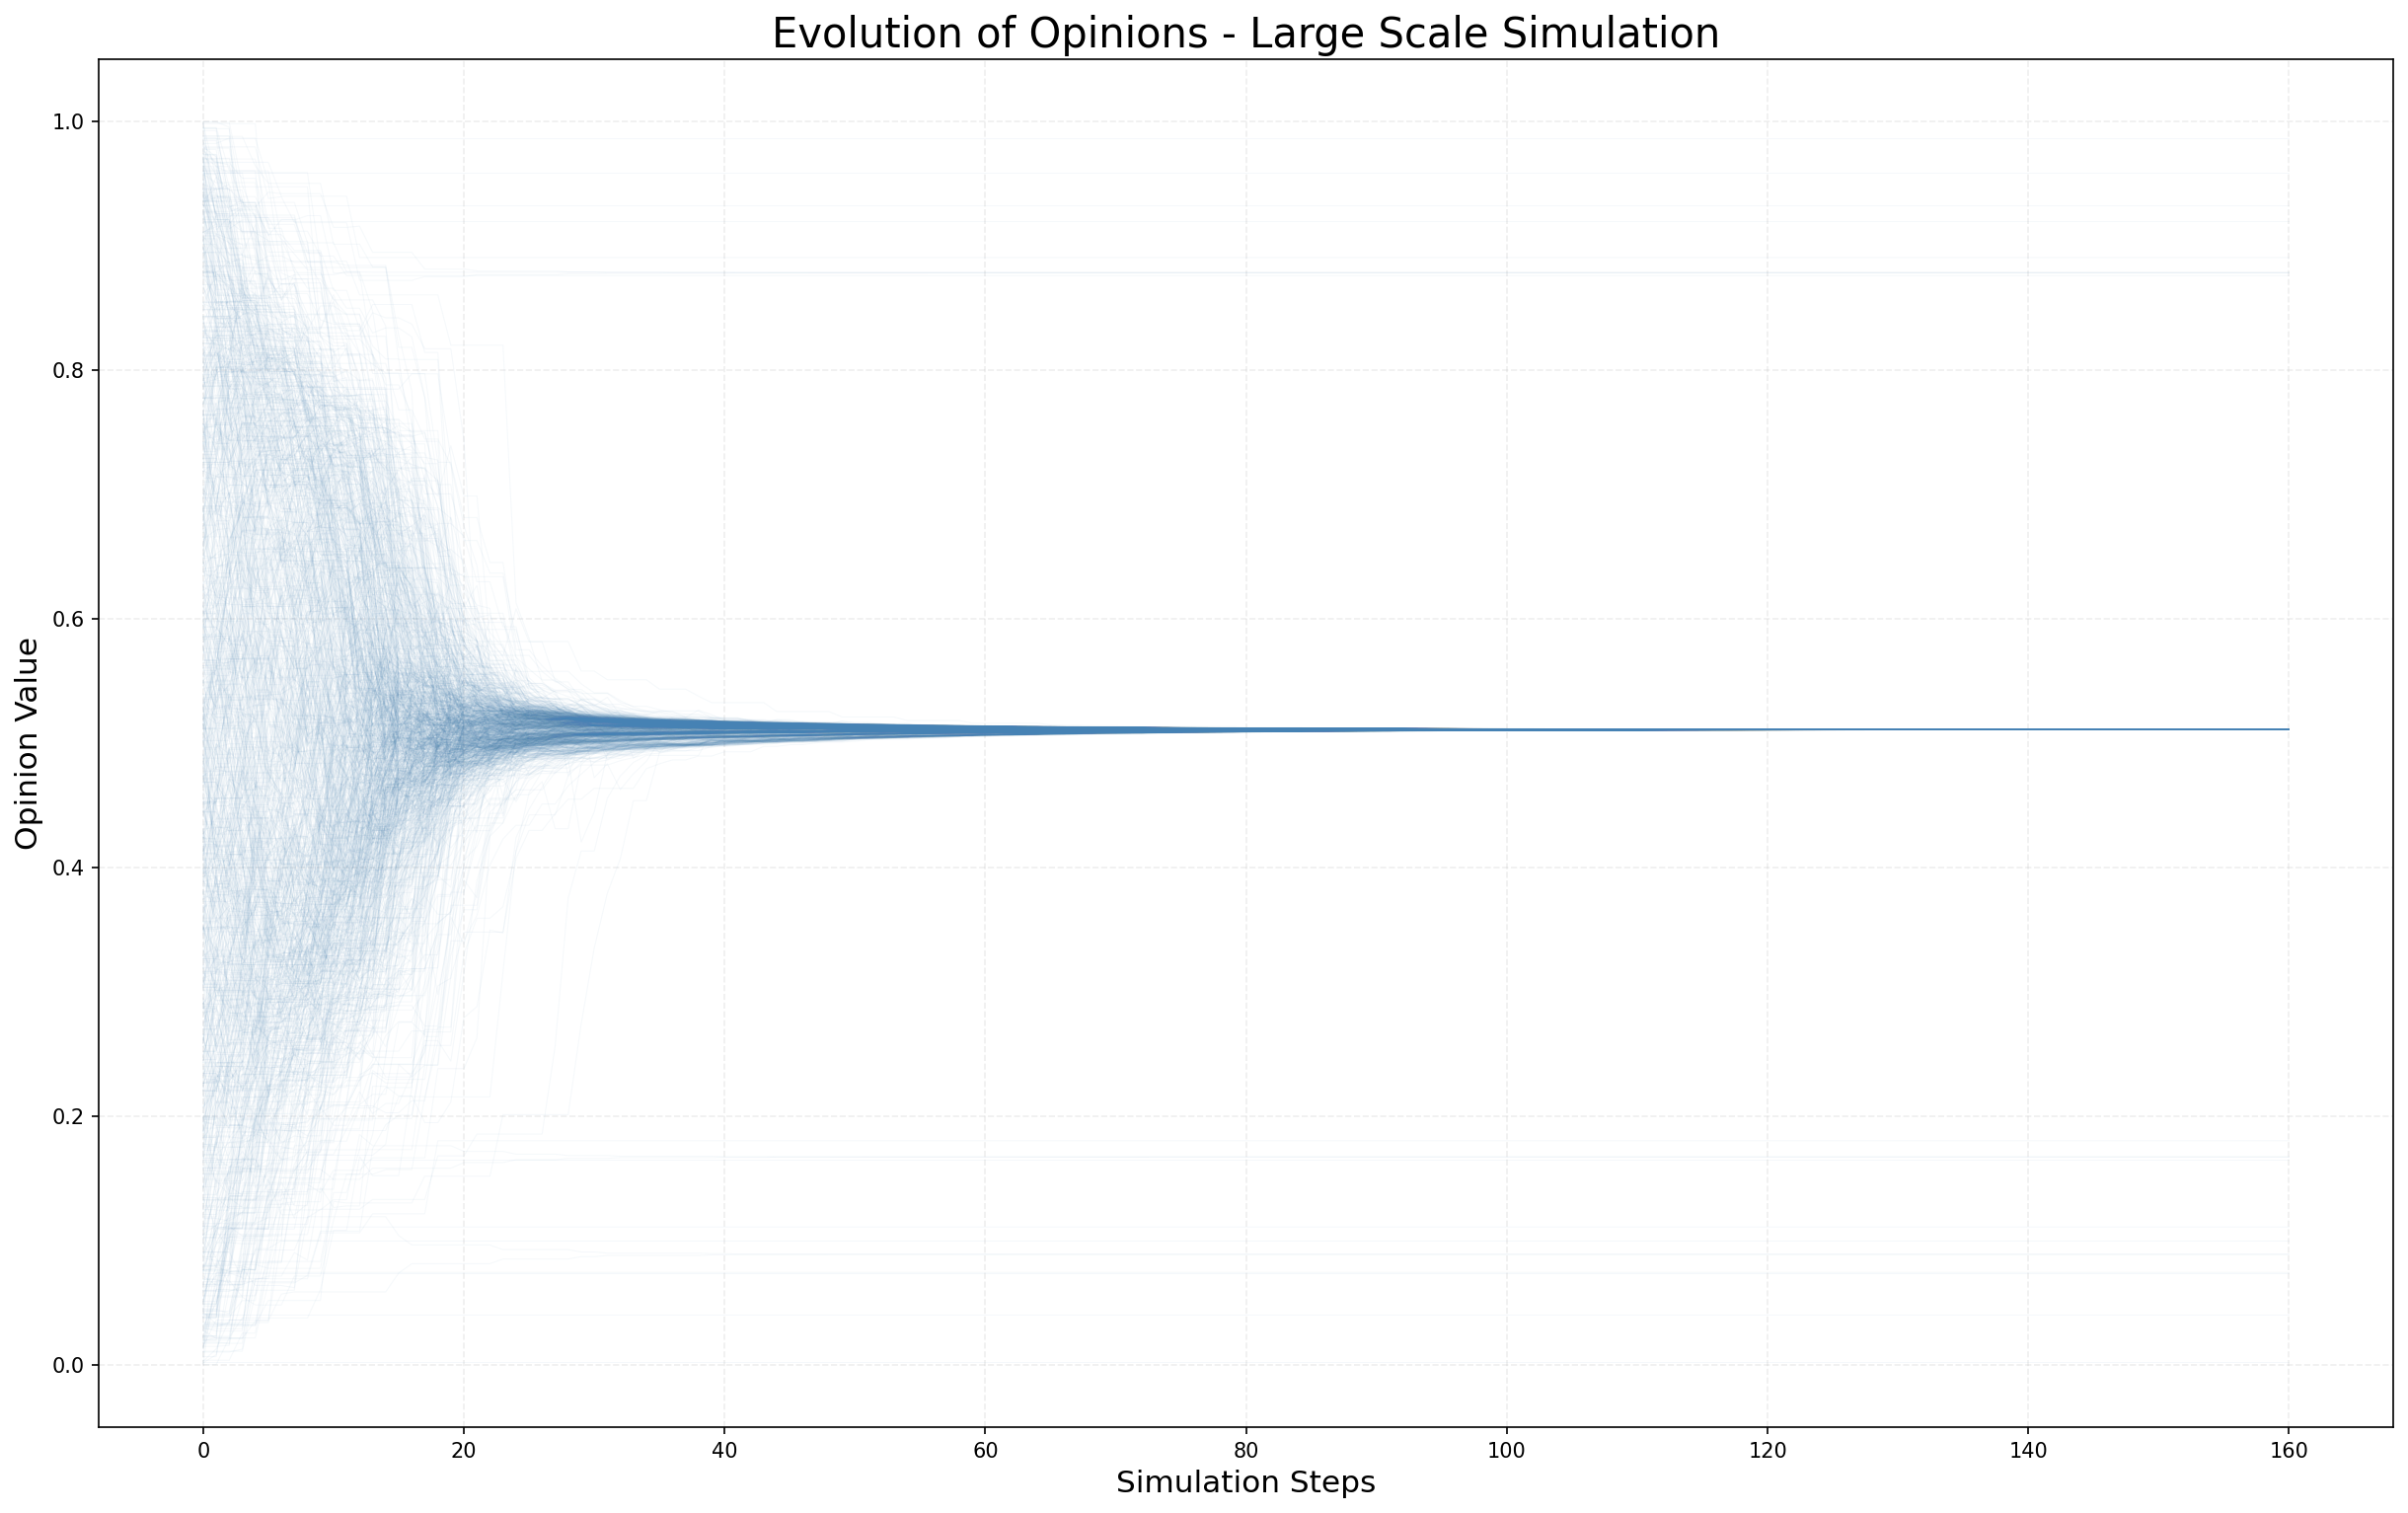
\includegraphics[width=0.33\linewidth]{results/p_0.9_threshold_0.3/opinions_history}
        \caption{Histórico de opiniones Prob. inter 0.9, confianza 0.3: Consenso}
        \label{fig:p_0.9_threshold_0.3}
    \end{figure}
    \FloatBarrier

\end{document}
